
% \documentclass[a4paper, fleqn, usenatbib, useAMS]{mnras}
\documentclass[fleqn, usenatbib]{mnras} 
\usepackage{newtxtext, newtxmath} 	% Required for MNRAS 
\usepackage[T1]{fontenc}
% \usepackage{ae, aecompl}			% Required for MNRAS
\usepackage{graphicx}
\usepackage{amsmath}
\usepackage{amssymb}
\usepackage{mathtools}
\usepackage{multicol}
\usepackage{bm}
\usepackage{pdflscape}
\usepackage{natbib}
\usepackage[section]{placeins}
\usepackage{lipsum}
\usepackage{etoolbox} 
\usepackage{tabularx} 
\usepackage{xcolor} 
\usepackage[toc, page]{appendix} 
% \hypersetup{draft} 
% \linespread{1.8} 
\hypersetup{ 
	colorlinks		= true, 
	urlcolor 		= blue, 
	linkcolor 		= blue, 
	citecolor 		= blue 
} 

\newcommand{\ddfrac}[2]{\frac{\displaystyle #1}{\displaystyle #2}} 
\newcommand{\refp}[1]{(\ref{#1})} 
\newcommand{\msun}{\ensuremath{\text{M}_\odot}} 
\newcommand{\persqkpc}{\ensuremath{\text{kpc}^{-2}}} 
\providecommand{\noopsort}[1]{} 
\graphicspath{ {../plots/} } 

\interfootnotelinepenalty = 10000 
\defcitealias{Kroupa2001}{Kroupa} 
\defcitealias{Salpeter1955}{Salpeter} 

\title[Stellar Migration and Chemical Enrichment]{Stellar Migration and 
Chemical Enrichment in the Milky Way Disk: Predictions of a Hybrid Model} 

\author[J.W. Johnson et al.]{
	James W. Johnson,$^{1}$\thanks{Contanct e-mail: \href{mailto:
	johnson.7419@osu.edu}{johnson.7419@osu.edu}} 
	David H. Weinberg,$^{1, 2}$ 
	Fiorenzo Vincenzo,$^{2}$ 
	Jonathan C. Bird,$^{3}$ 
	\newauthor 
	Sarah R. Loebman,$^{4}$ 
	Alyson Brooks,$^{5}$ 
	Thomas R. Quinn,$^{6}$ 
	Charlotte R. Christensen,$^{7}$ 
	\newauthor 
	et al.?
	\\
	$^{1}$ Department of Astronomy, The Ohio State University, 
	140 W. 18th Ave., Columbus, OH, 43210, USA 
	\\ 
	$^{2}$ Center for Cosmology and Astroparticle Physics (CCAPP), 
	The Ohio State University, 191 W. Woodruff Ave, Columbus, OH, 43210, USA 
	\\ 
	$^{3}$ Department of Physics \& Astronomy, Vanderbilt University, 
	2301 Vanderbilt Place, Nashville, TN, 37235, USA 
	\\ 
	$^{4}$ Department of Physics, University of California Merced, 
	5200 North Lake Rd., Merced, CA, 95343, USA 
	\\ 
	$^{5}$ Department of Physics \& Astronomy, Rutgers University, 136 
	Frelinghuysen Rd, Piscataway, NJ, 08854, USA 
	\\ 
	$^{6}$ Department of Astronomy, University of Washinton, Box 351580, 
	Seattle, WA, 98195, USA 
	\\ 
	$^{7}$ Department of Physics, Grinnell College, 1116 8th Ave., Grinnell, 
	IA, 50112, USA 
} 

\date{Accepted XXX; Received YYY; in original form ZZZ} 
\pubyear{2020} 

\begin{document} 
\label{firstpage} 
\pagerange{\pageref{firstpage}--\pageref{lastpage}} 
\maketitle 

\begin{abstract} 
We investigate the impact of stellar migration on galactic chemical evolution 
models, considering a handful of assumptions for the star formation history 
and time-dependence of radial migration based on a zoom-in, hydrodynamical 
simulation of galaxy evolution. We find that models for the 
time-dependence of radial migration impact the type Ia supernova rate as a 
function of both time and radius, inducing significant variability. We 
demonstrate that this is a means with which young, $\alpha$-enhanced stars can 
arise naturally out of inside-out galaxy growth with stellar migration. We find 
that the observed age-[$\alpha$/Fe] relation is well-fit by an inside-out star 
formation history, while the age-[O/H] and age-[Fe/H] relations are well-fit by 
a late starburst model; no one model investigated here fits both 
simultaneously. Our model successfully reproduces the broad nature of the 
[$\alpha$/Fe] distribution at fixed [Fe/H] in a given Galactic region; however, 
an overprediction of the frequency of intermediate [$\alpha$/Fe] stars prevents 
it from explaining the observed results in detail. This suggests 
that inside-out galaxy growth combined with radial migration, even with a late 
starburst, is not conducive to forming the infamous bimodality as it is 
observed. We postulate that more dramatic evolutionary scenarios (e.g. a 
two-infall model) may be necessary to describe the observed results. In 
conducting this analysis, we developed and made use of newly released features 
in the \texttt{Versatile Integrator for Chemical Evolution} (\texttt{VICE}) 
which are built to handle these simulations under a wide variety of 
assumptions. \texttt{VICE} is publicly available 
at~\url{https://pypi.org/project/vice}. 
\end{abstract} 

\begin{keywords} 
methods: numerical -- galaxies: abundances, evolution, star formation, stellar 
content 
\end{keywords} 

\section{Introduction} 
\label{sec:intro} 
\begin{itemize} 
	\item Known for some time that stars undergo radial migration 
	\citep[e.g.][]{Wielen1996}; this is an effect which could considerably 
	impact chemical evolution in galaxies by mixing stars that formed in 
	different galactic regions with significantly different enrichment 
	histories. 

	\item To date there are only a handful of models which attempt to include 
	this information, all focused on the Milky Way~\citep[e.g.][]{Matteucci1989, 
	Schoenrich2009, Minchev2013, Sharma2020}. Each of these 
	studies treated the Milky Way as a series of concentric annuli, each 
	described by a conventional one-zone model with parameters that change from 
	annulus to annulus. In the resultant ``multi-zone'' model, stars and gas 
	migrate between zones under some prescription to account for mixing 
	processes. In this paper, we adopt an approach similar to that used by 
	\citet{Minchev2013}, in which the mixing processes are informed by star 
	particles from a hydrodynamical simulation ran from cosmological initial 
	conditions. With parameters tuned to reproduce observed results, such as 
	abundance and surface density gradients, we can then assess the model 
	predictions to address the following question: when combining simple, 
	conventional assumptions about the star formation and dynamical histories 
	of the Milky Way, what observed results can be replicated? 
	
	\item The observables that we focus on are: 
	\begin{itemize} 
		\item Metallicity distributions and abundance gradients 

		\item The [$\alpha$/Fe] bimodality 

		\item The age-metallicty relation (AMR) 

		\item The young, $\alpha$-rich population
	\end{itemize} 

	\item Metallicity Distributions and the Abundance Gradient 
	\begin{itemize} 
		\item Known for some time that the inner regions of Milky Way-like 
		spirals are more metal-rich than their outskirts (SDSS references: 
		\citealp{Nordstroem2004a, Daflon2009, Frinchaboy2013, Hayden2014}). 
		There are variations depending on what type of stars are considered 
		and what metallicity tracers are used. This qualitative result is 
		also seen in the gas-phase~\citep[see, e.g., the results from the 
		CHAOS project using HII regions;][]{Berg2015, Berg2020}. 

		\item We know from APOGEE data that the observed MDF has a metal-poor 
		mode and is skew-positive in the outer galaxy (and conversely, 
		metal-rich and skew-negative in the inner galaxy; 
		\citealp{Hayden2015}). The variation with Galactocentric radius is 
		usually attributed to radial migration of metal-poor (metal-rich) 
		stars from larger (smaller) radii, the same argument that 
		\citep{Sellwood2002} used to interpret the results of 
		\citet{Edvardsson1993} on the observed AMR in the solar neighborhood. 

		\item Abundance gradients have been the focus of many studies and 
		are quantified rather extensively, but 
		their origin is somewhat up for debate. Applying the analytic models 
		of~\citet{Weinberg2017}, one could argue that the gradient arises out 
		of variations in the local gas-phase equilibrium abundance as a 
		function of Galactocentric radius. This could be due to variations in 
		the efficiency of outfowing winds removing metals from the star 
		forming reservoir due to a deeper gravitational potential in the inner 
		regions of Milky Way-like spirals.~\citet{Nidever2014} used this 
		methodology to successfully reproduce the APOGEE abundance data. 
		However, recent chemical evolution models have successfully replicated 
		the gradient with no outflowing winds at all 
		\citep[e.g.][]{Minchev2013, Spitoni2019}. This is based on arguments 
		from~\citet{Melioli2008, Melioli2009} and~\citet{Spitoni2008, 
		Spitoni2009}, who studied Galactic fountains and found that ejected 
		metals tend to reaccrete to a Galactocentric radius similar to where 
		they originated. With this result, some authors argue that such 
		outflows do not significantly alter the chemical evolution of a 
		Galactic disc. A notable difference between these two models is that 
		the latter requires significantly lower nucleosynthetic yields to 
		predict physically realistic abundances. 
	\end{itemize} 

	\item The [$\alpha$/Fe] bimodality 
	\begin{itemize} 
		\item Milky Way stars segregate themselves into the low- and 
		high-$\alpha$ sequences, a bimodality found in, e.g., 
		Gaia ESO~\citep{Recio-Blanco2014, Rojas-Arriagada2017}, and 
		APOGEE~\citep{Nidever2014, Hayden2015, Weinberg2019}. 

		\item Presence is well established, though origin a topic of intense 
		debate. 

		\item Notion that it could arise out of radial migration traces back 
		to~\citet{Schoenrich2009}. 

		\item \citet{Weinberg2017} models suggest increase in strength of the 
		mass-loading factor $\eta$ at late times would lower the equilibrium 
		abundance, forming stars along the low-$\alpha$ sequence. This plus 
		radial migration is yet unexplored. 

		\item \citet{Spitoni2019, Spitoni2020} demonstrate that two-infall 
		models can reproduce solar annulus data with good agreement. Recently, 
		\citet{Spitoni2021} argued that this extends to other regions of the 
		Galactic disc by reproducing APOGEE DR16 abundances by means of a 
		chemical evolution model with three annuli centered on 4, 8, and 12 
		kpc. Although they're able to reproduce the data for different regions 
		of the Galaxy, their model does not include a treatment for the 
		migration of stars beyond their birth radius; though with 4-kpc annuli, 
		it's not likely there would be much impact given the coarse nature of 
		the binning. 

		\item \citet{Grand2018} find with Auriga~\citep{Grand2017} that early, 
		accretion induced starburst populates the high-$\alpha$ sequence, 
		followed by low-level, sustained star formation on low-$\alpha$ 
		sequence, and a rapid transition between the two ensures chemical space 
		relatively unpopulated. This would imply short $\tau_\star$ (see 
		justification in~\citealp{Weinberg2017}). Ongoing, low-metallicity 
		gas accretion can also populate low-$\alpha$ sequence. 
		\citet{Buck2020b} find results qualitatively similar to second 
		scenario in NIHAO simulation suite~\citep{Wang2015, Buck2020a}. 
		Hydrodynamical simulations take into account radial migration by 
		construction. 

		\item \citet{Clarke2019} show that star formation proceeded in clumps 
		in an SPH simulation of an NFW halo using GASOLINE~\citep{NFW1997, 
		Wadsley2017}. The clumps self-enrich, forming stars on the 
		high-$\alpha$ sequence, while more spatially extended, smooth star 
		formation populated the low-$\alpha$ sequence. 

		\item No shortage of models that reproduce the dichotomy, yet only 
		those done with hydrodynamical simulations and a handful of others 
		have taken into account radial migration. 
	\end{itemize} 

	\item The Age-Metallicity Relation (AMR) 
	\begin{itemize} 
		\item Age-metallicity relation in the solar neighbourhood exhibits 
		considerable intrinsic scatter~\citep{Edvardsson1993}, usually 
		attributed to radial migration of metal-rich (metal-poor) stars formed 
		at smaller (larger) Galactocentric radii~\citep{Sellwood2002, 
		Haywood2008, Roskar2008b, Schoenrich2009}. 

		\item \citet{Feuillet2018} reveal that super-solar metallicity stars 
		are statistically older than solar metallicity stars (their Fig. 3). 
		Contrasts with simple one-zone models where enrichment proceeds 
		alongside star formation yielding a monotonic 
		AMR~\citep[e.g.][]{Andrews2017, Weinberg2017}. One-zone models of 
		starbursts can produce non-monotonic AMR due to the effect of 
		dilution~\citep{Johnson2020}, but they by construction do not predict 
		multiple abundances at fixed age. Argued using 
		the~\citet{Weinberg2017} 
		analytic models that this is a consequence of radial migration - for a 
		smooth star formation history (SFH), the youngest stars at any given 
		radius will have composition reflective of the local equilibrium 
		abundance, and only older stars will have had adequate time to 
		migrate to a similar Galactocentric radius. 
	\end{itemize}

	\item The Young Alpha-Rich Population 
	\begin{itemize} 
		\item Population of young ($\sim$few Gyr), [$\alpha$/Fe]~$\sim$ 
		0.1-0.2 stars in the solar neighbourhood. 

		\item Found using stellar ages estimated from carbon-to-nitrogen 
		ratios~\citep{Martig2016}, isochrone matching~\citep{Feuillet2018, 
		Feuillet2019}, and with the asteroseismic ages in the original APOKASC 
		catalog~\citep{Chiappini2015, SilvaAguirre2018, Pinsonneault2014}. 
		\citet{SilvaAguirre2018} demonstrated that these stars have 
		kinematics similar to the rest of the high-$\alpha$ population, and 
		argued based on this that they may be the consequence of stellar 
		mergers or mass transfer events, making truly old stars simply appear 
		younger. 

		\item \citet{Mor2019} infer a factor of~$\sim$2 enhancement in the 
		SFH of the Milky Way~$\sim$2 Gyr ago by comparing population synthesis 
		models to observed stellar luminosity functions and color-magnitude 
		diagrams from Gaia data~\citep{GaiaDR2}.~\citet{Isern2019} reach 
		similar conclusions by modeling the white dwarf luminosity function in 
		the solar neighbourhood with Gaia parallaxes. Motivated by these 
		results, \citet{Johnson2020} demonstrate using one-zone chemical 
		evolution models that a recent starburst can produce young, 
		$\alpha$-enhanced stars. Caveat: burst would have had to be 
		sufficiently localized such that the young,~$\alpha$-rich stars remain 
		outliers from an otherwise monotonically descreasing age-[$\alpha$/Fe] 
		relation. 
		\begin{itemize} 
			\item The impact of such evolutionary histories combined with a 
			model for stellar migration is, to our knowledge, yet unexplored in 
			the literature. 
		\end{itemize} 
	\end{itemize} 

	\item A viable model for the detailed enrichment history of the Milky Way 
	would explain simultaneously all of these observed results and their 
	variations in different Galactic regions, while also taking into account 
	effects like mixing and observational systematics. In this paper, we aim to 
	assess the extent to which conventional assumptions about the evolutionary 
	history of the Milky Way can account for these results, entertaining a 
	handful of models describing the star formation history and time-dependence 
	of radial migration. 
	\begin{itemize} 
		\item Motivated by the general result that Galaxies grow in radius 
		(i.e. ``inside-out'' growth;~\citealp{Bird2013}), our base-line model 
		has a star formation history whose e-folding timescales grow with 
		Galactocentric radius. Motivated by the findings of~\citet{Mor2019} 
		and~\citet{Isern2019}, we also construct models which exhibit a recent 
		enhancement in the star formation rate. For comparison, we also 
		construct a model in which the SFH is constant with time at fixed 
		radius; this is interesting primarily from a theoretical perspective, 
		removing the effects of a time-varying SFH to quantify only what is 
		predicted by ongoing star formation with radial mixing. 

		\item While we make use of a hydrodynamical simulation to include the 
		effects of radial migration, we do~\textit{not} make use of its star 
		formation history. While~\citet{Minchev2013} also made use of a 
		hydrodynamical simulation in their study, ours differs from theirs in 
		this key aspect. The~\citet{Schoenrich2009} and~\citet{Sharma2020} 
		studies, on the other hand, chose a model for radial migration that was 
		based on dynamical arguments, which introduced free parameters that 
		then required fitting to data. An advantage of our decision to make use 
		of a hydrodynamical simulation over dynamical arguments is that it's 
		unclear the extent to which fitting to observed data biases the model 
		into agreement with parts of the data that weren't part of the fit. A 
		hydrodynamical simulation, while still an approximation of reality, 
		is motivated by first principles in that it models the gravitational 
		interactions of star particles with gas and other star particles as 
		well as the diffuse dark matter halo. The primary disadvantage of this 
		choice is a consequence of the lack of free parameters - the model is 
		rigid, and we cannot explore slight variations. However, in principle 
		one could compare the predictions made by our chemical evolution models 
		but with different hydrodynamical simulations. 
	\end{itemize} 

\end{itemize} 

\section{Methods} 
\label{sec:methods} 

\begin{itemize} 
	\item To fulfill the goals of this paper, we develop and make use of 
	newly released features within the~\texttt{Versatile Integrator for 
	Chemical Evolution} (\texttt{VICE}), which are designed to handle these 
	kinds of simulation with a wide range of flexibility. We reserve 
	description of~\texttt{VICE}'s algorithm and our simulation parameters 
	for~\S~\ref{sec:methods:migration}, first describing our sample of star 
	particles from the hydrodynamical simulation. 

	\item We emphasize that the star particles from the hydrodynamical 
	simulation are used~\textit{only} in the mixing component of our models. 
	We make use of neither its star formation nor chemical enrichment 
	histories; rather, these are exactly what we explore variations of in this 
	paper. There is no N-body integration involved in our models. 
\end{itemize} 

\subsection{The Hydrodynamical Simulation} 
\label{sec:methods:h277} 

% fig 1 
\begin{figure*} 
\centering 
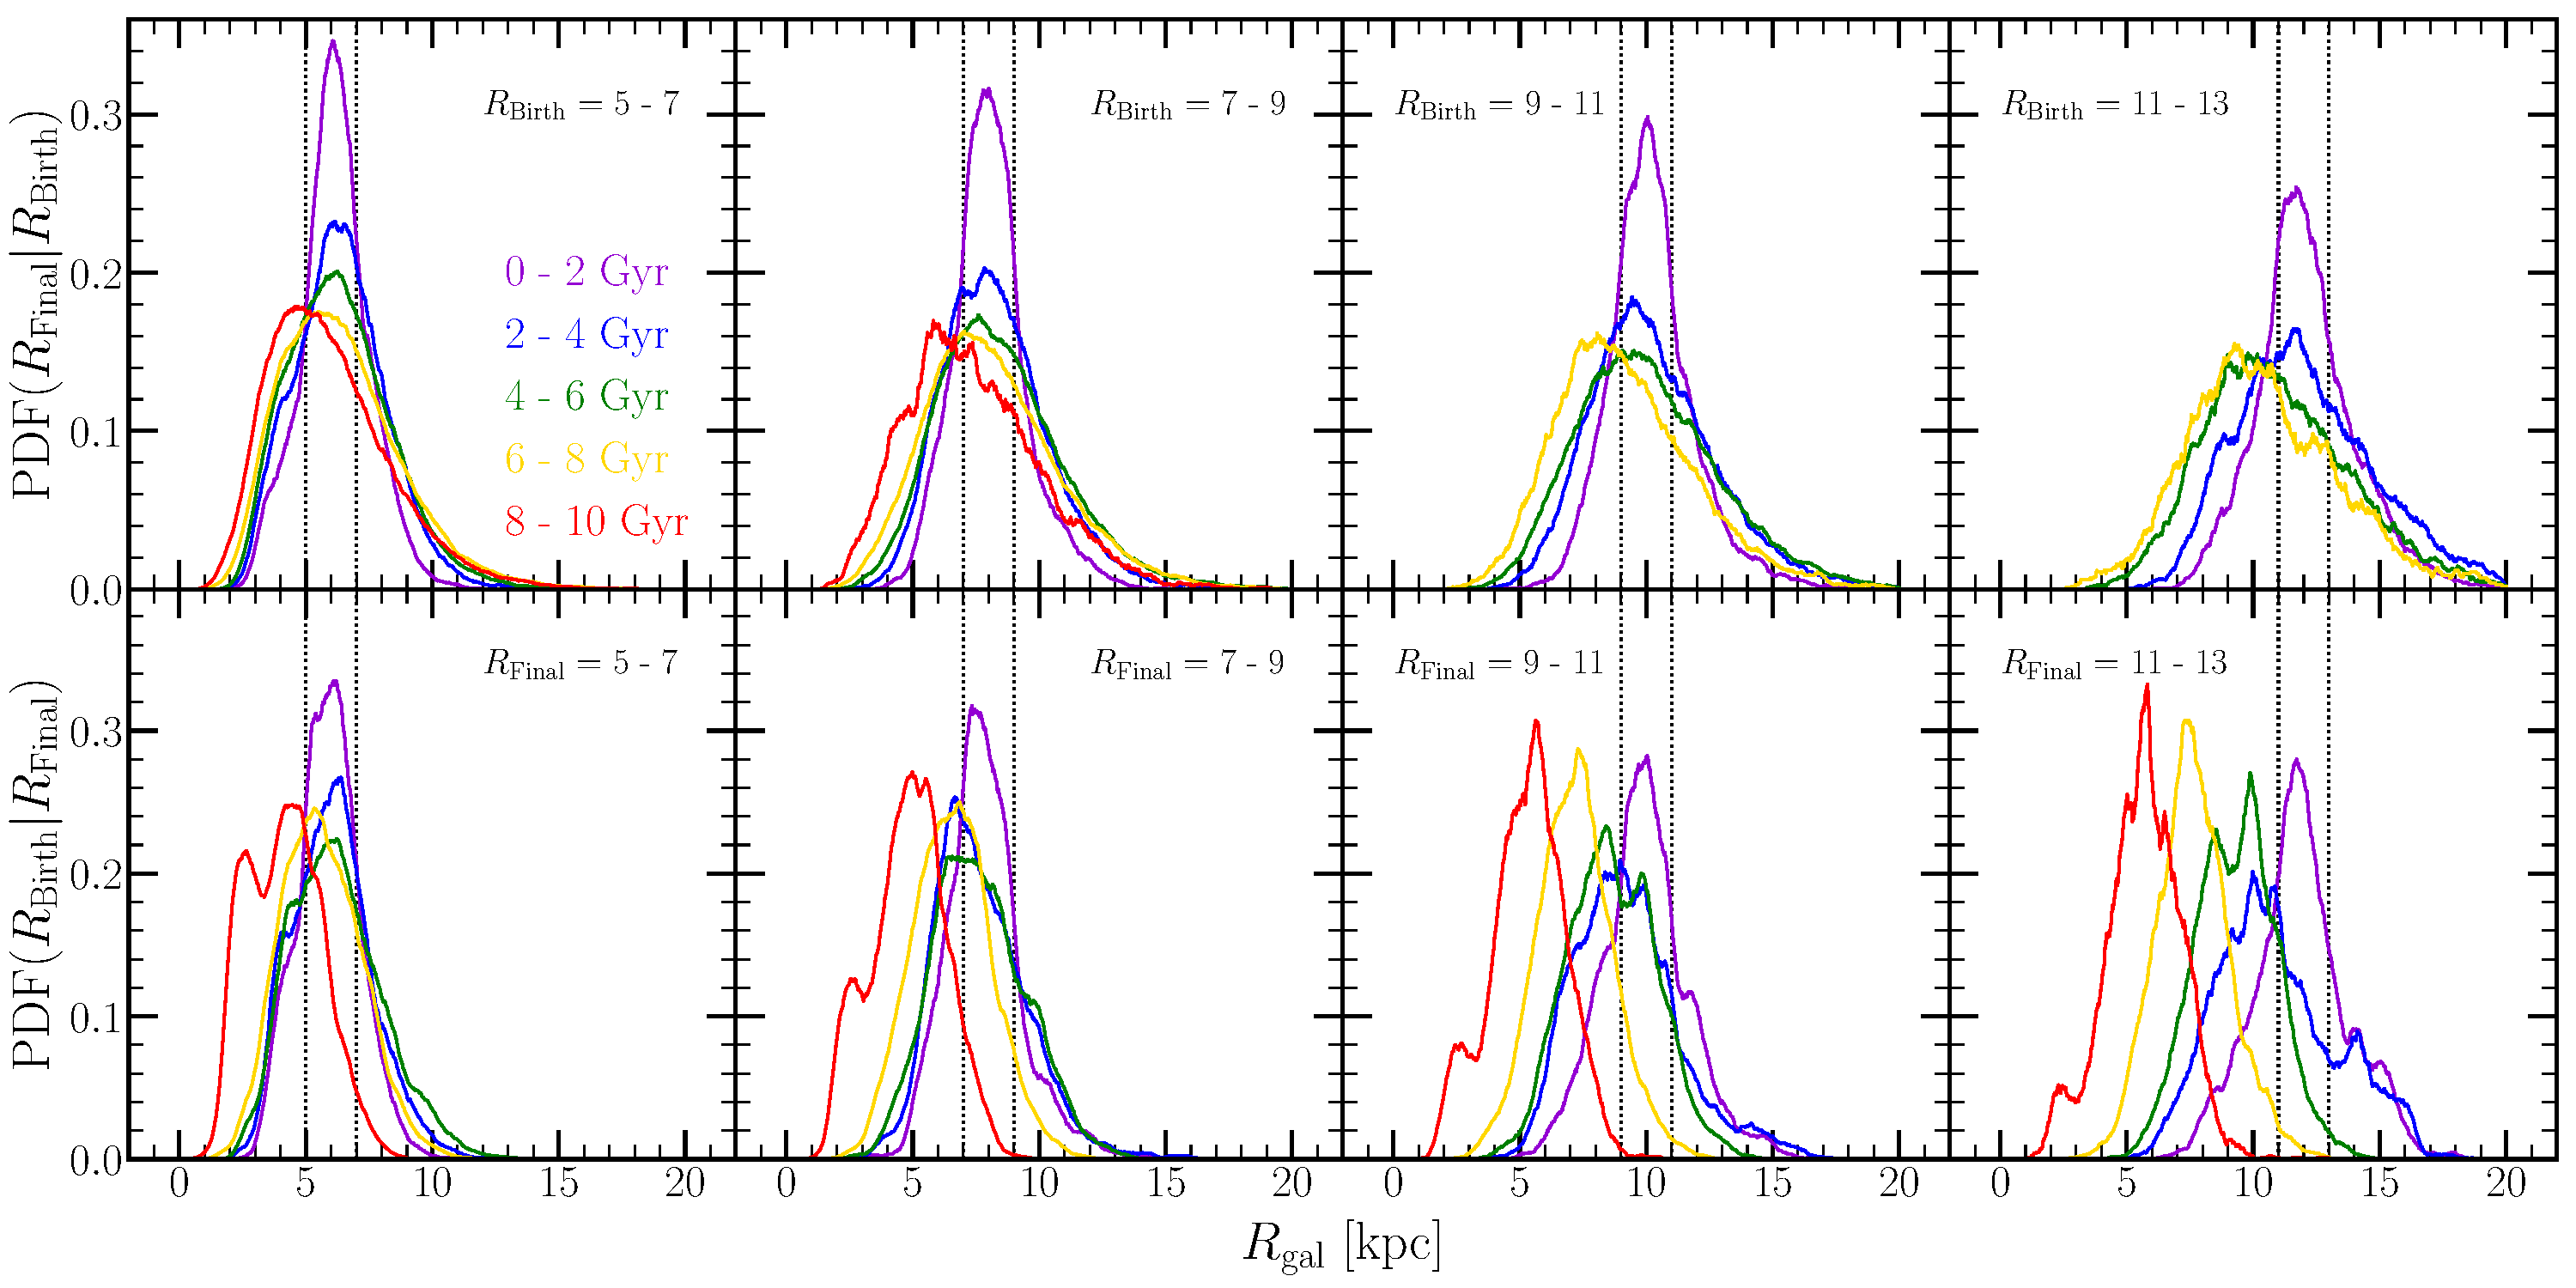
\includegraphics[scale = 0.32]{decomposition.pdf} 
\caption{Radial distributions of our candidate analog star particles 
from~\texttt{h277}. In the top row, we show distributions of~\textit{final} 
radius in bins of birth radius and age. In the bottom row, we show 
distributions of~\textit{birth} radius in bins of final radius and age. Each 
bin in Galactocentric radius is shown in its own panel, denoted in text at the 
top of each panel and by vertical black dashed lines. We color-code the 
distributions according to the age of the star particles, denoted by the 
legend in the upper left panel. We smooth all distributions with a box-car 
width of 0.5 kpc to improve clarity. We omit the distributions for 8 - 10 Gyr 
old stars born in the 9 - 11 and 11 - 13 kpc bins due to an insufficient 
number of star particles with which to calculate the distribution. }
\label{fig:h277_decomposition} 
\end{figure*} 

\begin{itemize} 
	\item In this paper we make use of star particles from the~\texttt{h277} 
	simulation~\citep{Christensen2012, Zolotov2012, Loebman2012, Loebman2014, 
	Brooks2014}. A synopsis of the detailed simulation parameters and 
	cosmological model can be found in~\S~2 of~\citet{Bird2020}. We do not 
	go into detail on that here, instead focusing on how we vet the sample of 
	star particles for use in our chemical evolution models. 

	\item Of particular importance to have accurately measured formation radii 
	for each star particle that we use in our analysis.~\texttt{h277} did not 
	record the exact birth radius of each star particle; however, each star 
	particle does have an accurate age at each snapshot. If a star particle 
	is sufficiently young in the first snapshot it appears in, then its 
	radius in that snapshot is a reasonable approximation for its birth 
	radius, since its orbit is unlikely to have changed significantly in a 
	short enough time interval. Therefore, we restrict our sample to those 
	with an age at first snapshot of~$\leq$ 150 Myr, and adopt their 
	Galactocentric radius at first snapshot as the birth radius. Also 
	conducted the analysis with age at first snapshot of~$\leq$50 Myr, and 
	found similar results, suggesting this choice does not impact our 
	conclusions. In practice, we find that 150 Myr also provides us with an 
	adequately large number of star particles to sample from. 

	\item Of the star particles with ages at first snapshot of~$\leq$~150 Myr, 
	the oldest star is 12.26 Gyr old at the present day. Since~\texttt{h277} 
	ran for 13.7 Gyr, we therefore subtract 1.5 Gyr from the formation times of 
	all star particles, and run our disc models for 12.2 Gyr. This value of 
	$T$ = 1.5 Gyr is likely tied to the onset of star formation in the 
	\texttt{h277} disc, which would have occurred some time following the 
	cosmological initial conditions at a lookback time of 13.7 Gyr. As a result, 
	our disc models trace the chemical evolution of the Milky Way out to a 
	lookback time of 12.2 Gyr, or a redshift of~$z \approx$ 3. 

	\item We further restrict the sample of star particles to only those with 
	both formation and final radii of~$R_\text{gal} \leq$~20 kpc, and to have 
	formed within~$\left|z\right|\leq$~3 kpc of the disc midplane. These 
	criteria ensure that we're only using star particles which formed in-situ. 
	While it's possible that some star particles formed in a dwarf galaxy as it 
	was infalling which would satisfy these criteria, these star particles 
	are small in number, and are only relevant at large $R_\text{gal}$ and high 
	ages, a region of parameter space where few stars form anyway. 

	\item Based on a kinematic decomposition performed on the present-day 
	phase space distribution of the~\texttt{h277} star particles, we include 
	all stars with bulge, pseudobulge, and disc-like kinematics, excluding the 
	halo stars. While we're not modeling the evolution of the bulge here, these 
	star particles are overwhelmingly located at~$R_\text{gal} \leq$~3 kpc at 
	the present day anyway, while we're interested in~$R_\text{gal} \geq$~3 kpc 
	in this paper since we're modeling the disc. This yields a sample of 
	3,000,556 star particles from~\texttt{h277}. 

	\item \texttt{h277} had a transient bar during its evolution, but does 
	not have a bar at $z$ = 0. The~\citet{Minchev2013} model, and by extension 
	the~\citet{Minchev2014} and~\citet{Minchev2017} models as well, selected a 
	hydrodynamical simulation specifically so that it would have a bar at 
	$z$ = 0. This could mean that the dynamical history of our models Galaxies 
	do not reflect that of the~\citet{Minchev2013} model, and perhaps the 
	Milky Way itself. A detailed investigation on the impact of bar evolution 
	on stellar migration and thus chemical evolution is outside the scope of 
	this paper, though can be conducted in principle by simply swapping the 
	\texttt{h277} data within~\texttt{VICE} for another simulation, then 
	rerunning our numerical models and comparing the results. 

	\item Distributions of final radii in bins of birth radii and age are 
	shown in the top row of Fig.~\ref{fig:h277_decomposition}. Conversely, the 
	bottom row shows distributions of birth radii in bins of final radii and 
	age. 
	\begin{itemize} 
		\item Focusing on the top row of panels in 
		Fig.~\ref{fig:h277_decomposition}, we note that for stars born at any 
		radius and time, the distribution of final radii is still peaked near 
		the birth radius. With increasing age, it appears the mode final radius 
		may move slightly inward. The tails of the distributions to large radii 
		are relatively age-independent - some differences between the 0 - 2 and 
		8 - 10 Gyr age bins, but not much. However, the tails of the 
		distributions to small radii are not age-independent, and move toward 
		smaller $R_\text{gal}$ with increasing age. This suggests that radial 
		migration inward and outward occur on different timescales, in 
		particular that inward migration is slower than 
		outward migration. By extension this may suggest that inward and 
		outward migration are tied to different physical 
		processes.~\citet{Roskar2008a} demonstrate using a cosmological 
		simulation that resonant scattering at corotation causes stars to 
		move outward and gas to move inward. It's possible that radial 
		migration inward has different origins. 

		\item Focusing on the bottom row of panels in 
		Fig.~\ref{fig:h277_decomposition}, we note that the oldest stars at any 
		Galactocentric radius at the present day were overwhelmingly born at 
		smaller radii. The youngest stars, however, were overwhelmingly born at 
		comparable radii, and the stars of intermediate ages simply span the 
		range in radii between the two. With increasing radius, the 
		differences in the mode of the birth radius distribution between age 
		bins gets larger. 

		\item The differences in distributions shown in the top and bottom 
		panels boils down to stellar surface density being a strong function 
		of Galactocentric radius. Take for example the age = 8 - 10 Gyr bin in 
		both $R_\text{Birth}$ = 5 - 7 kpc and $R_\text{Final}$ = 11 - 13 kpc 
		bins (i.e. the red curves in the top-left and bottom-right panels). 
		For these old stars born at 5 - 7 kpc, 11 - 13 kpc is far down the tail 
		of the $R_\text{Final}$ distribution, and yet 5 - 7 kpc is the mode 
		$R_\text{Birth}$ of all old stars presently at these radii. This 
		implies that even though the majority of 8 - 10 Gyr old stars with 
		$R_\text{Final}$ = 11 - 13 kpc were born at 5 - 7 kpc, they make up 
		only a small fraction of the stars with similar birth radii. This is 
		only possible if the stellar surface density gradient is sufficiently 
		steep, which it is known to be~\citep[e.g.][]{Bland-Hawthorn2016}. 
		\begin{itemize} 
			\item Fig.~\ref{fig:h277_decomposition} also demonstrates that the 
			numbers of stars that migrated inward and outward are comparable 
			in~\texttt{h277}. Taking a~$\left|\Delta R_\text{gal}\right| \geq$ 
			500 pc between birth and final radii as the criterion for migrating 
			inward or outward, indeed we find that in our sample, 27\% 
			migrated inward, 29\% migrated outward, and the remaining 44\% 
			stayed near their birth radius. These are global percentages. 
		\end{itemize} 

		\item In all bins of birth radius, a good first-order estimate of the 
		probability density that a star has a final radius in the same bin 
		is~$\sim$0.3. With bins in radius on this plot of 2 kpc, this suggests 
		that ~$\sim$40\% of stars migrate significantly by the time 
		they're~$\sim$2 Gyr old. If the SN Ia DTD is a 
		$t^{-1.1} \approx t^{-1}$ power-law as suggested by recent 
		observations~\citep[e.g.][]{Maoz2012, Maoz2017}, 
		then we expect similar numbers of SN Ia events to occur with delay 
		times between 1 and 10 Gyr as we do between 100 Myr and 1 Gyr. With 
		such an extended DTD, and the distributions in final radius shown in 
		the bottom panel of Fig.~\ref{fig:h277_decomposition}, its possible 
		that white dwarfs migrate significant distances before producing a SN 
		Ia event. Indeed, in the ASAS-SN bright supernova catalog,~$\sim$10\% 
		of supernovae are seen at >10 kpc from their host galaxies 
		\citep{Holoien2019}. While this catalog is for~\textit{all} 
		supernovae, the majority of SN events are type Ia anyway. Based on 
		this, it's reasonable to expect that the migration 
		of nucleosynthetic yields may proceed alongside stellar migration, an 
		effect which is often neglected (e.g.~\citealp{Minchev2013}, and the 
		application of the~\citealp{Weinberg2017} analytic models in 
		\citealp{Feuillet2018}). In this paper, we relax this assumption. The 
		application of the~\texttt{h277} star particle data to our model for 
		radial migration and the time dependence thereof is discussed in the 
		next section. 

	\end{itemize} 

\end{itemize} 


\subsection{Radial Migration} 
\label{sec:methods:migration} 
\begin{itemize} 
	\item To simulate our models, we develop and make use of \texttt{VICE}'s 
	\texttt{milkyway} object, an extension of a more general object named 
	\texttt{multizone}. The \texttt{multizone} object is at its core an array 
	of \texttt{singlezone} objects, which are designed to handle 
	simulations of one-zone models and were the focus of 
	\citet{Johnson2020},~\texttt{VICE}'s initial release paper. The 
	\texttt{multizone} object then affords the user the ability to move 
	gas between zones with any given time dependence, and to assign all 
	stellar populations any given zone at any given time following their 
	birth, effectively allowing arbitrarily complex zone and migration 
	schema. The \texttt{milkyway} object is a user-friendly extension of this 
	which enforces a zone configuration in which the Galaxy is modeled as a 
	series of concentric annuli of uniform width~$\Delta R_\text{gal}$. As 
	defaults, it adopts the stellar migration model described in this section 
	and our star formation law described in~\S~\ref{sec:methods:sfe}. 

	\item Stars in~\texttt{VICE} are stand-ins for entire stellar 
	populations, and in the~\texttt{milkyway} object, are said to be in a 
	given zone/annulus if their radius is between the inner and outer 
	edges. At all times, their nucleosynthetic products and returned envelopes 
	are placed in the ISM of the annulus that they are in~\textit{at that 
	time}. 

	\item Where hydrodynamical and N-body simulations of galaxy evolution 
	often use star particles of a fixed mass,~\texttt{VICE} forms a fixed 
	number of stellar populations in a given zone at a given timestep, 
	and allows their masses to vary to account for variations in the star 
	formation rate. The mass of stars formed in a given zone is divided 
	evenly among the stellar populations that form during a given 
	timestep. 

	\item Algorithm based on initial and final radii of star particles in 
	hydrodynamical simulations, for which we've taken~\texttt{h277} as 
	discussed in the previous section. 

	\item In modeling the Milky Way as a series of concentric annuli,
	~\texttt{VICE}'s~\texttt{milkyway} object assumes stellar populations to 
	be born at the centres of each annulus. For a stellar population born at a 
	time~$T$ and Galactocentric radius~$R_\text{gal}$, it first searches for 
	star particles from~\texttt{h277} that formed at~$T \pm$ 250 Myr and 
	$R_\text{gal} \pm$ 250 pc. It then randomly selects a star particle from 
	this subsample with no bias to act as an~\textit{analog}. This stellar 
	population then assumes the change in orbital radius~$\Delta R_\text{gal}$ 
	of its analog at face value, and moves from its birth radius to the implied 
	final radius at $T$ = 12.2 Gyr with some time dependence. If no candidate 
	analogs are found,~\texttt{VICE} widens the search to~$T \pm$ 500 Myr and 
	$R_\text{gal} \pm$ 500 pc. While the maximum allowed difference in birth 
	times caps here at 500 Myr, we allow the difference in birth radii to 
	continue increasing by 250 pc until a candidate analog is found. 
	\begin{itemize} 
		\item In principle this allows stellar populations to be assigned 
		analogs with significantly different birth radii; however, this is only 
		an issue for small~$T$ and large~$R_\text{gal}$ where there are few 
		star particles from~\texttt{h277}, and where few stars form in nature 
		anyway due to the inside-out growth of Galaxies. Furthermore, due to 
		the similarity of the histograms in the top row of Fig. 
		\ref{fig:h277_decomposition}, we expect taking~$\Delta R_\text{gal}$ 
		from a star particle which formed at a similar time but different birth 
		radius in these instances to be accurate enough for our purposes. 

		\item Each annulus in our models does not contain any vertical 
		information; that is, the displacements of stars from the disc midplane 
		$\left|z\right|$ does not enter into our models at all. After running 
		a~\texttt{VICE} simulation, each stellar population is simply assumed 
		to be located at the present-day~$z_\text{final}$ of its assigned 
		analog. In effect, this retains the assumption that the gas-phase 
		abundances are verticaly and azimuthally well-mixed, and that changes 
		in the gas composition at a given time happen only in the radial 
		direction.

		\item When a star particle is assigned as an analog to a stellar 
		population in our simulations, it is~\textit{not} thrown out of the 
		sample of candidate analogs, in theory allowing a star particle to act 
		as an analog for multiple stellar populations. This is a difference 
		between the~\citet{Minchev2013} model and ours. Where we assign star 
		particles to stellar populations for which~\texttt{VICE} then 
		calculates a stellar mass and composition based on an assumed star 
		formation history, the~\citet{Minchev2013} model assigns compositions 
		to star particles. 
	\end{itemize} 

% fig 2 
\begin{figure} 
\centering 
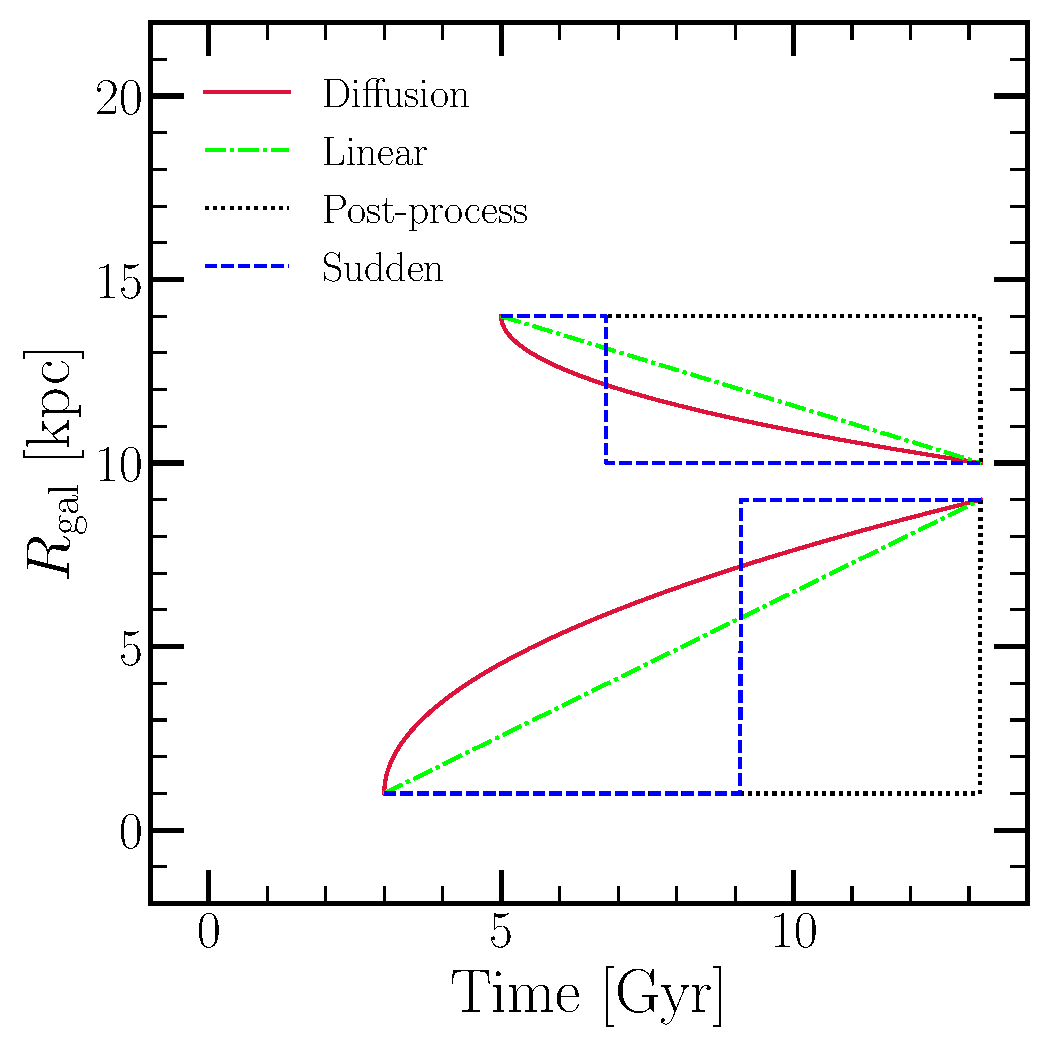
\includegraphics[scale = 0.45]{migration.pdf} 
\caption{A diagram illustrating how Galactocentric radius changes with time 
for two stellar populations under our migration schema: diffusion (crimson, 
solid), linear (lime, dot-dashed), post-process (black, dotted), and 
sudden (blue, dashed). Here the initial and final radii and birth times are 
chosen at random for illustrative purposes. With the initial and final 
Galactocentric radii of a stellar population, its birth time, and one of these 
assumptions about the time-dependence of migration, the Galactocentric radius 
at all times is known. } 
\label{fig:migration_schema} 
\end{figure} 

	\item Our migration models 
	\begin{itemize} 
		\item With our data from the~\texttt{h277} simulation 
		providing a stellar population born at some radius~$R_\text{gal}$ and 
		time~$T$ with the required~$\Delta R_\text{gal}$, we construct the 
		following four models describing the time-dependence with which a 
		stellar population moves to its final radius. 

		\item All models here neglect radial gas flows, this paper instead 
		focusing on these simple models describing how orbital radii change 
		with time. Investigation of our models with radial gas flows would be 
		an interesting extension to this paper. 

		\item \textbf{Post-processing}: Stars stay where they are born until 
		the final timestep. Based on the assumption that stellar populations 
		do not contribute to enrichment beyond their birth 
		radius~\citep[e.g.][]{Minchev2013}. Each annulus simulated as a 
		one-zone model independent of all other zones. Shown in black dotted 
		line in Fig.~\ref{fig:migration_schema}. 

		\item \textbf{Sudden}: A random number is drawn from a uniform 
		distribution between the time of birth and the present day. That time 
		is taken to be the time of instantaneous migration to the present-day 
		annulus. Emulates a scenario in which a single dynamical interaction 
		changes the orbital radius of a star. Can be thought of as a 
		time-dependent extension of the post-processing scenario. Shown in 
		blue dashed line in Fig.~\ref{fig:migration_schema}. 

		\item \textbf{Diffusion}: A case in which stars migrate in a 
		continuous, time-dependent manner. If stars move to their final 
		radii via a random walk, then the mean displacement of stars that 
		migrate similar distances would scale with~$\sqrt{\text{age}}$. This 
		is shown in the red solid line in Fig.~\ref{fig:migration_schema}. 
		This is our fiducial migration model; we present results using this 
		model except where otherwise noted. It is so named because it 
		corresponds to a scenario in which the random walk carries out the 
		diffusion of angular momentum. This is qualitatively similar to 
		\citet{Frankel2018, Frankel2020}, who also model radial orbit migration 
		with a~$\sqrt{\tau}$ dependence. 

		\item \textbf{Linear}: A simple variation of the 
		diffusion model. Has no physical motivation other than numerical 
		ease, but together with the diffusion model constitutes a test of how 
		sensitive our models are to the assumed time-dependence of stellar 
		migration. Demonstrated by green dot-dashed line in 
		Fig.~\ref{fig:migration_schema}. 
	\end{itemize} 

	\item Further details on the implementation of the~\texttt{milkyway} 
	object, the more general~\texttt{multizone} object, and other features of 
	\texttt{VICE} can found in its documentation.~\footnote{
		\url{https://vice-astro.readthedocs.io} 
	}

	\item We have a sample of 3,000,556 candidate analog star particles from 
	\texttt{h277}, only~$\sim$57\% of which are disc stars. Since we're 
	modeling the thin and thick disc populations here,~$\sim$1.71 million is a 
	much better estimate of the number of analogs that we can realistically 
	sample from. We take~$\Delta R_\text{gal}$ = 100 pc as the width of each 
	annulus from~$R_\text{gal}$ = 0 to 20 kpc and a timestep size of 
	$\Delta T$ = 10 Myr from $T$ = 0 to 12.2 Gyr (see discussion in~\S 
	\ref{sec:methods:h277} for our choice of time-interval). With the resulting 
	200 zones and 1,221 timesteps, we let~\texttt{VICE} from~$n$ = 9 stellar 
	populations per zone per timestep, resulting in 2,197,800 total stellar 
	populations with predicted masses and abundances. While this is more than 
	the number of disc particles in our sample of candidate analogs, we force 
	the star formation rate to zero beyond~$R_\text{gal}$ = 15.5 kpc; while 
	these stellar populations exist within~\texttt{VICE} and are a part of the 
	computational overhead, they have zero mass and thus do not contribute to 
	the chemical evolution. This results in 1,692,306 stellar populations 
	with~\textit{non-zero} masses and abundances predicted by~\texttt{VICE}, 
	reasonably within the limit of what we can sample. These simulations run in 
	$\sim$6 hours and take up~$\sim$235 MB of disc space per output, including 
	the extra data that we record for each stellar population's analog star 
	particle. 

	\item We emphasize that~\texttt{h277} provides our model with~\textit{only} 
	the~$\Delta R_\text{gal}$ and~$z_\text{final}$ for each individual stellar 
	population. We do not use the SFH of~\texttt{h277} or its chemical 
	enrichment history in any way, making use of only the dynamical history. 
	There is no N-body algorithm embedded within~\texttt{VICE} determining the 
	positions of stars at times between their birth and the present day. 
\end{itemize} 


\subsection{Nucleosynthetic Yields, Outflows, and Recycling}  
\label{sec:methods:yields} 
\begin{itemize} 
	\item \textit{Fractional net} yields, as required by~\texttt{VICE}. 
	Recycling is implemented separately, such that stellar envelopes are 
	returned to the ISM at the birth composition of each stellar population. 
	\texttt{VICE} takes the general approach of returning previously produced 
	material according to a stellar lifetime model and injecting newly 
	produced nucleosynthetic products as described below. Also clarify that 
	these are not~\textit{effective} yields in that outflows are also 
	implemented separately. 

	\item CCSN events are assumed to occur immediately following the formation 
	of their progenitor stars. This is an adequate approximation, because the 
	lifetimes of massive stars are short compared to the relevant timescales 
	for galaxy evolution. For the most massive stars, the lifetimes are 
	comparable to the timestep size that we take use in these simulations 
	anyway. This assumption implies a linear relationship between CCSN 
	enrichment and the star formation rate: 
	\begin{equation} 
	\dot{M}_x^\text{CC} = y_x^\text{CC}\dot{M}_\star 
	\end{equation} 
	\begin{itemize} 
		\item Physically, the CCSN yield $y_x^\text{CC}$ is the fraction of a 
		stellar population's initial mass that is converted into some element 
		$x$ and ejected to the ISM, neglecting outflows. 

		\item Take $y_\text{O}^\text{CC}$ = 0.015 and $y_\text{Fe}^\text{CC}$ 
		= 0.0012 from~\citet{Johnson2020}, who in turn adopt these values 
		from~\citet{Weinberg2017}. 
	\end{itemize} 

	\item SN Ia products injected with a $t^{-1.1}$ delay-time distribution 
	(DTD) with a minimum delay-time of $t_\text{D}$ = 150 Myr. This is the 
	default DTD in~\texttt{VICE}, adopted in~\citet{Johnson2020}, and is 
	suggested by recent observational results comparing the cosmic SN Ia rate 
	to the cosmic SFH~\citep{Maoz2012, Maoz2017}. In a 
	one-zone model at times $t > t_\text{D}$, the enrichment rate for some 
	element~$x$ can be expressed as the product of some yield $y_x^\text{Ia}$ 
	and the star formation history weighted by the DTD: 
	\begin{subequations}\begin{align} 
	\dot{M}_x^\text{Fe} &= y_x^\text{Fe}\langle\dot{M}_\star\rangle_\text{Ia} 
	\label{eq:mdot_ia} 
	\\ 
	&= y_x^\text{Fe} \ddfrac{
		\int_0^{t - t_\text{D}} \dot{M}_\star(t') R_\text{Ia}(t - t') dt' 
	}{
		\int_{t_\text{D}}^{t_\text{max}} R_\text{Ia}(t - t') dt' 
	} 
	\label{eq:mdot_ia_expanded} 
	\end{align}\end{subequations} 
	where $R_\text{Ia}$ is the DTD itself, in units of M$_\odot^{-1}$ 
	Gyr$^{-1}$. Like the CCSN yield,~$y_x^\text{Ia}$ is simply the fraction of 
	a single stellar population's mass that is converted into the element~$x$ 
	over the ensuing SN Ia duty cycle. It can also be expressed as an integral 
	over the DTD: 
	\begin{equation} 
	y_x^\text{Ia} = m_x^\text{Ia} \int_{t_\text{D}}^{t_\text{max}} 
		R_\text{Ia}(t) dt = m_x^\text{Ia} \frac{N_\text{Ia}}{M_\star} 
	\label{eq:y_x_ia} 
	\end{equation} 
	where the~$m_x^\text{Ia}$ is the mass of some element~$x$ produced in a 
	single SN Ia event on average, and the integral evaluates to the mean 
	number of Ia events~$N_\text{Ia}$ per mass of stars formed~$M_\star$. 
	\begin{itemize} 
		\item \texttt{VICE} enforces~$t_\text{max}$ = 15 Gyr always, though 
		provided one is consistent with equations~\refp{eq:y_x_ia} and 
		\refp{eq:mdot_ia_expanded}, the results are independent of 
		$t_\text{max}$ since the integrals cancel. 

		\item Extending this to multi-zone models is simple - rather than an 
		integral over the star formation history of a given annulus, the rate 
		becomes a summation over all stellar populations that are in a given 
		zone at some time: 
		\begin{equation} 
			\dot{M}_x^\text{Ia} = y_x^\text{Ia} \ddfrac{
				\sum_i M_i R_\text{Ia}(\tau_i) 
			}{
				\int_{t_\text{D}}^{t_\text{max}} R_\text{Ia}(t) dt 
			} 
		\end{equation} 
		where~$M_i$ and~$\tau_i$ are the mass and age of the~$i$'th stellar 
		population, respectively. 

		\item Initially adopt~$y_\text{O}^\text{Ia}$ = 0 and 
		$y_\text{Fe}^\text{Ia}$ = 0.0017 from~\citet{Johnson2020} and 
		\citet{Weinberg2017}. However, in practice we find that the e-folding 
		timescales of star formation in our models are sufficiently long (see 
		discussion in~\S~\ref{sec:methods:sfhs}) such that our fiducial, 
		inside-out SFH model predicts [O/Fe]~$\approx$~+0.05 for 
		young stars. We therefore multiply this value by a factor of 
		10$^{0.1}$, adopting instead~$y_\text{Fe}^\text{Ia}$ = 0.00214 so 
		that our fiducial model predicts a late-time [O/Fe] ratio in better 
		agreement with observations. This change is likely within the 
		uncertainties in nucleosynthetic yields anyway. 

		\item Our model assumes that all supernova yields of O and Fe are 
		independent of metallicity. While this appears to be empirically true 
		for CCSN yields of these elements~\citep[e.g.][]{Weinberg2019, 
		Griffith2020}, recent evidence by~\citet{Brown2019} suggests that 
		the local specific SN Ia rate shows a strong, inverse dependence on 
		galaxy stellar mass. They argue that this may imply a metallicity 
		dependent~$R_\text{Ia}$ that produces more SN Ia events at early times 
		when the metallicity is low. While we adopt a metallicity independent 
		$y_\text{Fe}^\text{Ia}$ in this paper,~\texttt{VICE} allows users to 
		specify any functional form for $y_\text{Fe}^\text{Ia}$ as a function 
		of the total abundance by mass $Z$, allowing future studies of the 
		impact of this to proceed straight-forwardly. 
	\end{itemize} 

	\item Our model assumes that all supernova yields of O and Fe are 
	independent of metallicity. While this appears to be empirically true in 
	the Milky Way~\citep{Weinberg2019, Griffith2020}, our CCSN yields are based 
	on supernova explosion models in which all >8 M$_\odot$ progenitor produces 
	a CCSN event~\citep[e.g.][]{Chieffi2004, Chieffi2013}. Recent findings 
	with regard to black hole formation and stellar explodability have 
	demonstrated that many massive stars simply do not produce a supernova 
	explosion (see theoretical discussion by, e.g.,~\citealp{Pejcha2015}; 
	\citealp{Sukhbold2016}, and observational evidence from 
	\citealp{Gerke2015, Adams2017, Basinger2020}). Such effects would 
	necessarily lower CCSN yields of all elements. While~\texttt{VICE} includes 
	functionality with which to calculate $y_x^\text{CC}$ for some element $x$ 
	using built-in tables from supernova nucleosynthesis studies, an in-depth 
	investigation of the impact of these effects is outside the scope of this 
	paper. Such an investigation which expands the capabilities of~\texttt{VICE} 
	will be presented in Griffith et al. (2021, in prep). With regard to our SN 
	Ia yields,~\citet{Brown2019} demonstrate that the local specific SN Ia rate 
	shows a strong, inverse dependence on galaxy stellar mass. They argue that 
	this may imply a metallicity dependent~$R_\text{Ia}$ that produces more SN 
	Ia events at early times when the metallicity is low. However, these 
	metallicities are only present in our models at very early times. 
	Furthermore, when outflows are taken into account, these yields are known 
	to predict observationally plausible abundances~\citep{Andrews2017, 
	Weinberg2017}. 

	\item \citet{Weinberg2017} demonstrate that, to first order, the 
	nucleosynthetic yields of a given element and the strength of outflowing 
	winds determine the late-time equilibrium abundance in the ISM. We retain 
	their characterization of outflows here, in terms of a mass-loading 
	factor~$\eta$: 
	\begin{equation} 
	\eta \equiv \frac{\dot{M}_\text{out}}{\dot{M}_\star} 
	\end{equation} 
	Here we adopt a scaling of~$\eta$ with~$R_\text{gal}$ such that the 
	late-time equilibrium abundance as a function of radius describes a 
	metallicity gradient in agreement with observations; a similar methodology 
	was employed by~\citet{Nidever2014}. 

	\item The procedure outlined in this section makes two assumptions: 1) 
	that the equilibrium abundance at a given radius corresponds to the mode 
	of the observed MDF, and 2) that radial migration does not significantly 
	impact the overall form of the gradient. We demonstrate that this holds in 
	our simulations in~\S~\ref{sec:comp_obs:metallicity_gradient}. 

	\item For $\alpha$ elements,~\citet{Weinberg2017} defines the equilibrium 
	abundance under a constant SFH as: 
	\begin{equation} 
	Z_{\alpha,\text{eq}} = \frac{
		y_\alpha^\text{CC}
	}{
		1 + \eta(R_\text{gal}) - r
	} 
	\end{equation} 
	where $r$ is the recycling parameter ($\approx$ 0.4 for the sake of this 
	scaling with a~\citetalias{Kroupa2001} IMF; see discussion in their~\S~2.2). 
	Solving for $\eta(R_\text{gal})$ yields: 
	\begin{equation} 
	\eta(R_\text{gal}) = \frac{
		y_\alpha^\text{CC}
	}{
		Z_{\alpha,\text{eq}}
	} + r - 1 
	= \frac{y_\alpha^\text{CC}}{Z_{\alpha,\odot}}10^{-\text{mode([$\alpha$/H])}
	(R_\text{gal})} + r - 1 
	\end{equation} 

	\item A fundamental observable, the observed metallicity gradient in the 
	Milky Way has been the focus of a considerable number of studies to date. 
	\begin{itemize} 
		\item \citet{Nordstroem2004a} find a gradient of -0.099 kpc$^{-1}$ in 
		[Fe/H] in main sequence stars from GCS~\citep{Nordstroem2004b, 
		Holmberg2007}. 

		\item \citet{Daflon2009} find a gradient of -0.04 kpc$^{-1}$ in 
		[S/H] in OB stars 

		\item \citet{Frinchaboy2013} find a gradient of -0.09 kpc$^{-1}$ in 
		[M/H] in open clusters. 

		\item \citet{Hayden2014} also find -0.09 kpc$^{-1}$ in [M/H] for 
		$R_\text{gal}\gtrsim$ 6 kpc for low-$\alpha$ stars. For 
		$R_\text{gal}\lesssim$ 6 kpc, they find a relatively flat gradient. 

		\item \citet{Weinberg2019} finds -0.06 kpc$^{-1}$ in mode([Mg/H]) for 
		upper red giant branch disc stars (see their Fig. 23). 
	\end{itemize} 

	\item We assume a slope of -0.08 kpc$^{-1}$, in tentative agreement with 
	the previous studies that quote the slope of the gradient mentioned above. 
	To set the normalization, we assume the mode([$\alpha$/H]) to be~$\sim$+0.3 
	at $R_\text{gal}$ = 4 kpc, since this would produce mode([$\alpha$/H]) 
	$\approx$~0 at~$R_\text{gal}\approx$ 7 - 9 kpc. This results in the 
	following form for $\eta$ as a function of Galactocentric radius: 
	\begin{equation} 
	\eta(R_\text{gal}) = \frac{y_\alpha^\text{CC}}{Z_{\alpha,\odot}} 
	10^{(-0.08\text{ kpc}^{-1})(R_\text{gal} - \text{4 kpc}) + 0.3} + r - 1 
	\label{eq:eta} 
	\end{equation} 
	where we adopt our yield of O for $y_\alpha^\text{CC}$ and the solar 
	abundance of O of $Z_{\text{O},\odot}$ = 0.00572 based 
	on~\citet{Asplund2009}. 

	\item This does assume a uniformly linear gradient at all $R_\text{gal}$. 
	\citet{Hayden2014} do find the gradient in [M/H] to flatten for 
	$R_\text{gal}\lesssim$ 6 kpc, challenging this assumption. However, this 
	procedure can be easily repeated for any desired gradient, since the 
	functional form simply goes into the power of 10 in equation~\refp{eq:eta}. 

	\item The top panel of Fig.~\ref{fig:eta_tau_sfh} plots this scaling of 
	$\eta$ with~$R_\text{gal}$, highlighting a value of~$\sim$2.15 for the 
	solar circle in the red dotted line. 
\end{itemize} 

% fig 3 
\begin{figure} 
\centering 
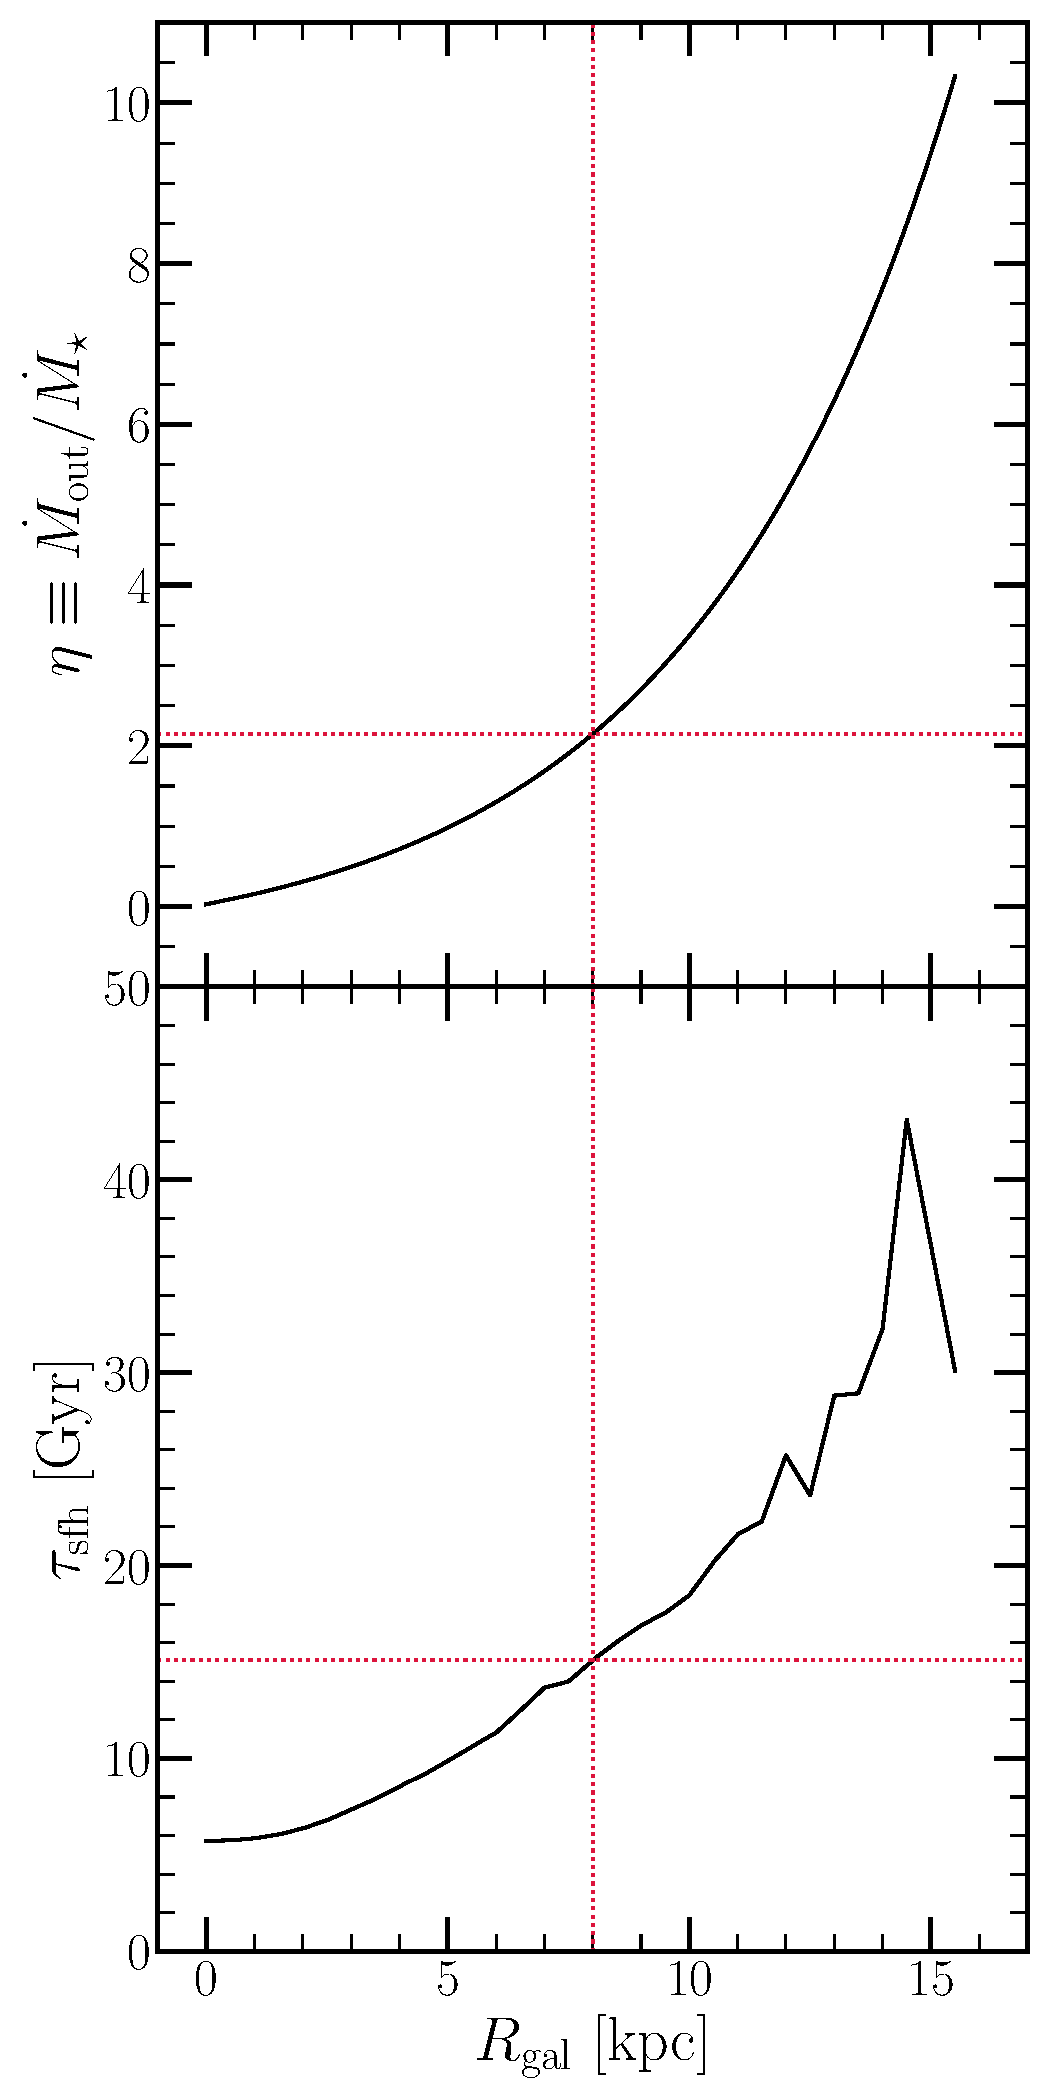
\includegraphics[scale = 0.45]{eta_tau_sfh.pdf} 
\caption{\textbf{Top}: Our implemented scaling of the mass loading factor 
$\eta$~with Galactocentric radius (black) as defined by equation 
\refp{eq:eta}.~\textbf{Bottom}: The e-folding timescales of the star formation 
histories of our model galaxies (black). These values come from a fit to the 
$\Sigma_\star$-age relation in bins of $R/R_\text{e}$ for~$10^{10.5}$~- 
$10^{11}$~M$_\odot$~Sa/Sb Hubble type spiral galaxies as reported by 
\citet[][see discussion in~\S~\ref{sec:methods:sfhs}]{Sanchez2020}. The 
horizontal and vertical red dashed lines in both panels highlight a mass 
loading factor of~$\eta \approx$ 2.15 and a star formation timescale of 
$\tau_\text{sfh} \approx$ 15 Gyr at an assumed radius of the sun of 
$R_\odot$ = 8 kpc. 
} 
\label{fig:eta_tau_sfh} 
\end{figure} 

\begin{itemize} 
	\item Both AGB star enrichment and the recycling of previously produced 
	nucleosynthetic material in this paper proceed as they did in 
	\citet{Johnson2020}, with the caveat that the mass is added to the annulus 
	that a stellar population is in at a given time, which may or may not be 
	the annulus it was born in.~\texttt{VICE} in its current version forces an 
	AGB enrichment channel in all models; for this reason, it is also included 
	in our models here, for which we adopt the yields sampled on a table of 
	initial stellar mass and metallicity from~\citet{Cristallo2011}. However, 
	the AGB star yields of O and Fe are negligible compared to their supernova
	yields. 

	\item While we make use of these new simulation features in~\texttt{VICE} 
	here, it includes a number of useful features not relevant to the current 
	paper (e.g. CCSN yield calculations using built-in tables from supernova 
	studies, z-dependent CCSN and SN Ia yields, user-constructed AGB yields as 
	functions of stellar mass and metallicity, the exchange of gas between 
	zones in a multi-zone model). {\color{red} Potentially move these 
	statements to the conclusions section near the end, where it's already 
	mentioned that~\texttt{VICE} is publicly available. } 
\end{itemize} 

\subsection{Star Formation Histories} 
\label{sec:methods:sfhs} 

% fig 4 
\begin{figure*} 
\centering 
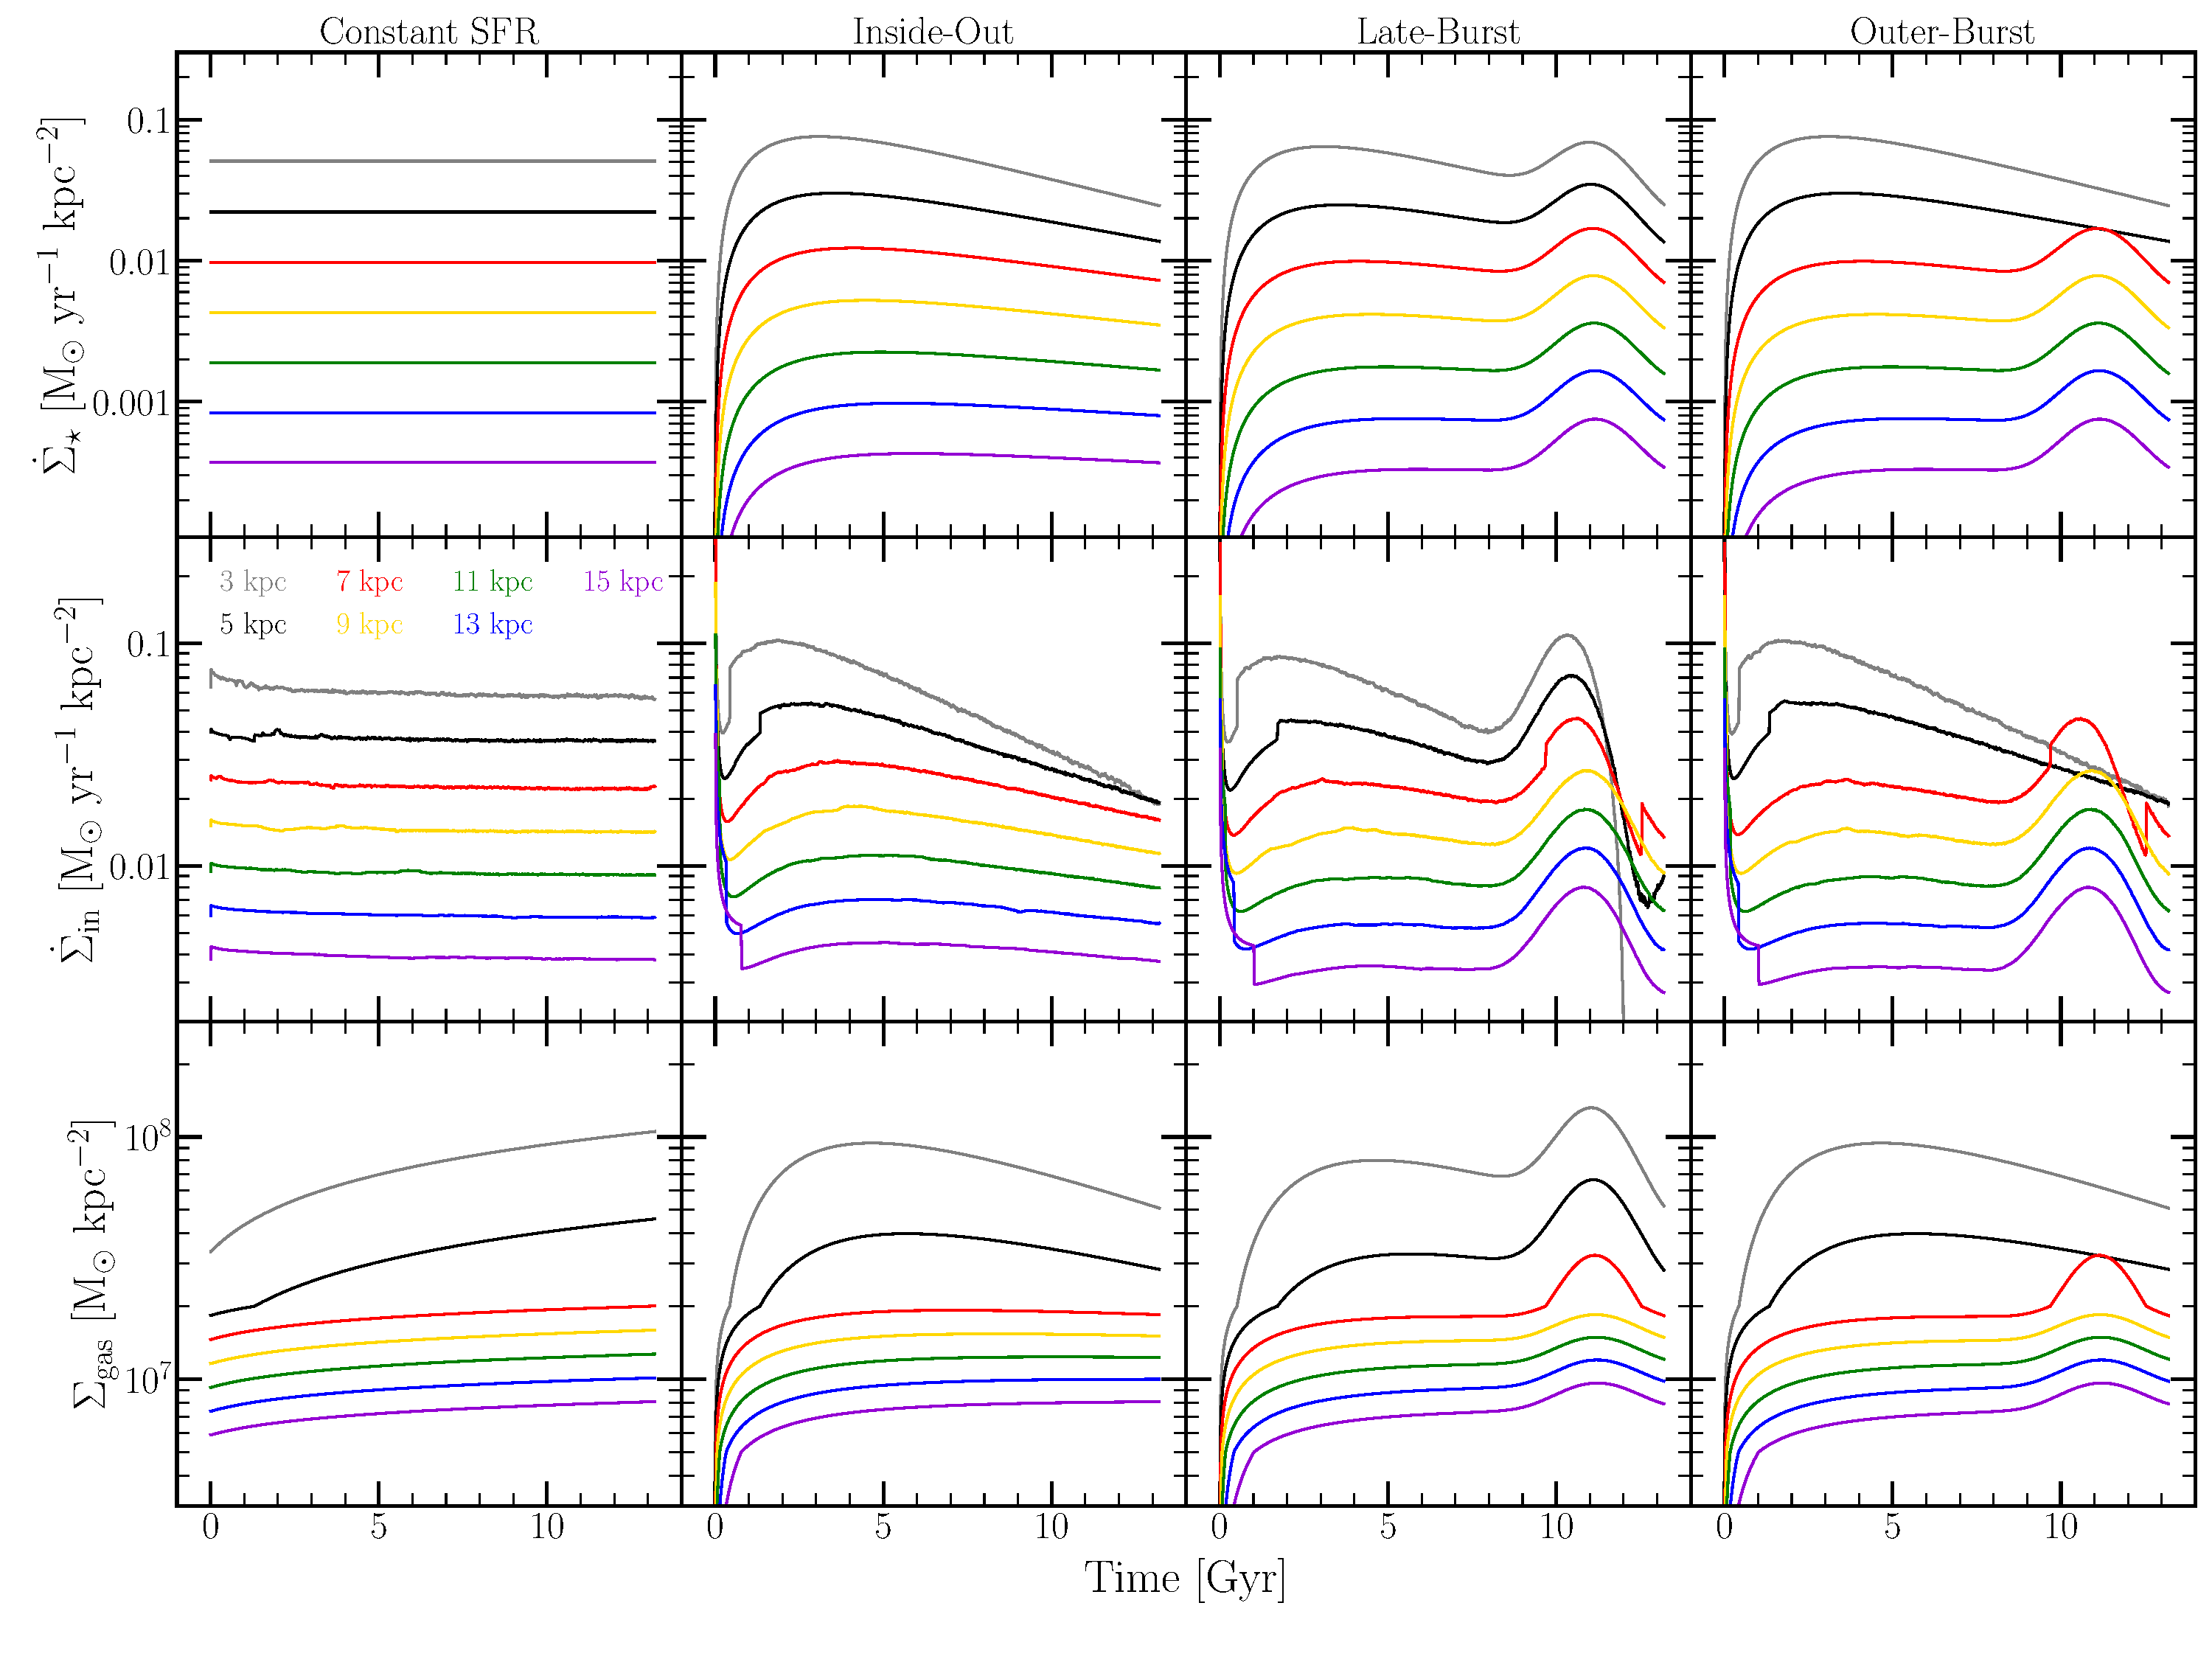
\includegraphics[scale = 0.32]{evol.pdf} 
\caption{The surface densities of star formation $\dot{\Sigma}_\star$ (top 
row), infall $\dot{\Sigma}_\text{in}$ (middle row), and gas $\Sigma_\text{g}$ 
(bottom row) as functions of simulation time for our four fiducial SFHs: 
constant (far left), inside-out (left middle), late-burst (right-middle), 
and outer-burst (far right). We plot curves for the annuli whose inner radii 
are 3 kpc (grey), 5 kpc (black), 7 kpc (red), 9 kpc (yellow), 11 kpc (green), 
13 kpc (blue), and 15 kpc (purple) (see equations~\refp{eq:constant_sfh}, 
\refp{eq:insideout_sfh},~\refp{eq:lateburst_sfh}, and~\refp{eq:outerburst_sfh} 
for the mathematical definition of each SFH). } 
\label{fig:evol} 
\end{figure*} 

\begin{itemize} 
	\item \texttt{VICE}'s simulations runs in either infall, star formation, or 
	gas mode, referring simply to which component of the evolutionary history 
	the user has specified. The fiducial starburst models presented in 
	\citet{Johnson2020} ran in infall mode, but here we run things in star 
	formation mode, since we are after specific forms for the star formation 
	histories of our models. This means that changing our assumptions about the 
	star formation law described in~\S~\ref{sec:methods:sfe} would not change 
	the star formation rate, but would change the surface density of gas at 
	each timestep, and thus also the implied infall rates. 

	\item Appendix~\ref{sec:normalize_sfh} presents justification of how we 
	normalize the parameters of our star formation histories to produce a 
	realistic model Galaxy at the end of the simulation. In short, it takes in 
	a unitless description of the time-dependence of the SFH at a given 
	Galactocentric radius, denoted $f(t|R_\text{gal})$, and a unitless 
	description of the radial dependence of the present-day stellar surface 
	density, denoted $g(R_\text{gal})$. In short, we integrate 
	$f(t|R_\text{gal})$ with time for each annulus, assuming $R_\text{gal}$ to 
	correspond to the centre of the zone, and attach a prefactor to 
	$f(t|R_\text{gal})$ at each $R_\text{gal}$ such that the desired gradient 
	is achieved with a total stellar mass similar to that of the Milky Way. 
	This procedure neglects the impact of radial migration, assuming that it 
	does not significantly alter the form of $g(R_\text{gal})$. We demonstrate 
	that these assumptions hold in~\S 
	\ref{sec:methods:surface_density_gradient}, in which we also detail our 
	adopted form of $g(R_\text{gal})$. As long as this assumption is not 
	violated, the equation derived in Appendix~\ref{sec:normalize_sfh} can be 
	used to normalize the parameters of future models of spiral galaxies. 

	\item We present four fiducial SFHs, which we dub ``constant'', 
	``inside-out'', ``late-burst'', and ``outer-burst''. They're defined as 
	follows: 
	\begin{itemize} 
		\item \textbf{Constant}: The SFH at a given radius is time-independent. 
		\begin{equation} 
		f_\text{C}(t|R_\text{gal}) = 1 
		\label{eq:constant_sfh} 
		\end{equation} 
		This case is of particular theoretical interest because it quantifies 
		the effect of ongoing with star formation with radial migration, and 
		no additional effects. 

		\item \textbf{Inside-Out}: 
		\begin{equation} 
		f_\text{IO}(t|R_\text{gal}) = (1 - e^{-t/\tau_\text{rise}})
		e^{-t/\tau_\text{sfh}} 
		\label{eq:insideout_sfh} 
		\end{equation} 
		We adopt this scenario over the traditional linear-times-exponential 
		form of $f(t|R_\text{gal})~\sim~te^{-t/\tau_\text{sfh}}$, because the 
		latter does not offer control over the position of the maximum. The 
		form we adopt has a maximum near $\tau_\text{rise}$, for which we adopt 
		a value 2 Gyr everywhere in this paper. We find that this produces a 
		peak in star formation at lookback times of~$\sim$10 Gyr, corresponding 
		to a redshift of~$z \approx$~2, which is around cosmic high noon. In 
		this paper $\tau_\text{sfh}$ is a function of $R_\text{gal}$ here, and 
		we discuss it briefly in a few paragraphs. 

		\item \textbf{Late-Burst}: An inside-out SFH with a gaussian describing 
		a starburst. 
		\begin{equation} 
		f_\text{LB}(t|R_\text{gal}) = f_\text{IO}(t|R_\text{gal}) 
		(1 + A_\text{b}e^{-(t - t_\text{b})^2/2\sigma_\text{b}^2}) 
		\label{eq:lateburst_sfh} 
		\end{equation} 
		$A_\text{b}$ is a dimensionless parameter describing the strength of 
		the starburst, $t_\text{b}$ is the time of the local maximum in the SFH 
		during the burst, and $\sigma_\text{b}$ is the width of the gaussian 
		describing it. Loosely motivated by the findings of~\citet{Isern2019} 
		and~\citet{Mor2019}. Here we take $A_\text{b}$ = 1.5, $t_\text{b}$ = 
		10.2 Gyr, and $\sigma_\text{b}$ = 1 Gyr. 

		\item \textbf{Outer-Burst}: A variation of the late-burst model in 
		which only $R_\text{gal}\geq$ 6 kpc experience the starburst. Loosely 
		motivated by findings of~\citet{Vincenzo2020} where a hydrodynamical 
		simulation of a Milky Way-like galaxy showed radially dependent 
		infall. 
		\begin{equation} 
		f_\text{OB}(t|R_\text{gal}) = \begin{cases} 
		f_\text{IO}(t|R_\text{gal}) & (R_\text{gal}~<~\text{6 kpc}) \\ 
		f_\text{LB}(t|R_\text{gal}) & (R_\text{gal}~\geq~\text{6 kpc}) 
		\end{cases} 
		\label{eq:outerburst_sfh} 
		\end{equation} 

		\item Although we do not investigate it here, an investigation into the 
		impact of more episodic star formation histories would be an 
		interesting extension of this paper. For example,~\texttt{VICE} has all 
		of the necessary features to handle models in which major episodes of 
		star formation coincide with the close passages of the Sagittarius 
		dwarf~\citep[e.g.][]{RuizLara2020}. 
	\end{itemize} 

	\item Derive e-folding timescales of star formation $\tau_\text{sfh}$ 
	from the data in~\citet{Sanchez2020}. 
	\begin{itemize} 
		\item They present the stellar surface density $\Sigma_\star$ as a 
		function of age in bins of $R/R_\text{e}$ for MaNGA galaxies, where 
		$R_\text{e}$ is the half-light radius. They conduct this analysis in 
		bins of stellar mass and for different Hubble types. Here take their 
		M$_\star$ = 10$^{10.5}$ - 10$^{11}$ M$_\odot$ bin for Sa/Sb spirals 
		(i.e. Milky Way-like galaxies). 

		\item Their reported $\Sigma_\star$-age relation is not robust enough 
		to get individual SFHs directly, but does allow the parameters of some 
		fiducial mathematical model to be fit to the population-averaged 
		trends. Assuming the $f_\text{IO}(t|R_\text{gal})$ form, we 
		simultaneously fit the normalization and the e-folding timescale 
		$\tau_\text{sfh}$ to these data. Although the normalization is 
		irrelevant to our simulations and determined via the method outlined 
		in Appendix~\ref{sec:normalize_sfh}, we adopt the resulting 
		$\tau_\text{sfh}$-$R_\text{gal}$ relation in our models. Results are 
		shown in Fig.~\ref{fig:eta_tau_sfh}. 

		\item Note that the star formation timescales are long, even for the 
		solar annulus ($\tau_\text{sfh} \approx$~15 Gyr at $R_\odot$ = 8 kpc) 
		and especially for the outer galaxy. Beyond the solar annulus, SFHs are 
		nearly constant after the initial rise at early times. 

		\item With our adopted gradient (see~\S 
		\ref{sec:methods:surface_density_gradient}, we know the present-day 
		half-mass radius to be very near 4 kpc (this is just doing a couple 
		integrals over the area of the disc). The findings of 
		\citet{Garcia-Benito2017} and~\citet{GonzalezDelgado2014} suggest that 
		half-light radii are marginally larger than half-mass radii. Based on 
		equations (4) of~\citet{GonzalezDelgado2014} relation the two for 
		circular apertures, we expect our model galaxy to have a half-light 
		radius near 5 kpc. We therefore adopt $R_\text{e}$ = 5 kpc in 
		calculating $\tau_\text{sfh}$ as a function of radius. {\color{red} 
		As I understand it, there are some results that suggest this value for 
		the Milky Way as well?} 
	\end{itemize} 

	\item Given the assumed star formation histories, the gas supply at all 
	times is known via the SFE timescale $\tau_\star$ (discussed 
	in~\S~\ref{sec:methods:sfe}). With the amount of gas lost to star formation 
	and outflows at each timestep, the infall rate is also known at all 
	timesteps. The results of all three are shown in Fig.~\ref{fig:evol}. 
\end{itemize} 

\subsection{Star Formation Efficiency} 
\label{sec:methods:sfe} 

% fig 5 
\begin{figure} 
\centering 
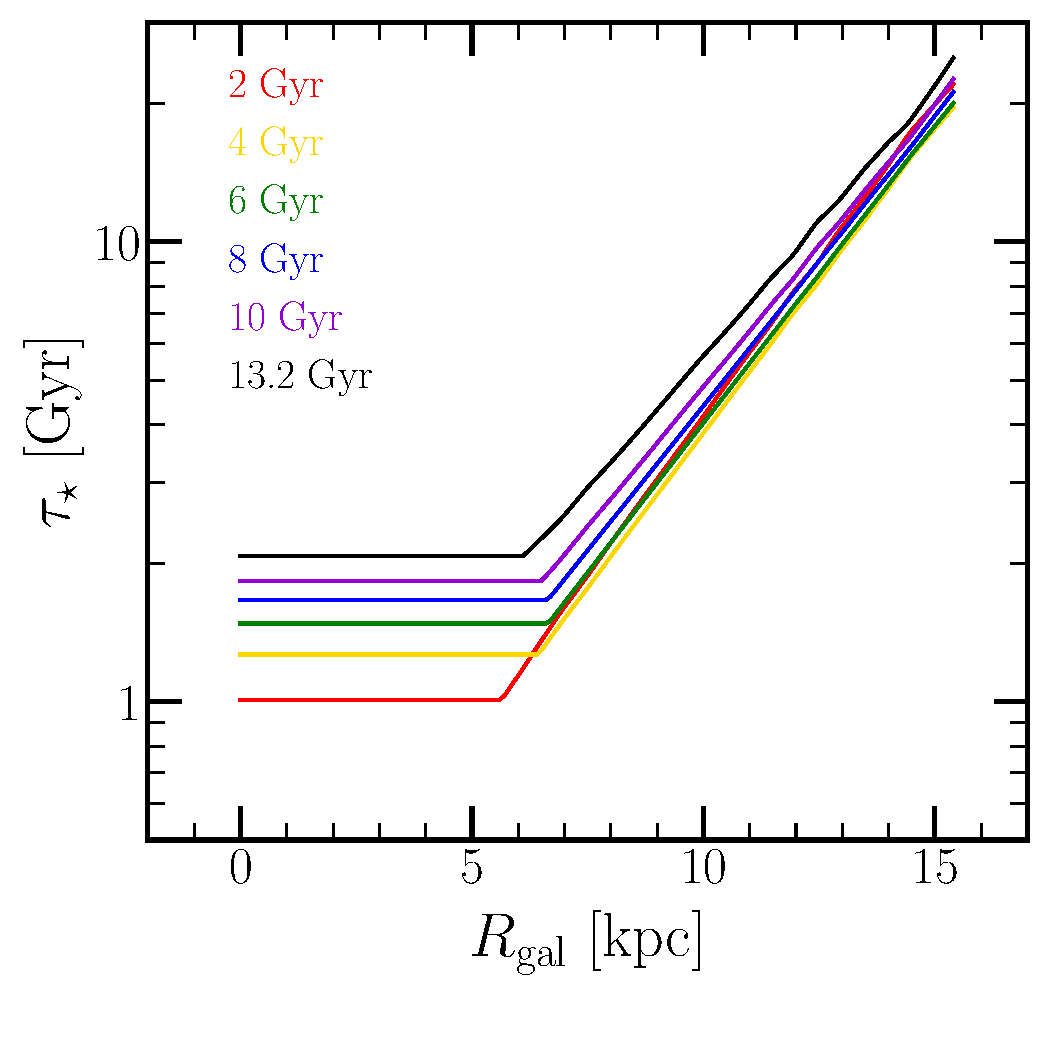
\includegraphics[scale = 0.45]{sfe.pdf} 
\caption{The star formation efficiency timescale $\tau_\star$ as a 
function of Galactocentric radius at simulation times of 2 Gyr (red), 4 Gyr 
(yellow), 6 Gyr (green), 8 Gyr (blue), 10 Gyr (purple), and 12.2 Gyr (i.e. 
the present day, black) predicted by our inside-out SFH model. }
\label{fig:sfe} 
\end{figure} 

\begin{itemize} 
	\item The term ``star formation efficiency'' (SFE) is an overloaded term in 
	the literature. In the star formation/feedback literature, it usually 
	refers to the fraction of a molecular cloud's mass which will eventually 
	be converted into stars. In the chemical evolution literature, however, it 
	usually refers to the inverse timescale relating the star formation rate 
	within some gas reservoir and the mass of the gas reservoir itself: 
	$\tau_\star \equiv \Sigma_\text{g}/\dot{\Sigma}_\star$. High (Low) 
	values of $\tau_\star$ indicate slow (fast) star formation and thus low 
	(high) SFE; when we refer to SFE here, we're referring to the definition 
	based on this timescale. In the star formation literature, this parameter 
	is often referred to as the ``depletion time.'' 

	\item Based on the findings of~\citet{Kennicutt1998}, it is common practice 
	for chemical evolution studies to implement a single power-law star 
	formation law of the form: 
	\begin{equation} 
	\dot{\Sigma}_\star \sim \Sigma_\text{g}^N 
	\end{equation} 
	where~$\dot{\Sigma}_\star$ and~$\Sigma_\text{g}$ are the surface 
	densities of star formation and ISM gas, respectively, and 
	\citet{Kennicutt1998} derive~$N = 1.4 \pm$ 0.15 relating the total 
	$\dot{\Sigma}_\star$ and $\Sigma_\text{g}$ within the disc across a 
	sample of quiescent spiral galaxies and infrared and circumnuclear 
	starbursts. However, recent studies have found evidence that much of the 
	observed scatter is physical in origin~\citep{delosReyes2019} and that 
	there are significant breaks in both the power-law index and zeropoints 
	\citep{Kennicutt2020}. Much of the uncertainty surrounding the details of 
	the star formation law is a consequence of the ongoing debate about the 
	CO-to-H$_2$ conversion factor~\citep{Kennicutt2012, Liu2015}. Although 
	\citet{Ellison2020a} demonstrate that there are significant 
	galaxy-to-galaxy variations in the star formation law, suggesting that 
	individual galaxies do not follow the population-averaged trend, 
	\citet{delosReyes2019} argue that this is still a reasonable recipe for 
	Galaxy evolution models. We adopt such a formalism here. 

	\item \citet{Krumholz2018} compare model-predicted star formation laws to 
	the observational data from~\citet{Bigiel2010} and~\citet{Leroy2013} (see 
	their Fig. 2). We find that the following by-eye fit to the power-law 
	index~$N$ is a reasonable description of the aggregate data: 
	\begin{equation} 
	N = \begin{cases} 
	1.0 & (\Sigma_\text{g} \geq \Sigma_{\text{g},2}) 
	\\ 
	3.6 & (\Sigma_{\text{g},1} \leq \Sigma_\text{g} \leq \Sigma_{\text{g},2}) 
	\\ 
	1.7 & (\Sigma_\text{g} \leq \Sigma_{\text{g},1})  
	\end{cases} 
	\label{eq:ks_law_indeces}  
	\end{equation} 
	where~$\Sigma_{\text{g},1} = 5\times10^6~\msun~\persqkpc$ and 
	$\Sigma_{\text{g},2} = 2\times10^7~\msun~\persqkpc$.  

	\item The apparent linearity of the relationship above~$\sim2\times10^7$ 
	$\msun~\persqkpc$ suggests that in this regime, star formation is 
	proceeding at the fastest possible rate, and that $\tau_\star$ = 
	$\Sigma_\text{g}/\dot{\Sigma}_\star$ = constant. The results of 
	\citet{Leroy2008, Leroy2013} and~\citet{Kennicutt2020} would suggest that 
	this is the regime in which the molecular fraction 
	$f_\text{mol} = M_{\text{H}_2} / (M_\text{HI} + M_{\text{H}_2}) \approx$ 1. 
	We therefore adopt the assumption that above $\Sigma_\text{g}$ = 
	$2\times10^7$~M$_\odot$~kpc$^{-2}$,~$\tau_\star$ reaches its minimum value, 
	and increases with decreasing~$f_\text{mol}$. We denote this value as 
	$\tau_\text{mol}$, the value of $\tau_\star$ for a gas reservoir with 
	$f_\text{mol}$ = 1. This, combined with our three-component power-law index 
	$N$ results in the following final form for our adopted star formation 
	law: 

	\begin{equation} 
	\dot{\Sigma}_\star =\begin{cases} 
	\Sigma_\text{g} \tau_\text{mol}^{-1} & (\Sigma_\text{g} \geq 
	\Sigma_{\text{g},2})  
	\\ 
	\Sigma_\text{g} \tau_\text{mol}^{-1} \left(\frac{
		\Sigma_\text{g} 
	}{
		\Sigma_{\text{g},2}
	}\right)^{2.6} & (\Sigma_{\text{g},1} \leq \Sigma_\text{g} \leq 
	\Sigma_{\text{g},2}) 
	\\ 
	\Sigma_\text{g} \tau_\text{mol}^{-1} \left(\frac{
		\Sigma_{\text{g},1} 
	}{
		\Sigma_{\text{g},2} 
	}\right)^{2.6} \left(\frac{
		\Sigma_\text{g} 
	}{
		\Sigma_{\text{g},1} 
	}\right)^{0.7} & (\Sigma_\text{g} \leq \Sigma_{\text{g},1}) 
	\end{cases} 
	\label{eq:ks_law} 
	\end{equation} 
	where we chose the power-law indeces such that this formalism is consistent 
	with equation~\refp{eq:ks_law_indeces}, and prefactors are added to ensure 
	piece-wise continuity. In implementation,~\texttt{VICE} requires the 
	$\tau_\star-\Sigma_\text{g}$ relationship when ran in infall and gas 
	modes, and the~$\tau_\star-\dot{\Sigma}_\star$ relationship when ran in 
	star formation mode. Both follow from this relationship given the 
	substitution~$\tau_\star \equiv \Sigma_\text{g}/\dot{\Sigma}_\star$. 
	\begin{itemize} 
		\item Although it is more physically motivated to use an adopted star 
		formation law to infer a star formation rate from the ISM properties at 
		a given timestep, as discussed in~\S~\ref{sec:methods:sfhs}, we are 
		using~\texttt{VICE} in star formation mode, meaning that it is 
		$\dot{\Sigma}_\star$ rather than~$\Sigma_\text{g}$ or 
		$\dot{\Sigma}_\text{in}$ which is specified~\textit{a priori}. 
		Therefore, our models are inferring~$\Sigma_\text{g}$ from 
		$\dot{\Sigma}_\star$, not the other way around. 
	\end{itemize} 

	\item Based on the observed Kennicutt-Schmidt relation at different 
	redshifts,~\citet{Tacconi2018} suggest that~$\tau_\text{mol}$ should 
	scale with redshift~$z$ and the deviation from the star forming main 
	sequence~$\delta\text{MS}$ via~$\tau_\text{mol} \propto (1 + z)^{-0.6} 
	\delta\text{MS}^{-0.44}$. We don't take into account the effect of 
	$\delta\text{MS}$ in our models, but we do investigate the redshift 
	dependence. A reasonable approximation to the $t-z$ relation out 
	to~$z \approx$~3 assuming typical~$\Lambda$CDM cosmology is given by: 
	\begin{equation} 
	\frac{t}{t_0} \approx (1 + z)^{-5/4} 
	\end{equation} 
	where $t_0$ is the present-day age of the universe, and $t$ is not 
	simulation time but the age of the universe at any given redshift. 
	Plugging this relation into the~\citet{Tacconi2018} scaling yields the 
	following time-dependence for~$\tau_\text{mol}$: 
	\begin{equation} 
	\tau_\text{mol} = \tau_{\text{mol},0}(t/t_0)^{12/25} \approx 
	\tau_{\text{mol},0}(t/t_0)^{1/2} 
	\end{equation} 
	where $\tau_{\text{mol},0}$ is simply $\tau_\text{mol}$ at the 
	present day. We generalize this formula to the following form: 
	\begin{equation} 
	\tau_\text{mol} = \tau_{\text{mol},0}(t/t_0)^\gamma 
	\label{eq:tau_mol}
	\end{equation} 
	In this paper we present simulations which adopt~$\tau_{\text{mol},0}$ 
	= 2 Gyr~\citep{Leroy2008, Leroy2013, Tacconi2018} and~$\gamma$~= 1/2 based 
	on this argument. We have also ran simulations which adopt 
	$\tau_{\text{mol},0}$ = 1 Gyr and~$\gamma$~= 0 (a time-independent 
	$\tau_{\text{mol}}$), and found similar results. 

	\item At all timesteps in our models,~$\Sigma_\text{g}$ is inferred from 
	$\dot{\Sigma}_\star$ directly from equations~\refp{eq:ks_law} and 
	\refp{eq:tau_mol}. The infall rate is subsequently calculated from the 
	amount of gas lost to new stars and outflows within a given timestep and 
	the amount of gas implied by the star formation rate at the next timestep, 
	and is assumed to be zero metallicity. 

	\item Fig.~\ref{fig:sfe} shows $\tau_\star$ as a function of $R_\text{gal}$ 
	at six different time stamps predicted by our fiducial, inside-out SFH 
	model. At~$R_\text{gal} \lesssim$6 kpc,~$\tau_\star$ is near 
	$\tau_\text{mol}$ at all times, implying a molecular fraction of unity at 
	these radii. Although this prediction is likely unrealistic ({\color{red} 
	citation?}), relaxing our assumptions about the star formation law does not 
	significantly impact our conclusions. In collecting results for this paper, 
	we investigated purely linear, purely power-law, and broken power-law star 
	formation laws, finding similar predictions in all cases. In practice we 
	find that the detailed form the star formation history and, to some extent, 
	the time-dependence of radial migration have much more power over the model 
	predictions. We interpret this as an indication that the details of the 
	star formation law are at most secondary effects in establishing the model 
	behavior. 
\end{itemize} 

\subsection{Surface Density Gradient} 
\label{sec:methods:surface_density_gradient} 

% fig 6 
\begin{figure} 
\centering 
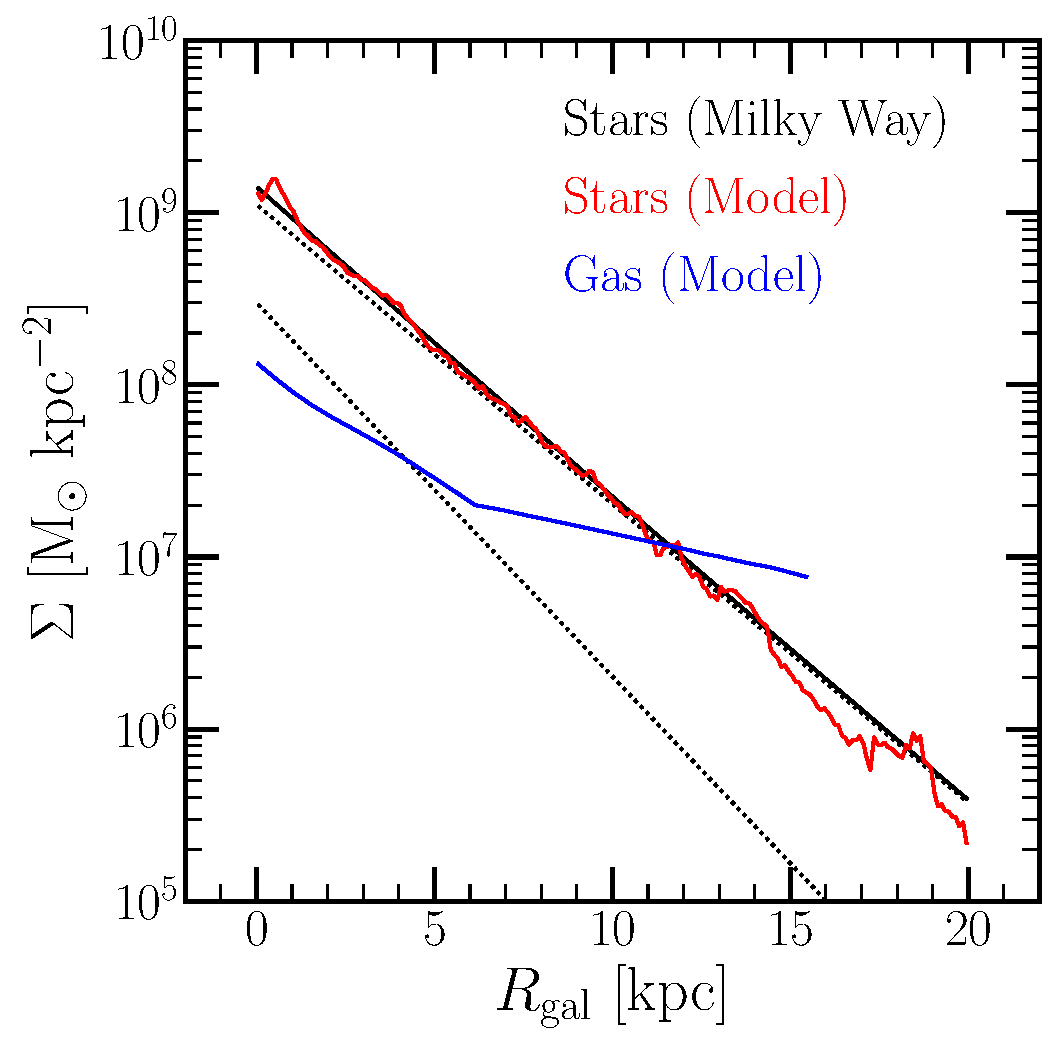
\includegraphics[scale = 0.45]{surface_density_gradient.pdf} 
\caption{The surface density of gas (blue) and stars (red) as predicted by our 
inside-out SFH model. The dotted black line with the higher normalization 
denotes a thin disc profile with scale length $R_t$ = 2.5 kpc; the other 
denotes a thick disc profile with scale length $R_T$ = 2.0 kpc, and a ratio of 
$\Sigma_T/\Sigma_t$ = 0.27 at $R_\text{gal}$ = 0. The solid black line denotes 
the sum of the two; this is the surface density gradient of the Milky Way as 
reported by~\citet{Bland-Hawthorn2016}, renormalized to imply the same total 
stellar mass within the disc. } 
\label{fig:surface_density} 
\end{figure} 

\begin{itemize} 
	\item As discussed in~\S~\ref{sec:methods:sfhs}, Appendix 
	\ref{sec:normalize_sfh} presents justification of a recipe in which we 
	select a unitless, unnormalized form describing the scaling of the 
	stellar surface density with Galactocentric radius, denoted 
	$g(R_\text{gal})$. Here we adopt the following double exponential form, 
	describing the thin and thick discs of the Milky Way: 
	\begin{equation} 
	g(R_\text{gal}) = e^{-R/R_t} + \frac{\Sigma_T}{\Sigma_t}e^{-R/R_T} 
	\end{equation} 
	where $R_t$ and $R_T$ are the scale radii of the thin and thick discs, 
	respectively, and $\Sigma_T/\Sigma_t$ is the ratio of their surface 
	densities at $R_\text{gal}$ = 0. In this paper, we adopt $R_t$ = 2.5 kpc, 
	$R_T$ = 2.0 kpc, and $\Sigma_T/\Sigma_t$ = 0.27 from the findings of 
	\citet{Bland-Hawthorn2016}. These are illustrated by the two dotted black 
	lines in Fig.~\ref{fig:surface_density}, with the solid one denoting the 
	sum of the two. Both have been re-normalized such that the integral over 
	the surface area of the model Galaxy implies a total stellar mass in 
	agreement with our adopted value. 

	\item Adopt the~\citet{Licquia2015} total stellar mass of 
	$(6.08\pm1.14)\times10^{10}~M_\odot$. We're including bulge star particles 
	in our sample of candidate analogs from~\texttt{h277}, so we model the 
	entire stellar mass as opposed to just the disc, for 
	which~\citet{Licquia2015} found $(5.17\pm1.11)\times10^{10}~M_\odot$. 
	This choice only matters in setting the overall normalization of our 
	adopted star formation histories~$\dot{\Sigma}_\star$ as a function of 
	radius and time, in turn affecting the inferred gas surface density 
	$\Sigma_\text{g}$ via our adopted star formation law (see discussion in 
	\S~\ref{sec:methods:sfe}). In short, lower (higher) stellar masses suggest 
	longer (shorter) values of~$\tau_\star$ at all times. This only impacts our 
	models insofar as our choice about the star formation law matters; as 
	discussed in~\S~\ref{sec:methods:sfe}, we find in practice that varying 
	those assumptions don't impact our conclusions. We find the same for models 
	with a different present-day stellar mass. 

	\item Surface density gradient from fiducial model with inside-out SFH, 
	plotted in Fig.~\ref{fig:surface_density} (stars in red and gas in blue). 
	Radial migration indeed didn't change the overall scaling of 
	$\Sigma_\star$ with $R_\text{gal}$ at the radii that we care about in 
	this paper (3 kpc~$\lesssim R_\text{gal} \lesssim$~15 kpc), only 
	introducing scatter. Gas disc appears to flatten at 
	$R_\text{gal}~\gtrsim$ 6 kpc; this is a consequence of our model for star 
	formation efficiency (see discussion in~\S~\ref{sec:methods:sfe}). The 
	radius at which~$\Sigma_\text{g}$ shows a break in Fig. 
	\ref{fig:surface_density} coincides with the radius at which 
	$\Sigma_\text{g}$ is low enough to transition from the 
	$\dot{\Sigma}_\star \sim \Sigma_\text{g}$ to the 
	$\dot{\Sigma}_\star \sim \Sigma_\text{g}^{3.6}$ piece of our adopted star 
	formation law. With our star formation histories specified 
	\textit{a priori}, these choices impact the radial profile of 
	$\Sigma_\text{g}$. 
\end{itemize} 

\subsection{Summary} 
\label{sec:methods:summary} 

\begin{itemize} 
	\item In summary, our fiducial model has an inside-out SFH (see~\S 
	\ref{sec:methods:sfhs}) with the star formation law as described in~\S 
	\ref{sec:methods:sfe}, radial migration the proceeds according to the 
	diffusion model (see~\S~\ref{sec:methods:migration}), and yields and 
	outflows as described in~\S~\ref{sec:methods:yields}. 

	\item We have also conducted runs with the three other SFHs, the three 
	other migration prescriptions, and the three other SFE prescriptions - a 
	total of 64 simulations, as well as a variety of other test cases. In this 
	paper, we present results wherever the model predictions are sensitive to 
	the assumptions. However, in general the differences can be understood 
	with only the variations in star formation history and the qualitative 
	notion that many stars have moved beyond their birth radius. 

	\item To ensure that resolution does not affect our results, we ran the 
	same set of models with~$n$ = 2 stellar populations per zone per 
	timestep, and found similar predictions. 
\end{itemize} 

\section{Comparison to Observations} 
\label{sec:comp_obs} 

% fig 7 
\begin{figure*} 
\centering 
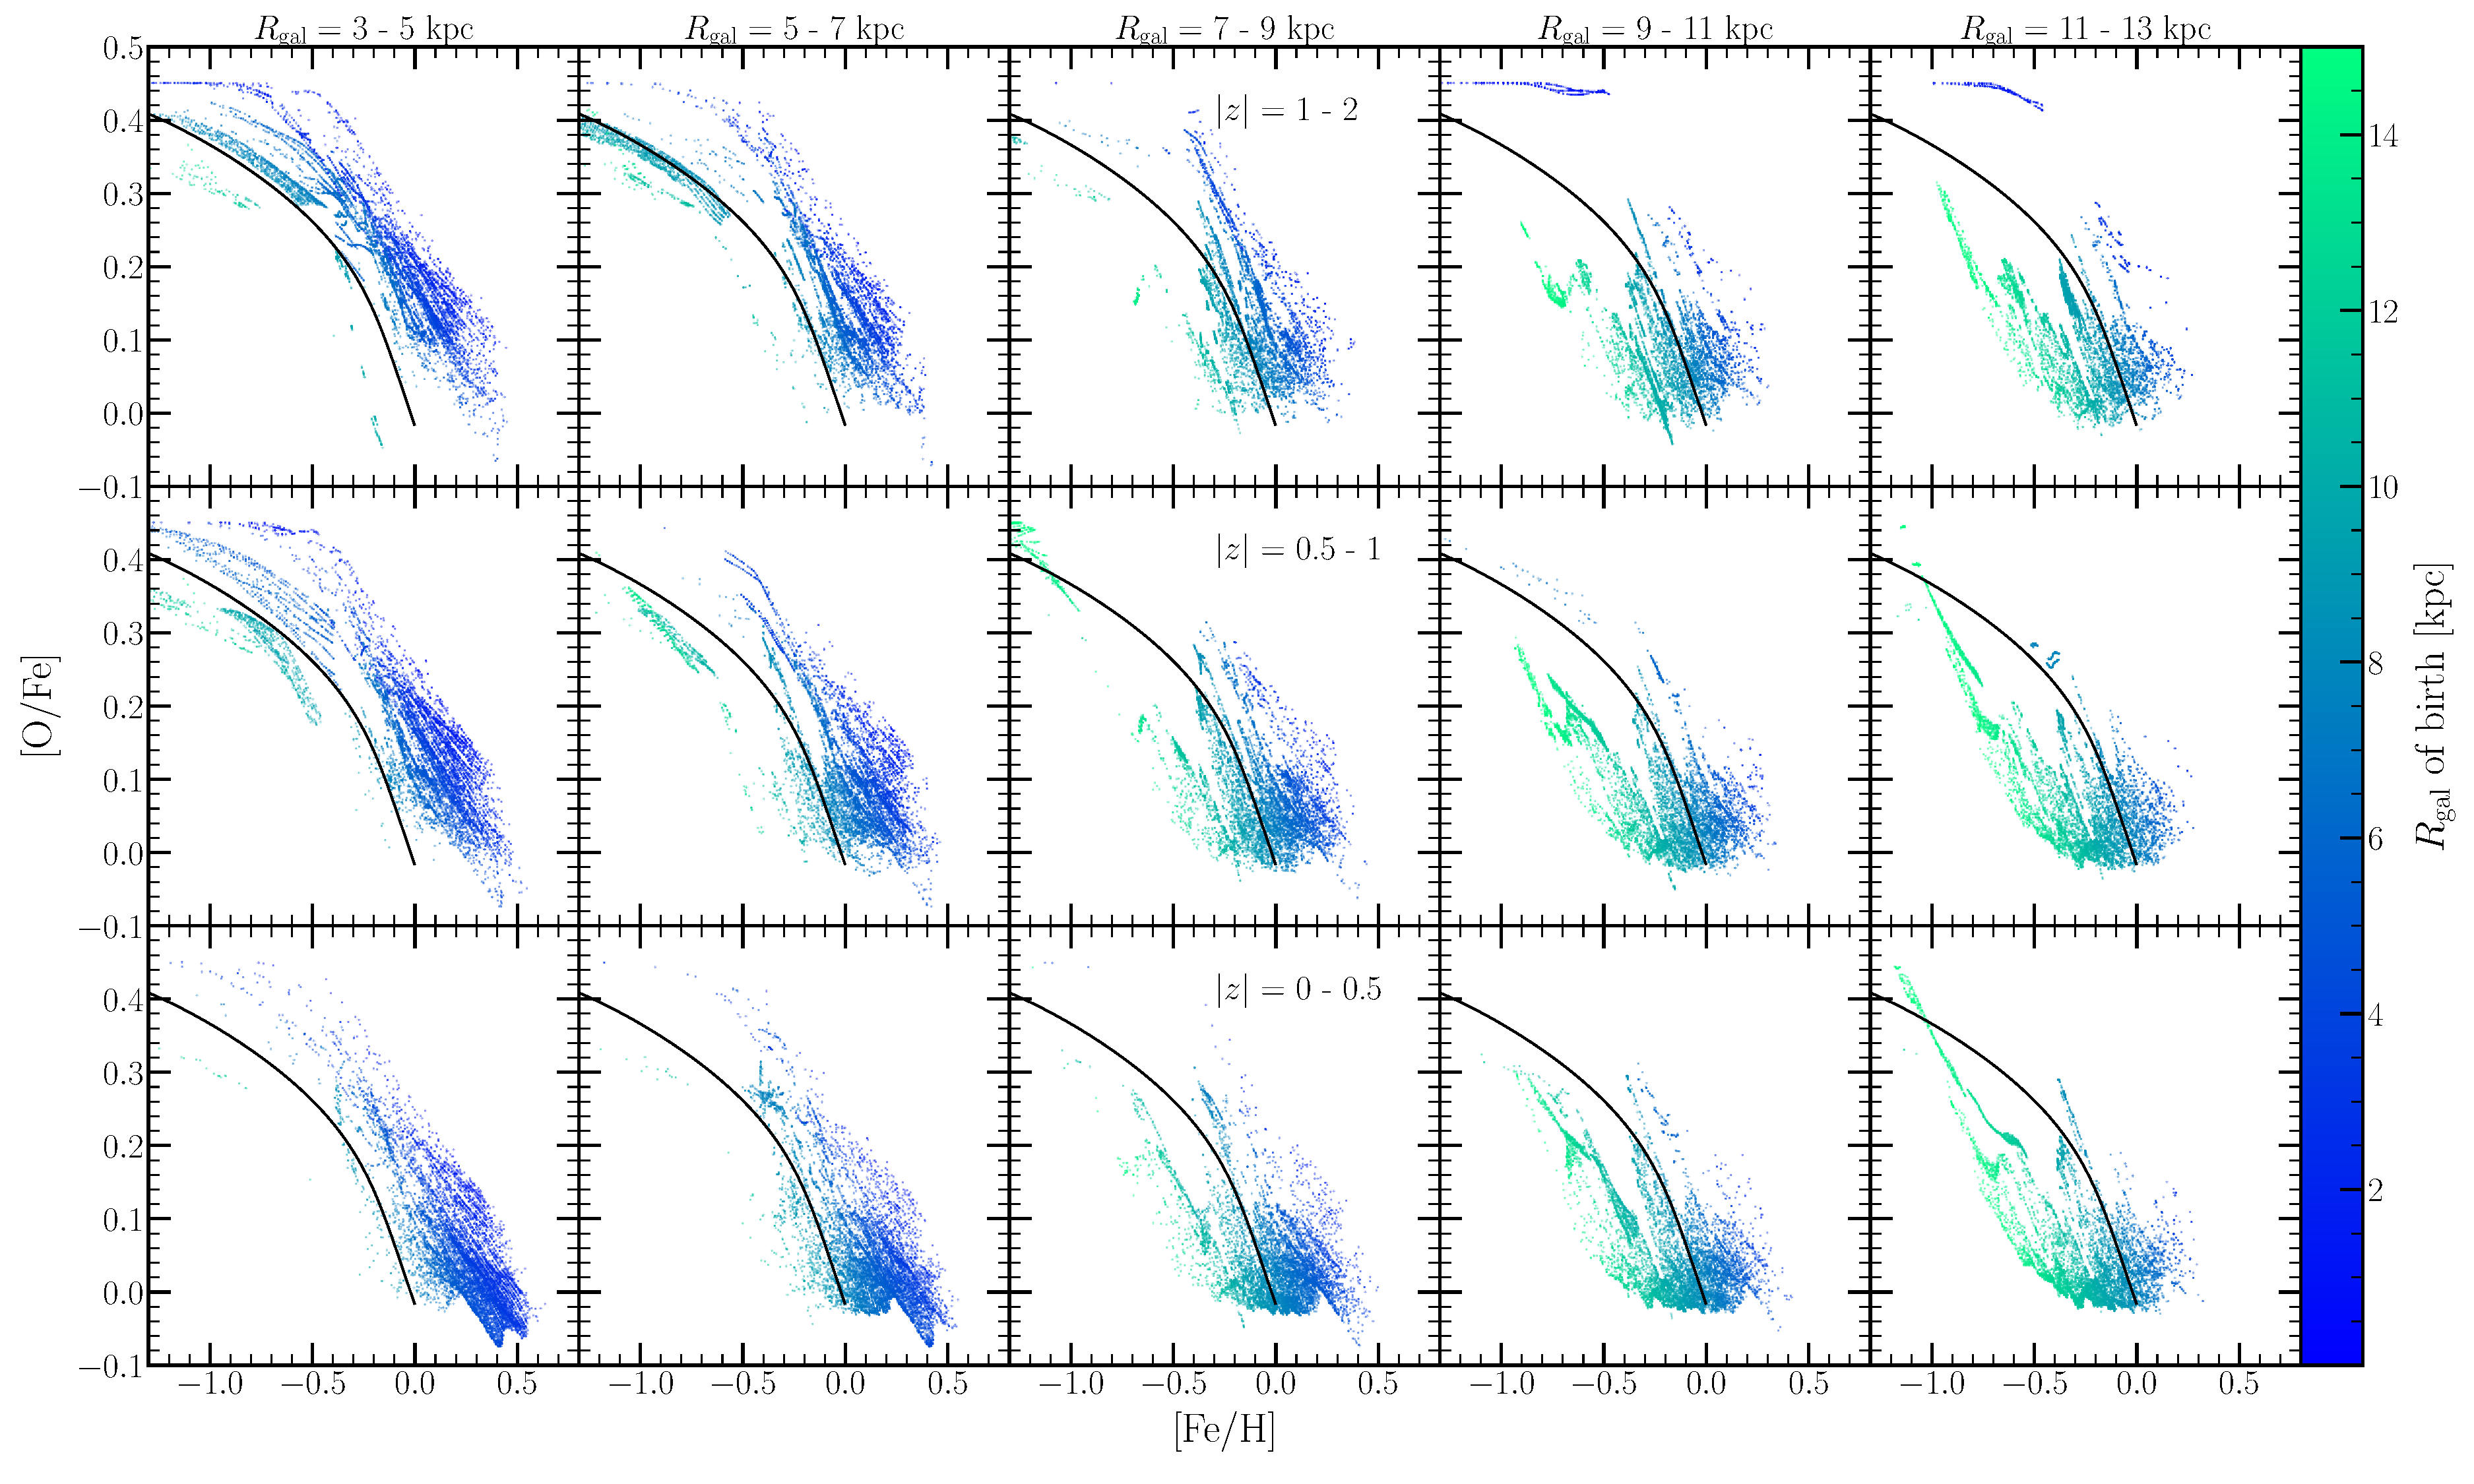
\includegraphics[scale = 0.28]{ofe_feh_densitymap.pdf} 
\caption{[O/Fe]-[Fe/H] diagrams for 15 galactic regions spanning five bins in 
$R_\text{gal}$ and~$\left|z\right|$. Each region has its own panel, with radial 
bins shown in columns denoted at the top of the figure, and with 
$\left|z\right|$ bins shown in rows denoted in text in the middle column. In 
each panel, we plot $N$ = 10,000 points sampled from our simulated 
stellar populations in each region predicted by our inside-out SFH, where the 
probability of sampling is proportional to the present-day mass of each stellar 
population. In all panels points are color-coded according to the 
Galactocentric radius of birth of the stellar population. For reference, we 
plot in a solid black line in all panels the gas-phase [O/Fe]-[Fe/H] track 
predicted by the same SFH in the $R_\text{gal}$ = 8 kpc annulus, but with the 
post-processing migration model; this curve is the same in all panels. }
\label{fig:ofe_feh_diagram} 
\end{figure*} 

% fig 8 
\begin{figure*} 
\centering 
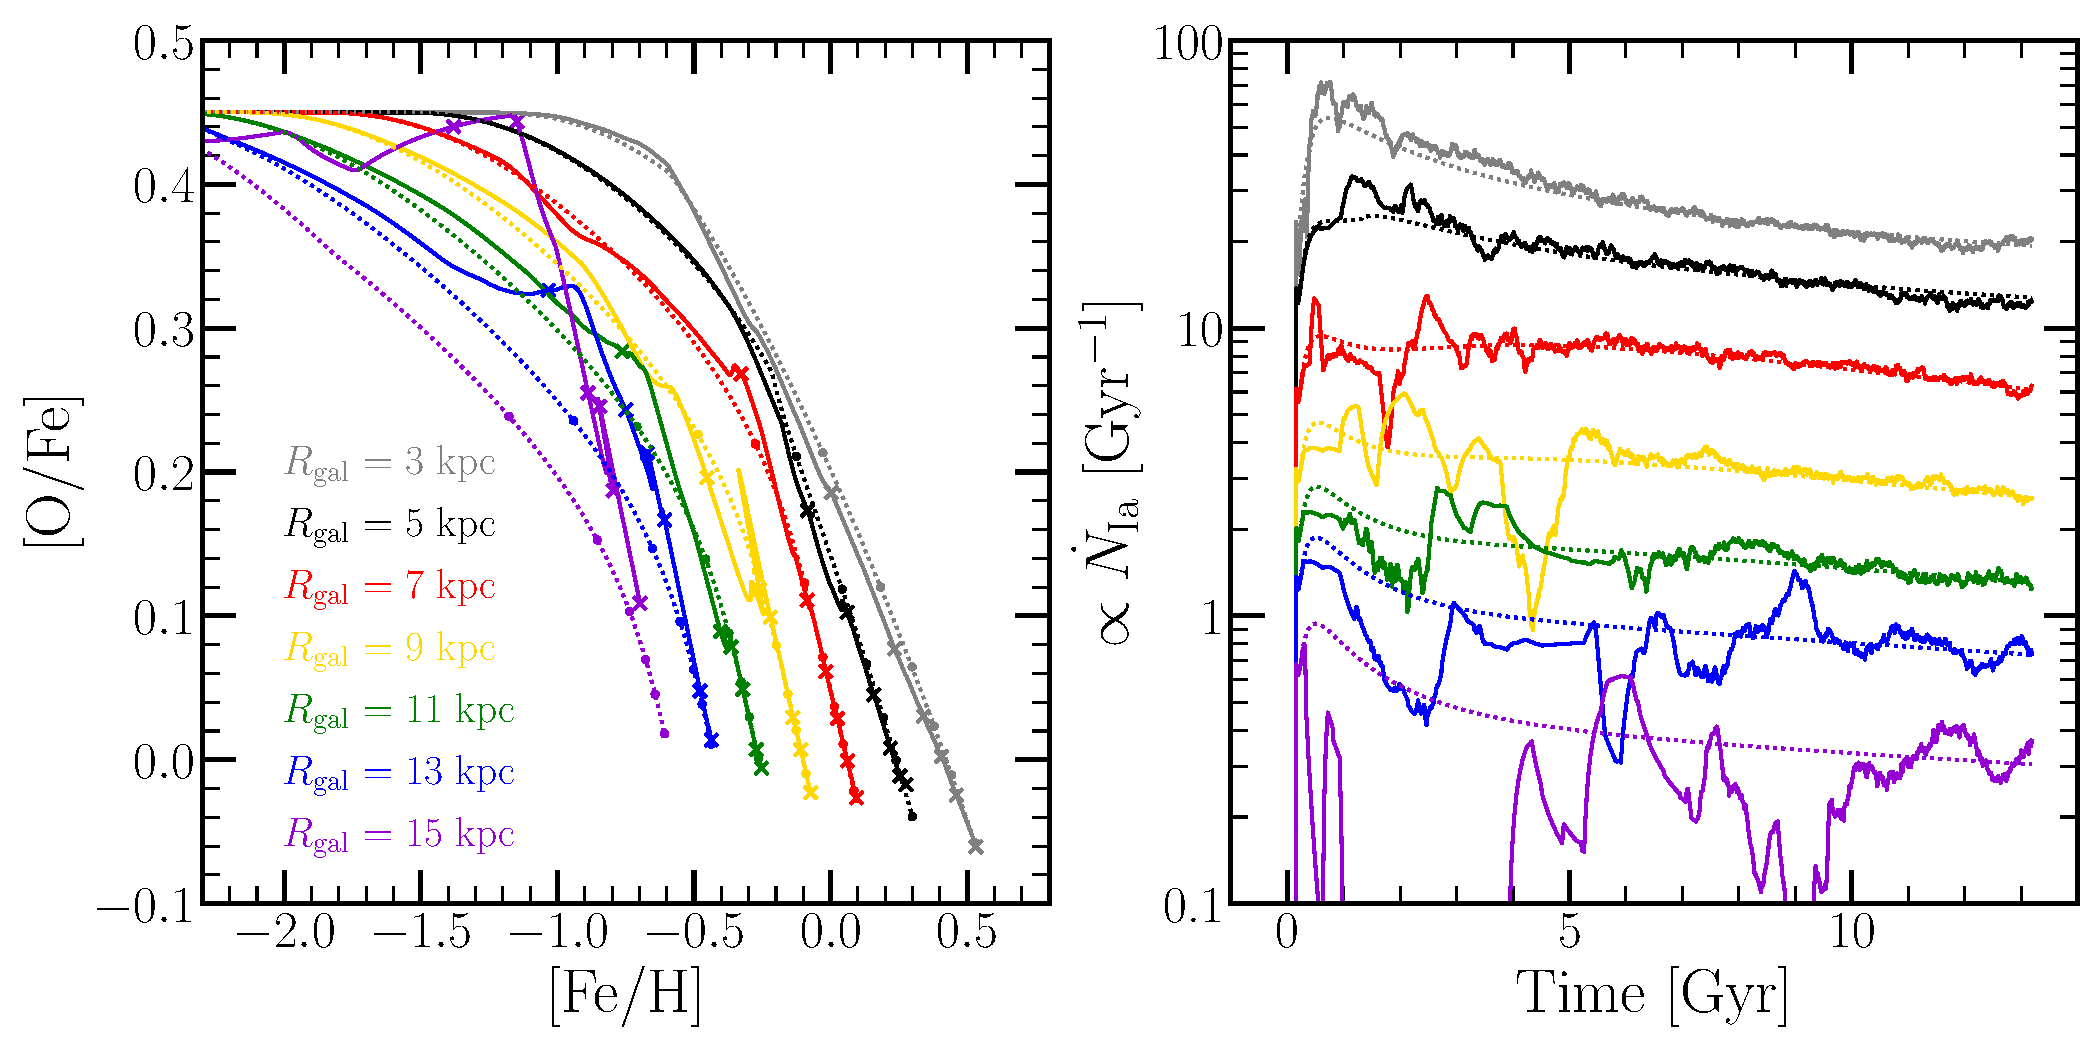
\includegraphics[scale = 0.42]{tracks.pdf} 
\caption{\textbf{Left}: Gas phase evolutionary tracks in the [O/Fe]-[Fe/H] 
plane for our inside-out SFH with either post-processing (dotted lines) or 
diffusion (solid lines) migration models. We plot tracks for seven annuli, 
color-coded according to their Galactocentric radius and denoted by the legend 
in the lower-left. We mark simulation times of 2, 4, 6, 8, 10, and 12.2 Gyr in 
X's for the diffusion model and points for the post-processing model. 
\textbf{Right}: As a function of simulation time, a proxy for the SN Ia rate 
using the total time-derivative of the Fe mass in a given annulus, calculated 
by subtracting the contribution from recycling and CCSN enrichment and adding 
back that lost to star formation and outflows. We show these rates for the 
same annuli as in the left-hand panel, multiplying them by various prefactors 
to improve clarity. } 
\label{fig:tracks} 
\end{figure*} 

\begin{itemize} 
	\item Fig.~\ref{fig:ofe_feh_diagram} shows a scatter plot of 10,000 
	randomly sampled stellar populations in five bins of $R_\text{gal}$ and 
	three bins of $\left|z\right|$ ($R_\text{gal}$ = 3 - 5 kpc, 5 - 7 kpc, 
	7 - 9 kpc, 9 - 11 kpc, and 11 - 13 kpc; $\left|z\right|$ = 0 - 0.5 kpc, 
	0.5 - 1 kpc, and 1 - 2 kpc). These are the same bins and same scheme for 
	organizing the panels as in Fig. 4 of~\citet{Hayden2015}. 

	\item The width of the low-$\alpha$ sequence predicted by the model comes 
	from radial migration. Though this wouldn't occur without radial migration, 
	our models by construction predict an ISM which spends most of its time 
	near the equilibrium abundance along the low-$\alpha$ sequence with a 
	built-in metallicity gradient. For this reason, it's only natural that our 
	models predict this to be the case, although nonetheless it is in good 
	agreement with~\citet{Schoenrich2009} and~\citet{Nidever2014}. 

	\item The low-$\alpha$ sequence shifts from a high [Fe/H] locus at small 
	$R_\text{gal}$ to low [Fe/H] at high~$R_\text{gal}$, in agreement with the 
	observed distributions in APOGEE presented in~\citet{Hayden2015}. 

	\item High-$\alpha$ stars are most prevalent at low~$R_\text{gal}$ and 
	high~$\left|z\right|$, and conversely for the low-$\alpha$ stars, also 
	in agreement with~\citet{Hayden2015}. 
	\begin{itemize} 
		\item Similar results are found for different SFHs. This suggests that 
		this observed result is a natural consequence of stellar migration. 

		\item Only minor difference worth noting is that the starburst models 
		predict a slightly higher characteristic [O/Fe] ($\sim$+0.1) for the 
		low-$\alpha$ sequence. This is a natural consequence of the starburst 
		producing young,~$\alpha$-enhanced stars~\citep{Johnson2020}. 
	\end{itemize} 
\end{itemize} 

\subsection{Abundance Gradients} 
\label{sec:comp_obs:metallicity_gradient} 

\begin{itemize} 

	\item Left-hand panel of Fig.~\ref{fig:tracks} compares the tracks 
	predicted by our fiducial, inside-out SFH assuming diffusion migration 
	(solid lines) versus post-processing (dotted lines) for the gas-phase of a 
	handful of radii denoted by the legend. Predicted [O/Fe]-[Fe/H] tracks for 
	the diffusion model show significant deviations from the post-processing 
	model. We demonstrate here that this is due to variability in the SN Ia 
	rate induced by the time-dependent radial migration of the diffusion 
	model. Simulation times of 2, 4, 6, 8, 10, and 12.2 Gyr shown in points 
	and X's for the two models. 

	\begin{itemize} 
		\item For each zone,~\texttt{VICE} provides in its outputs the rates 
		of infall and star formation, the mass of the ISM, and the relevant 
		abundance information for each element along with the associated 
		MDFs at the final timestep. To determine the SN Ia rates, we therefore 
		have to approximate from the output. 

		\item From the~\texttt{VICE} outputs of our models, we extract a 
		proxy for the SN Ia rate by isolating the contribution from SNe Ia to 
		the time derivative of the Fe mass. The total time derivative can be 
		obtained by the difference in Fe mass across two timesteps; then 
		subtracting the contribution from CCSNe and approximately correcting 
		for recycling yields an estimate of~$\dot{M}_\text{Fe}^\text{Ia}$. 

		\item This proxy is plotted against simulation time in the right-hand 
		panel of Fig.~\ref{fig:tracks} for the same annuli as in the left-hand 
		panel, with multiplicative factors added for visual clarity, diffusion 
		model again shown in solid lines, post-processing in dotted lines. 
		Whenever and wherever there is a deficit in SN Ia events relative to 
		the post-processing model, the diffusion model tends toward higher 
		[O/Fe] values than the post-processing scenario. Conversely, lower 
		[O/Fe] for an excess in SN Ia events. 

		\item SN Ia rates show high-amplitude variability on Gyr timescales, 
		with low-amplitude white-noise on shorter timescales, potentially 
		introduced at least in part by our discretization of the disc into 
		annuli and the evolution into timesteps. The log-scaled y-axis makes 
		it clear that the fractional amplitude is higher near the outskirts 
		of the disc. This makes physical sense, because the stellar number 
		density is much lower there, and as such would be much more 
		susceptible to sampling noise - that is, a single star migrating 
		has a larger fractional impact on the stellar density and thus the 
		supernova rates at large radii than small radii. 

		\item Fluctuations in the SN Ia rate at these amplitudes can be 
		understood through a comparison of the timescales associated with 
		orbital migration and SN Ia event delays. In the top panels of Fig. 
		\ref{fig:h277_decomposition}, we note that the distribution of 
		$R_\text{Final}$ is significantly more peaked in the 0 - 2 Gyr age bin 
		than for older stars. Despite this, the value of the PDF in all radial 
		bins implies~$\sim$40-50\% of~\texttt{h277} star particles migrated 
		significantly beyond their birth radius by the time they were 2 Gyr 
		old. Though we adopt a different form in detail here, the SN Ia DTD is 
		to order of magnitude a $t^{-1}$ power-law with a minimum delay of 
		$\sim$100 Myr~\citep{Maoz2012, Maoz2017}. With this DTD, there are the 
		same number of SN Ia events with delay-times between 100 Myr and 1 Gyr 
		as between 1 Gyr and 10 Gyr. Combining these two pieces of information 
		would suggest that a significant fraction of SN Ia progenitors migrate 
		significantly beyond their birth radius. That is, while radial 
		migration is often described as a slow process, so is the SN Ia DTD due 
		to its long tail. With this realization, variability in the SN Ia rate 
		at the levels seen in our models is not surprising. 
	\end{itemize} 

	\item This is proof of concept that radial migration of nucleosynthetic 
	yields can occur alongside stellar migration for delayed sources. In 
	general, the characteristic delay-time for SN Ia events is~$\sim$1 Gyr, and 
	stellar migration is proceeding on similar timescales in our models. In 
	principle, it is reasonable to expect similar effects for s-process 
	elements like carbon, nitrogen, strontium, yttrium, zirconium, etc. which 
	are produced in AGB stars and thus have similar characteristic delay-times, 
	though we do not investigate the impact for these elements here. 

	\item What we really learn from this investigation is that when stellar 
	migration is taken into account, tracks are not simple functions. To first 
	order, they are characterized by the late-time equilibrium abundance and 
	the value of~$\tau_\star$ setting the position of the ``knee'' 
	\citep{Weinberg2017}, though migration causes noticeable variations, 

	\item Demonstrate in~\S~\ref{sec:comp_obs:age_alpha} that this is a means 
	with which to form $\alpha$-rich and $\alpha$-poor stars - or rather 
	Fe-poor and Fe-rich, respectively. 
\end{itemize} 

% fig 9 
\begin{figure*} 
\centering 
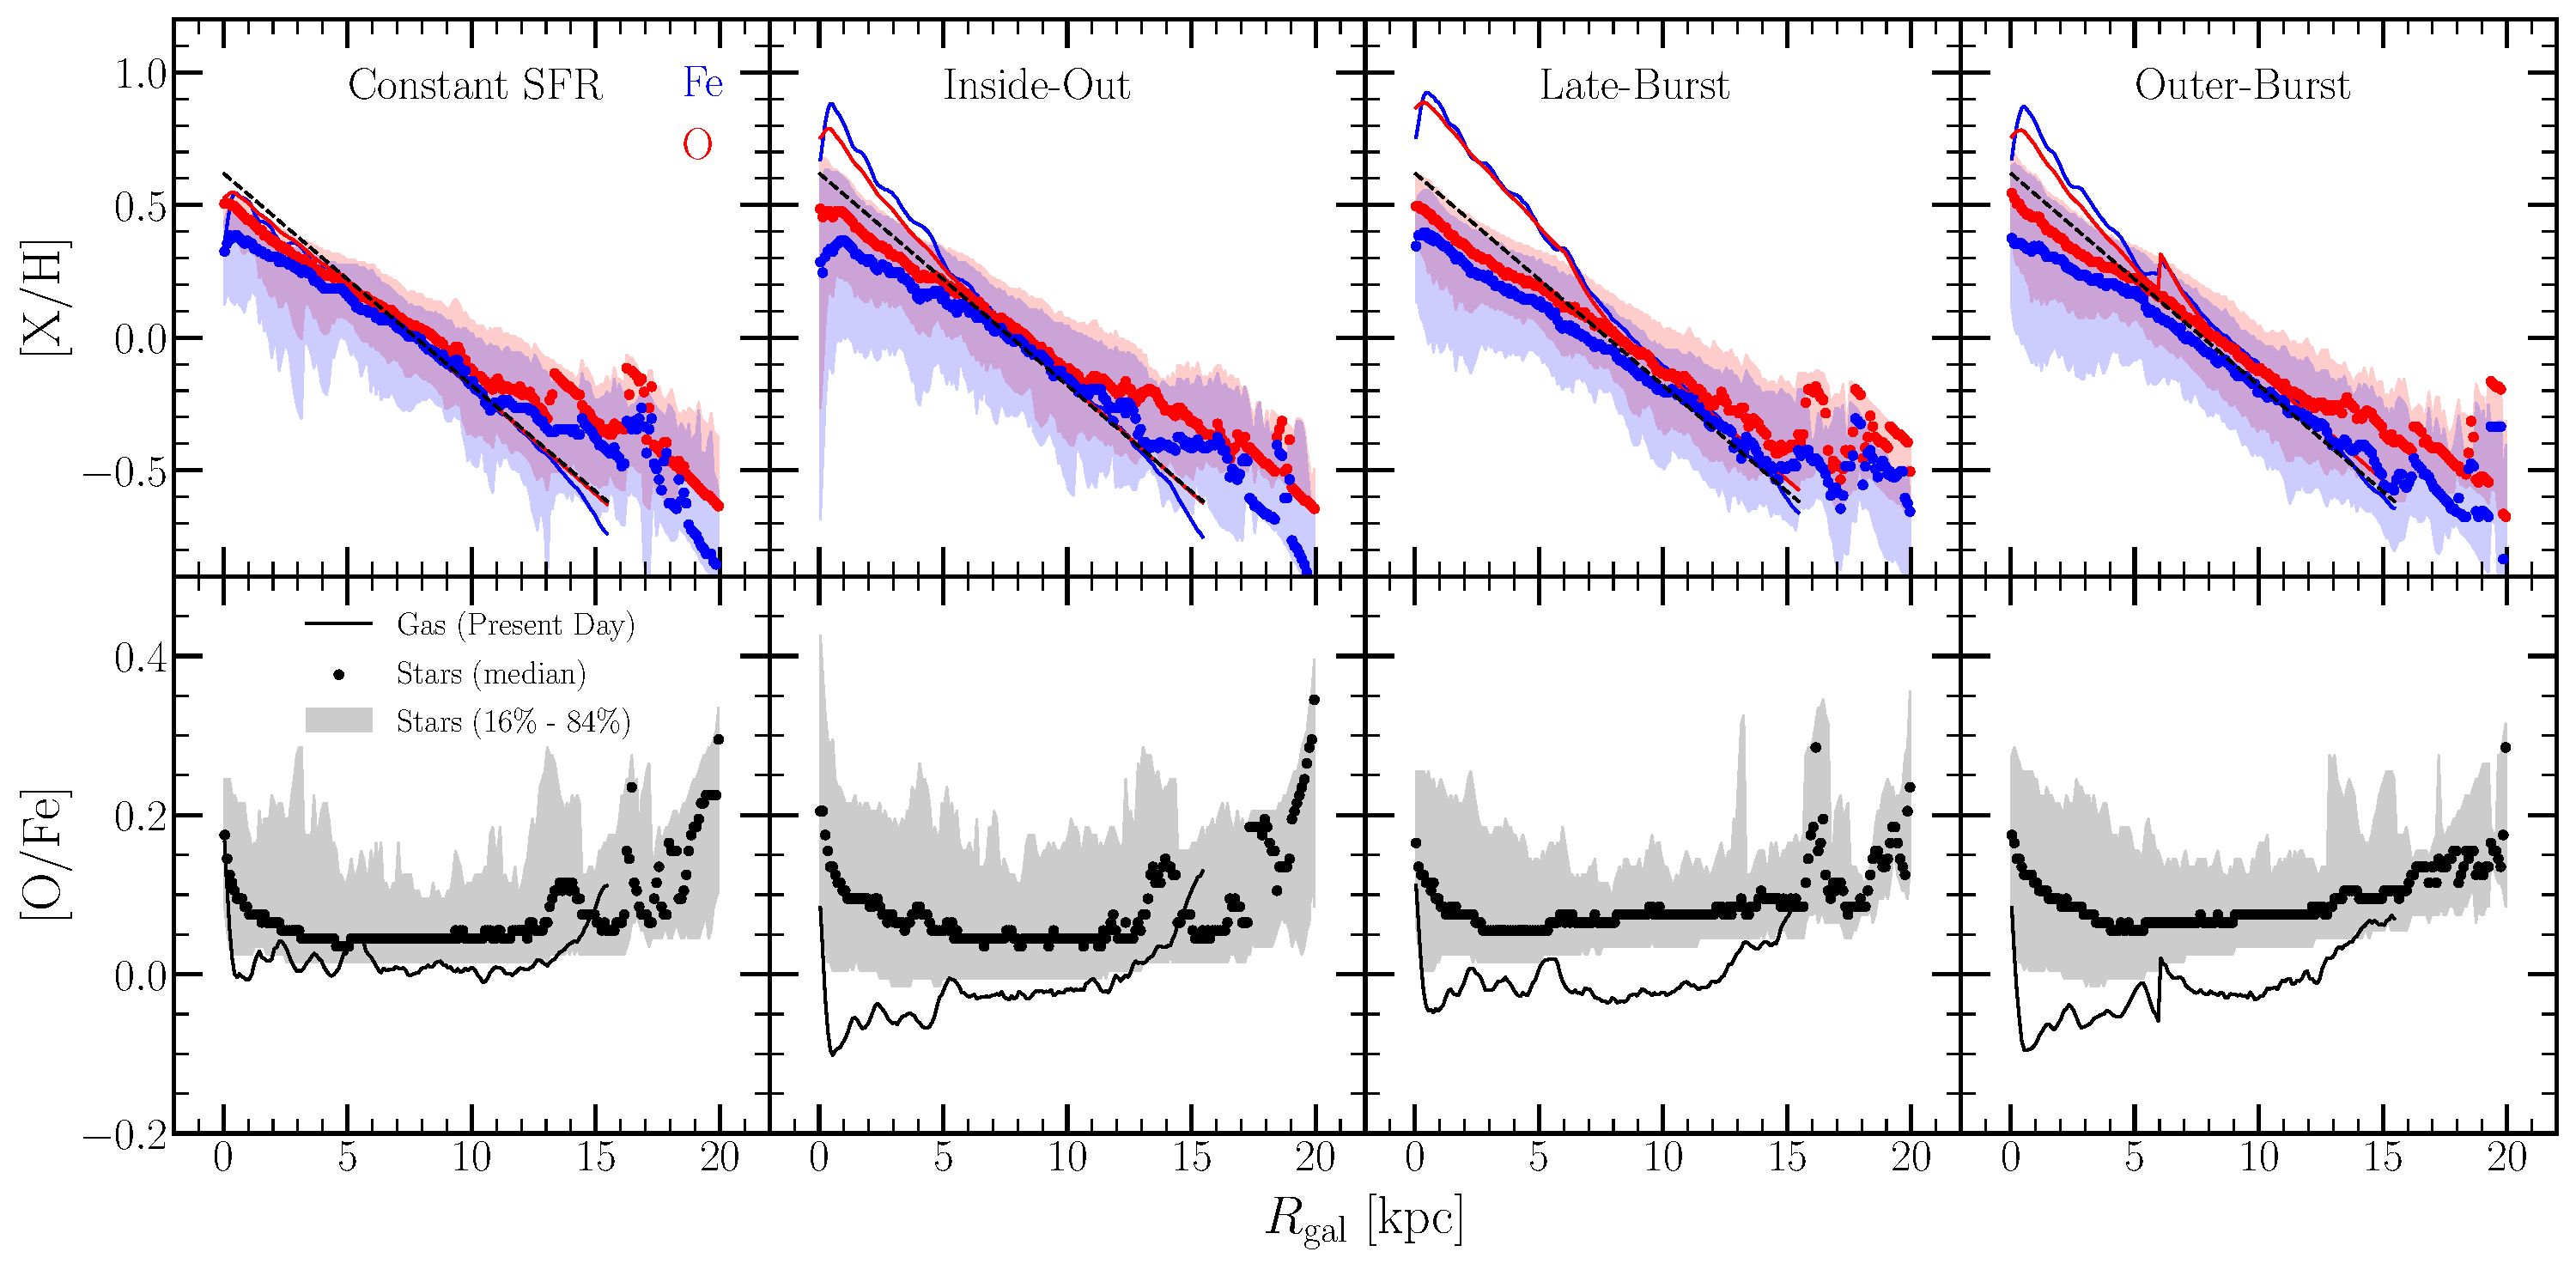
\includegraphics[scale = 0.32]{metallicity_gradient.pdf} 
\caption{Radial abundance gradients in [O/H] (top, red) [Fe/H] (top, blue), 
and [O/Fe] (bottom) for our four fiducial SFHs - constant (far left), 
inside-out (left-middle), late-burst (right-middle), and outer-burst (far 
right). We plot the gas phase abundance at the present day as a function of 
Galactocentric radius in solid lines. Stars denote the median of the stellar 
MDF of the 100-pc width annulus at a given radius, with shaded regions marking 
the 16th and 84th percentiles thereof. Black lines in the top panels denote our 
target [$\alpha$/H] gradient of mode([$\alpha$/H]) = +0.3 at~$R_\text{gal}$ = 
4 kpc with a slope of -0.08 kpc$^{-1}$. 
} 
\label{fig:metallicity_gradient} 
\end{figure*} 

\begin{itemize} 
	\item The top row of Fig.~\ref{fig:metallicity_gradient} shows the radial 
	[O/H] and [Fe/H] gradients, with the [O/Fe] gradient in the bottom row. In 
	all panels, stars show the median abundance in each annulus, and the shaded 
	regions denote the 16th and 84th percentiles of the MDF in that zone. Solid 
	lines show the gas-phase gradient at the present day. Although we built the 
	abundance gradient into our models based on the mode abundance at a given 
	radius, we illustrate the gradients here according to the median. We find 
	that with annuli as narrow as~$\Delta R_\text{gal}$ = 100 pc, the mode is a 
	sufficiently noisy statistic to introduce noticeably more scatter in this 
	relation. Nonetheless, we have verified that it follows the trend implied 
	by our target gradient (see~\S~\ref{sec:methods:yields}), illustrated by 
	the solid black line in the top panels. We note that the median gradient 
	follows a slightly shallower trend that the mode, which is expected when 
	the metallicity distribution is skew-negative in the inner Galaxy and 
	skew-positive in the outer Galaxy. 

	\item Gradient is indeed recovered in [O/H], and radial migration appears 
	to only induce scatter. While Fe did not enter into our procedure for 
	setting the metallicity gradient, the model predicts a similar gradient 
	for [Fe/H]. 

	\item Clear that the MDF shows a metal-rich mode and skew-negative shape 
	in the inner galaxy for both O and Fe. $\alpha$-enhanced tail there as 
	well. We demonstrate in~\S~\ref{sec:comp_obs:metallicity_gradient} that the 
	MDF does shift to skew-positive in the outer galaxy, though this isn't as 
	visually obvious from this plot due to the scatter in the mode at these 
	radii. We investigate the MDFs at different radii in detail in 
	\S~\ref{sec:comp_obs:mdfs}. 

	\item All models predict the [O/Fe] gradient to be relatively flat 
	throughout the disk, steepening only in the inner~$\sim$few kpc and beyond 
	15.5 kpc, where we shut off star formation. The trend in our predicted 
	abundances toward higher [$\alpha$/Fe] at large~$R_\text{gal}$ is expected 
	for this reason; all stellar populations currently at~$R_\text{gal}$ > 15.5 
	kpc formed in the disc and migrated there. Only the stars old enough to 
	migrate to such radii will be located there at the present day, and since 
	these stars are old, they're also~$\alpha$-enhanced. This is consistent 
	with the findings of~\citet{RadburnSmith2012}, who argue that the outskirts 
	of the NGC 7793 disc formed largely out of radial migration of stars. 

	\item We note that there are differences between the stellar and gas-phase 
	gradients in all models. We therefore argue that it'd be reasonable to 
	expect differences in reported slopes and normalizations of the gradient 
	in observational studies, particularly in the inner Galaxy. 

	\item Stellar gradient is somewhat shallower in the late-burst model; this 
	is because of the dilution associated with the starburst. Target gradient 
	represents the equilibrium abundance at all radii, and we deliberately 
	perturbed it from equilibrium, so any deviations from the expectation are 
	a consequence of that. 

	\item Late-burst model has super-equilibrium gas phase abundance at the 
	present day. Can be seen by comparing it to the outer-burst model's 
	gas phase gradient and seeing that it has a break at $R_\text{gal}$ = 6 
	kpc, the threshold for the late starburst in this model. This is a 
	consequence of the starburst as well - in infall driven starbursts, 
	re-enrichment can produce super-equilibrium abundances which then decay 
	back to the equilibrium abundance as the star formation rate declines 
	\citep{Johnson2020}. 
\end{itemize} 



% \subsection{The Observed Sample} 
% \label{sec:methods:observed_sample} 

% \begin{itemize} 
% 	\item For the age-metallicity and age-[$\alpha$/Fe] relations, we compare 
% 	to the results of~\citet{Feuillet2019}. Also compared 
% 	to~\citet{Feuillet2018}, the primary difference being that solar 
% 	metallicity stars are found to be considerably younger in the earlier 
% 	study. 

% 	\item While we make use of DR16 in comparing our predicted MDFs to the 
% 	APOGEE data,~\citet{Feuillet2018} and~\citet{Feuillet2019} made use of the 
% 	14th data release (DR14;~\citealp{Abolfathi2014}). We don't expect this 
% 	slight difference to impact our conclusions. 
% \end{itemize} 

\subsection{Metallicity Distribution Functions} 
\label{sec:comp_obs:mdfs} 

\begin{itemize} 
	\item MDFs in bins of Galactocentric radius are a fundamental observable 
	to test the validity of any chemical evolution model. In this section we 
	compare our predicted MDFs to those observed in the 16th data release 
	(DR16;~\citealp{Ahumada2020}) of the Apache Point Observatory Galaxy 
	Evolution Experiment (APOGEE;~\citealp{Majewski2017}). The data is 
	reduced using the APOGEE Stellar Parameters and Chemical Abundances 
	Pipeline (ASPCAP;~\citealp{Holtzman2015, GarciaPerez2016}). For further 
	details on the APOGEE survey, a brief summary can be found in~\S~2 of 
	\citet{Weinberg2019}. 
	% A part of the Sloan 
	% Digital Sky Survey (SDSS), APOGEE data is collected with a 300-fiber 
	% H-band spectrograph~\citep{Wilson2020} on the 2.5-meter Sloan Foundation 
	% telescope at Apache Point Observatory~\citep{Gunn2006}. The APOGEE sample 
	% largely consists of evolved stars with 2MASS~\citep{Skrutskie2006} 
	% magnitudes in the range 7 < $H$ < 13.8 sampled on a grid of sightlines 
	% at Galactic latitudes $b$ = -8$^\circ$, -4$^\circ$, 0$^\circ$, +4$^\circ$, 
	% and +8$^\circ$ and a wide range of longitudes. \citet{Nidever2015} 
	% describes the data processing pipeline for APOGEE, providing the input to 
	% the APOGEE Stellar Parameters and Chemical Abundances Pipeline (ASPCAP; 
	% \citealp{Holtzman2015,GarciaPerez2016}). ASPCAP simultaneously fits 
	% elemental abundances, effective temperatures, and surface gravities using a 
	% grid of synthetic spectra predicted by 1-dimensional stellar atmospheric 
	% models assuming local thermodynamic equilibrium~\citep{Meszaros2012, 
	% Zamora2015} and the spectral line list provided in~\citep{Shetrone2015}. 
	% {\color{red} (1-D LTE correct?)} 

	\item We restrict our sample to stars with effective temperatures of 4000 
	K $\leq T_\text{eff} \leq$ 4600 K, surface gravities of 1.0 
	$\leq \log g \leq$ 2.5, and signal-to-noise ratios of at least 100. These 
	cuts ensure that our sample consists of stars on the upper red giant 
	branch, safely excluding red clump stars to avoid obvious systematics in 
	the abundance distributions. 
\end{itemize}

% fig 10 
\begin{figure} 
\centering 
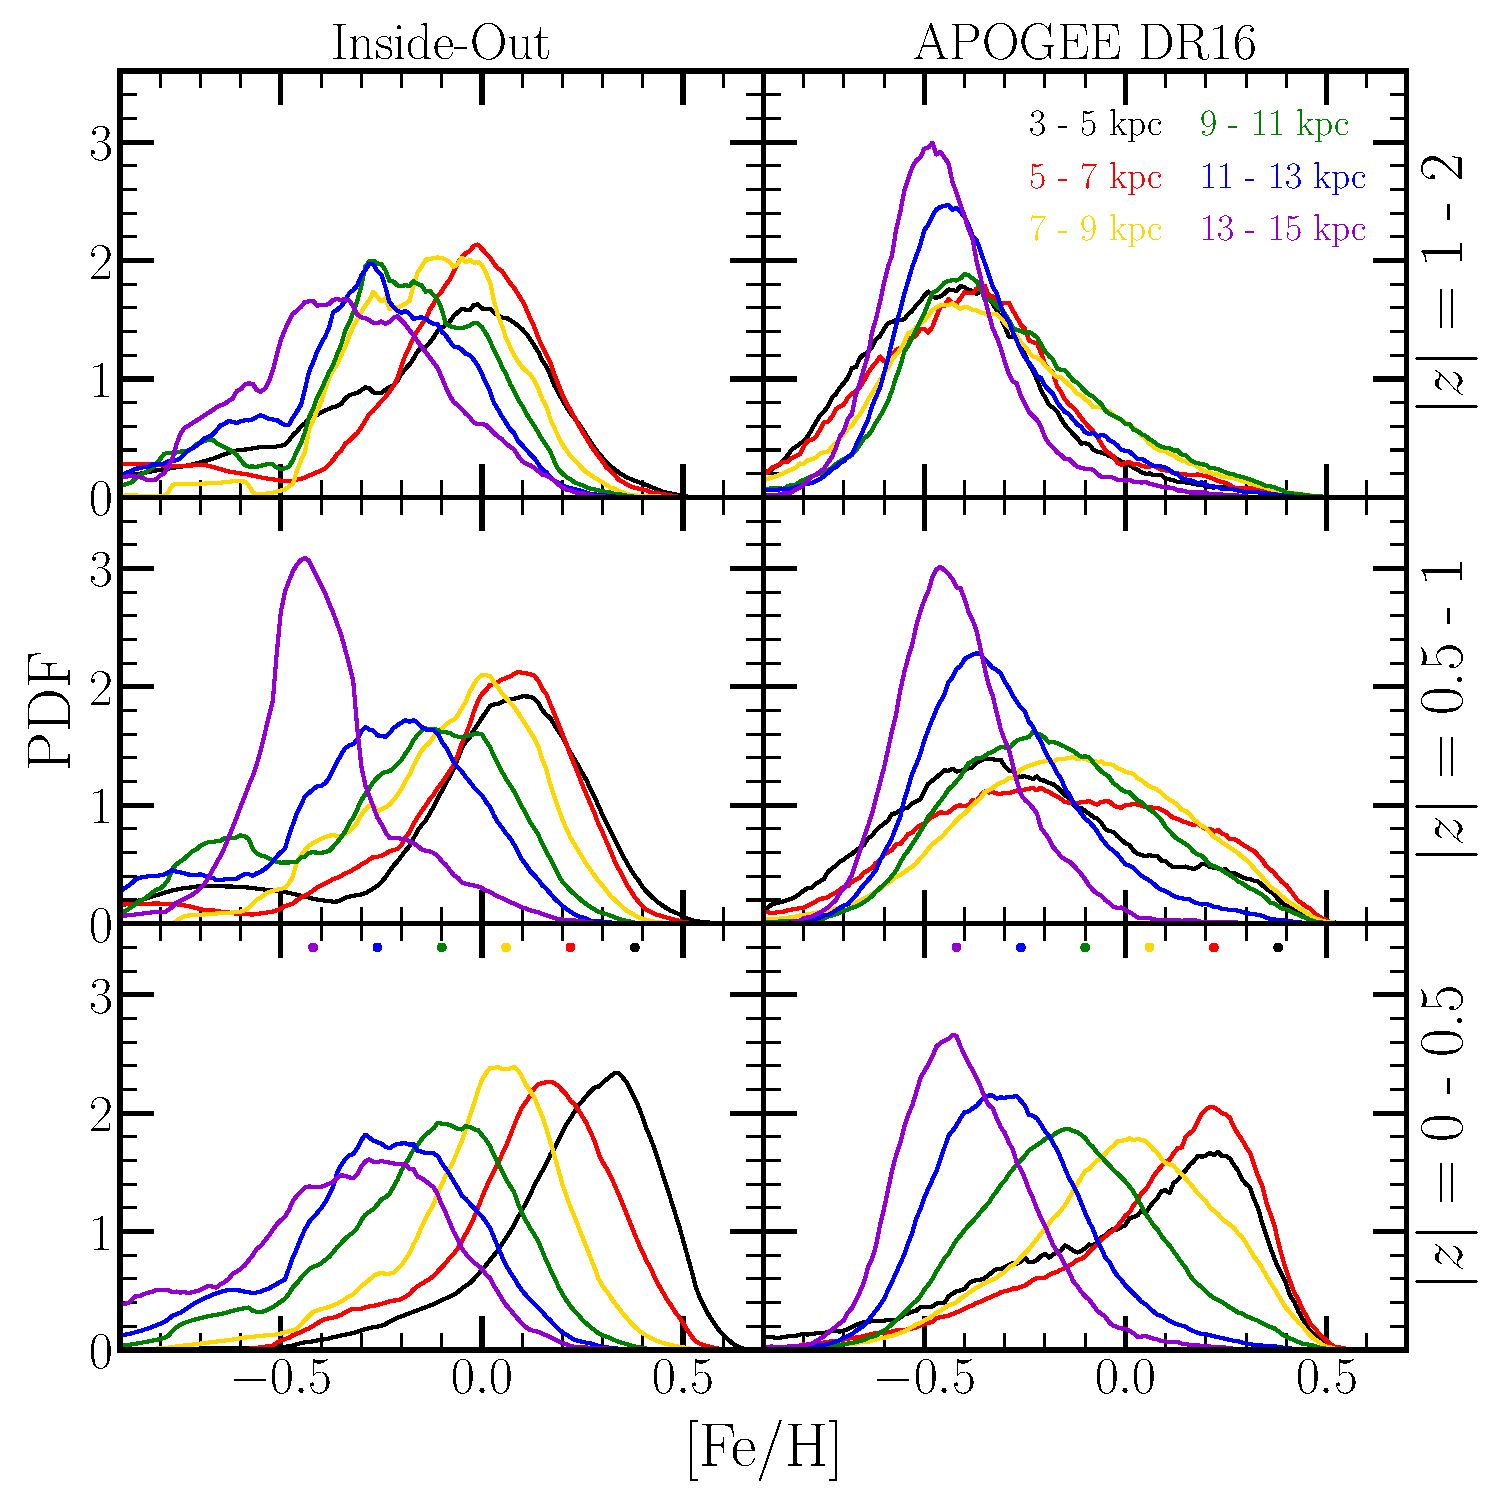
\includegraphics[scale = 0.34]{mdf_3panel_fe.pdf} 
\caption{Metallicity Distribution Functions in [Fe/H] predicted by our 
fiducial model (left) and as observed in APOGEE DR16 (right), for stars and 
simulated stellar populations with present day $\left|z\right|$ = 0 - 0.5 kpc 
(bottom), 0.5 - 1 kpc (middle), and 1 - 2 kpc (top). MDFs are shown in bins 
of Galactocentric radius: 3 - 5 kpc (black), 5 - 7 kpc (red), 7 - 9 kpc 
(yellow), 9 - 11 kpc (green), 11 - 13 kpc (blue), and 13 - 15 kpc (purple). 
The points near the top of the bottom panels denote what the mode abundance 
would be if it followed our target gradient of [Fe/H] = +0.3 at $R_\text{gal}$ 
= 4 kpc and a slope of -0.08 kpc$^{-1}$, assuming the inner radius of each bin 
(i.e. there is no point plotted for 15 kpc). All distributions are smoothed 
with a box-car width of [Fe/H]~$\pm$~0.1. } 
\label{fig:mdf_3panel_fe} 
\end{figure} 

% fig 11 
\begin{figure} 
\centering 
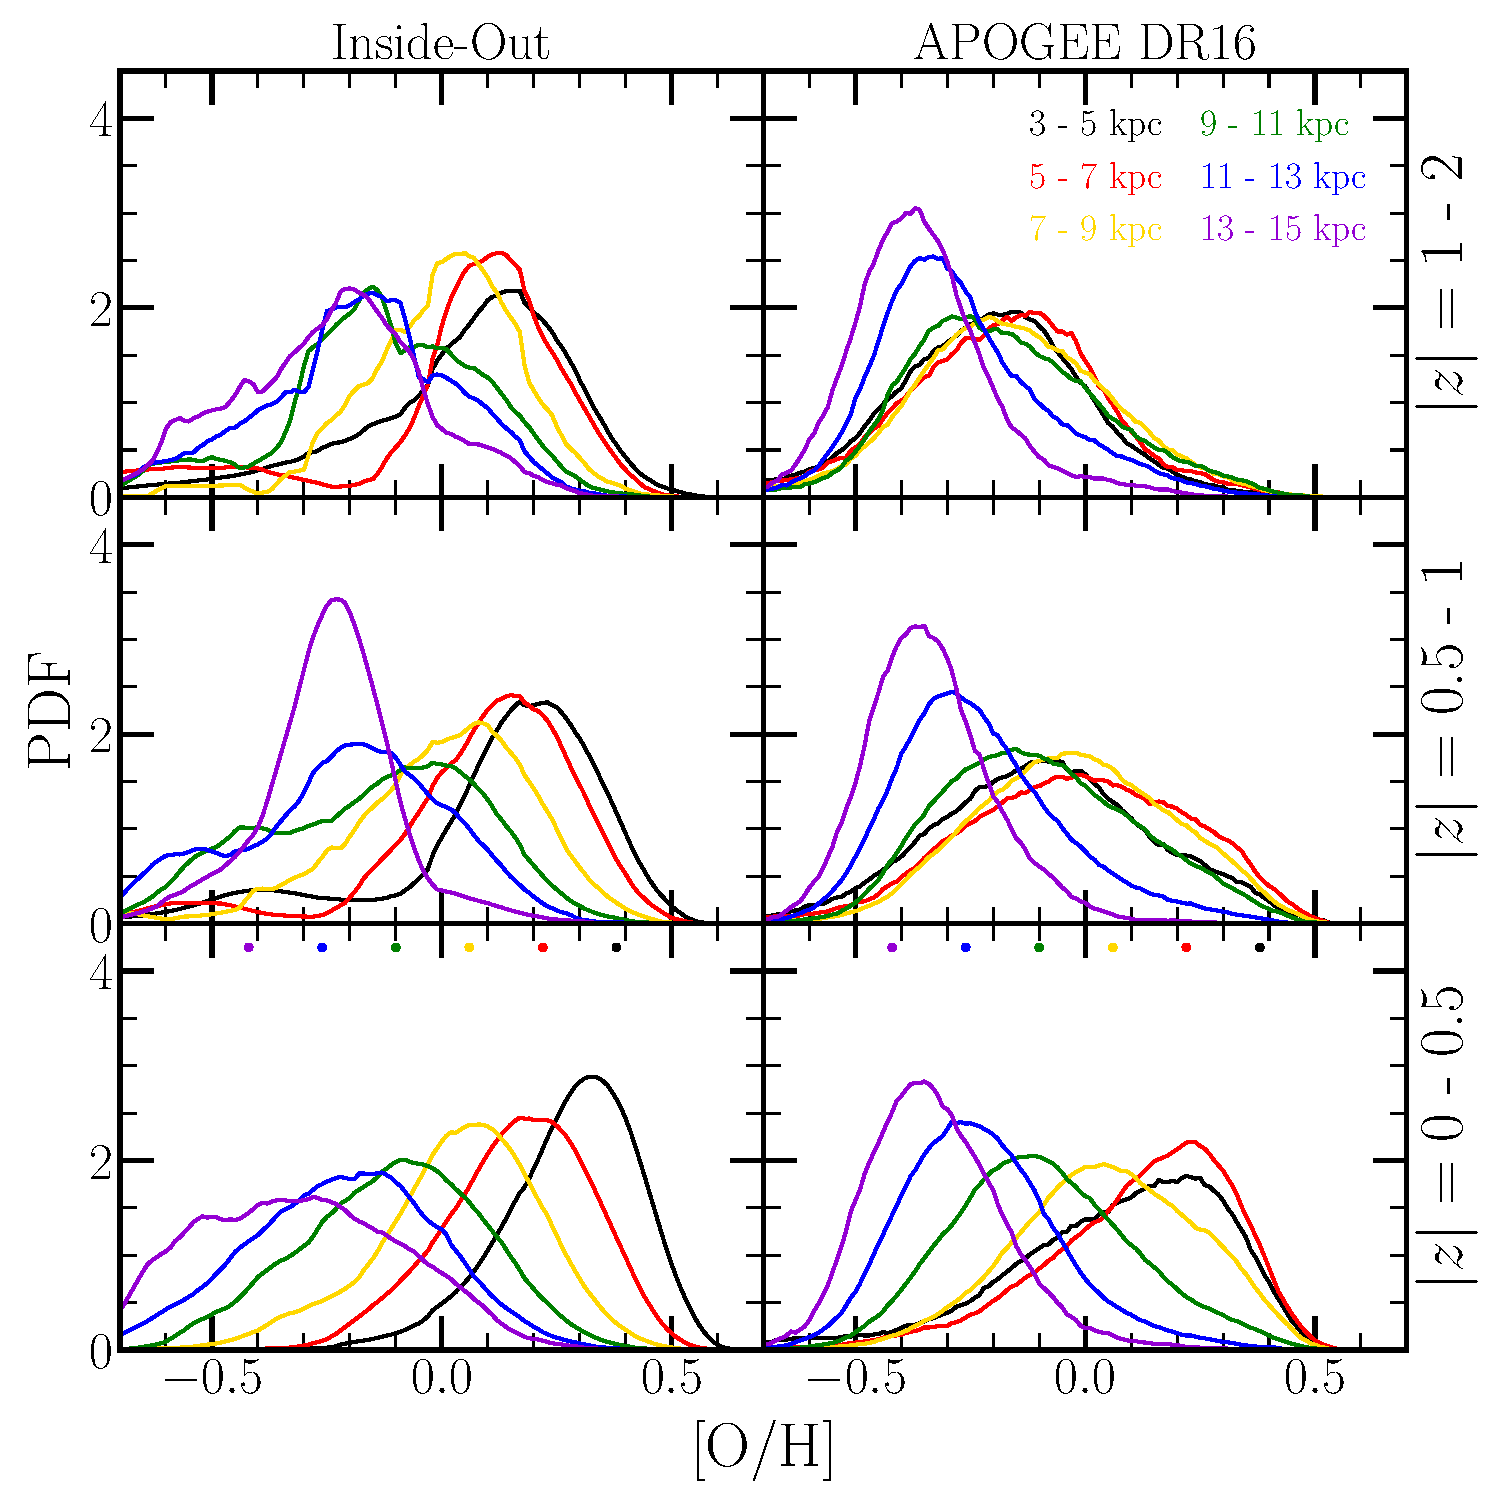
\includegraphics[scale = 0.34]{mdf_3panel_o.pdf} 
\caption{The same as Fig.~\ref{fig:mdf_3panel_fe}, but for [O/H].} 
\label{fig:mdf_3panel_o} 
\end{figure} 

% fig 12 
\begin{figure*} 
\centering 
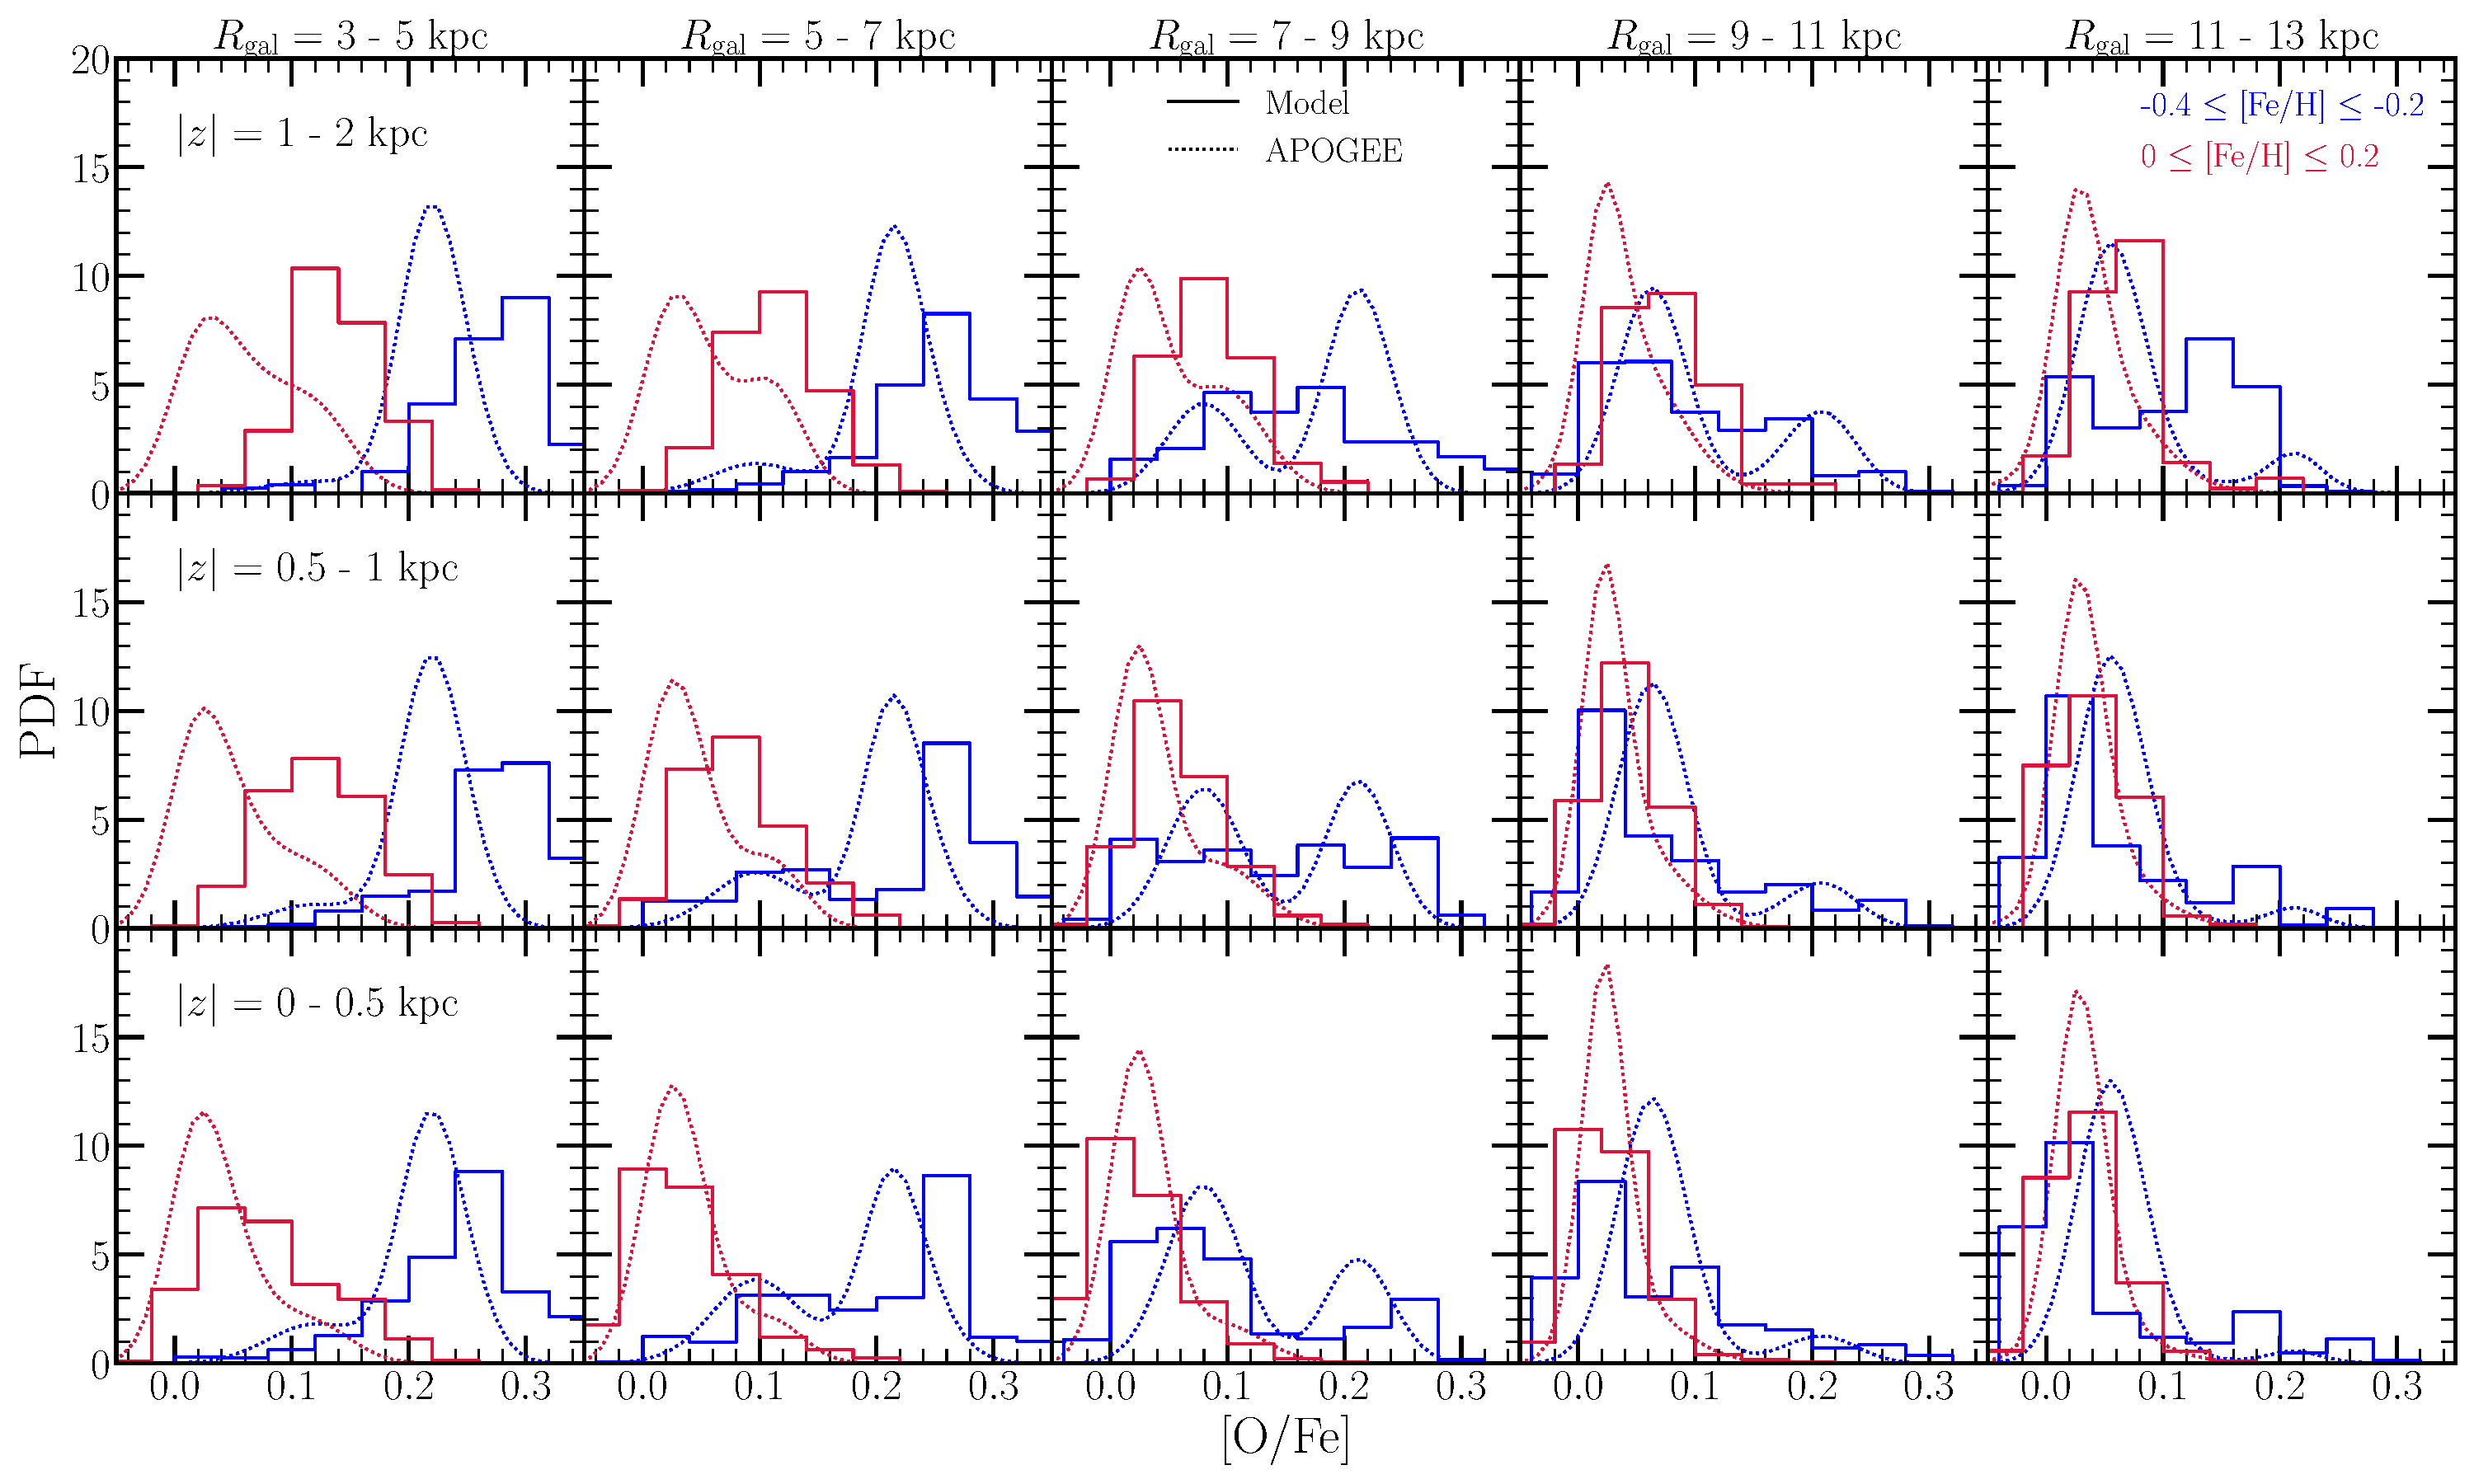
\includegraphics[scale = 0.32]{ofe_mdfs.pdf} 
\caption{Predicted distributions in [O/Fe] in 15 Galactic regions and in two 
bins in [Fe/H]. Columns correspond to bins in~$R_\text{gal}$, denoted at the 
top of each column. Rows correspond to bins in~$\left|z\right|$, denoted in 
text in the left-hand column. Distributions are color-coded according to the 
[Fe/H] the sample is drawn from, denoted by the legend in the upper right 
panel. Solid lines represent that predicted by our inside-out SFH in 
$\Delta$[O/Fe] = 0.04 bins, while dashed lines correspond the fits to the 
APOGEE DR16 data presented in \citet{Vincenzo2021}, which quantify the 
intrinsic distributions accounting for observational uncertainties and the 
APOGEE selection function. }
\label{fig:ofe_mdfs_insideout} 
\end{figure*} 

\begin{itemize} 
	\item Previously known that the MDFs in the disc midplane as observed in 
	APOGEE show mode [$\alpha$/H] and [Fe/H] abundances that depend on 
	Galactocentric radius, with a skew-negative distribution in the inner 
	Galaxy and a skew-positive distribution in the outer Galaxy. Off the 
	midplane, the MDFs merge and converge on [$\alpha$/H]~$\approx$~[Fe/H] 
	$\approx$~-0.5~\citep{Hayden2015, Weinberg2019}. This result is 
	replicated for the observations in the right-hand column of panels in Fig. 
	\ref{fig:mdf_3panel_fe} and Fig.~\ref{fig:mdf_3panel_o}. 
	\begin{itemize} 
		\item Similar mode [O/H] and [Fe/H] between the 3 - 5 and 5 - 7 kpc 
		in the APOGEE observations. What could be the origin of this? One 
		possibility is that our formalism for~$\eta(R_\text{gal})$ is 
		incorrect. We would expect a both a flat [X/H] gradient and MDFs with 
		similar modes if we simply chose it to be so by letting $\eta$ be 
		constant in the inner galaxy. Another possibility is the cessation of 
		star formation in the inner Galaxy (see Fig. 1 of~\citealp{Peek2009} 
		and Fig. 2 of~\citealp{Fraternali2012}), an effect which also isn't 
		included in our models. If the Milky Way has begun quenching, a process 
		believed to begin in the centres of galaxies at this mass 
		\citep[e.g.][]{Ellison2020b}, then few stars would form in the most 
		metal-rich regions, cutting off the MDF at high [O/H] and [Fe/H]. 
	\end{itemize} 

	\item Left-hand panels of Figs.~\ref{fig:mdf_3panel_fe} 
	and~\ref{fig:mdf_3panel_o} show the distributions predicted by our 
	late-burst model. They successfully replicate the qualitative result that 
	the mode [X/H] varies with present-day Galactocentric radius, but fail to 
	show a similar mode abundance between the 3 - 5 and 5 - 7 kpc bins. 
	Potentially linked to the cessation of star formation in inner 
	Galaxy~\citep{Peek2009, Fraternali2012}, not included in our models. 

	\item Beyond the midplane, our models fail to fully replicate the 
	convergence of the MDFs at [X/H]~$\approx$~-0.5. The observed MDF at 
	small radii shifts from skew-negative with a metal-rich mode to 
	skew-positive with a metal-poor mode with increasing $\left|z\right|$. In 
	our predicted MDFs for the inner galaxy, the mode does shift to lower 
	[X/H], though not to the same extent as in the observations. There is also 
	very little change in skewness with~$\left|z\right|$ predicted, in tension 
	with observations. 

	\item We note that our models do a good job of producing a mode [X/H] 
	abundance in each radial bin close to our target gradient (shown as 
	points plotted at the top of the bottom panels in Fig. 
	\ref{fig:mdf_3panel_fe} and~\ref{fig:mdf_3panel_o} for the inner radius of 
	each 2 kpc bin). In the inner galaxy bins, the predicted mode is 
	moderately lower than the target, but this is due to the effect of 
	dilution (see discussion in~\S~\ref{sec:comp_obs:amr}). In our inside-out 
	and outer-burst models, the difference in target and predicted mode [X/H] 
	is considerably smaller. 
\end{itemize} 

\subsection{[O/Fe] Distributions in Bins of [Fe/H]} 
\label{sec:comp_obs:mdfs:ofe} 

\begin{itemize} 
	\item In this section we compare our model predicted [O/Fe] distributions 
	to those published in~\citet{Vincenzo2021}. These are intended 
	to simultaneously remove the effects of observational errors in [O/Fe] 
	and the APOGEE selection function in these Galactic regions; that is, 
	these are estimates of the~\textit{intrinsic} [O/Fe] distributions that, 
	when convolved with observational uncertainties and the APOGEE selection 
	function, would resemble the observed MDFs. 

	\item Fig.~\ref{fig:ofe_mdfs_insideout} show distributions in [O/Fe] in 
	two bins of [Fe/H] across 15 Galactic regions predicted by our inside-out 
	SFH (solid lines). Dashed lines show the~\citet{Vincenzo2021} distributions. 

	\item We note that our model adequately reproduces the broad nature of the 
	[O/Fe] distributions at fixed [Fe/H] seen in the APOGEE data. A number of 
	distributions show a bimodality in decent agreement with the observations 
	(e.g. the -0.4~$\leq$ [Fe/H]~$\leq$ -0.2 bin at~$R_\text{gal}$ = 3 - 5 kpc 
	and~$\left|z\right|\leq$ 0.5 kpc), but this is not true of all Galactic 
	regions in both metallicity bins. Instead, the the principle failure of a 
	number of these distributions is that they overpredict the number of 
	intermediate [O/Fe] stars. While our model is successful in some ways with 
	regards to reproducing these distributions, it fails to describe the 
	observations in detail in this way. 

	\item In the inner galaxy, we overestimate the [O/Fe] of the highest 
	[Fe/H] stars at all $\left|z\right|$, and the differences in the 
	distributions gets smaller with increasing~$R_\text{gal}$. The lower 
	[Fe/H] bins don't seem to have this problem. 
	\begin{itemize} 
		\item At fixed~$R_\text{gal}$ and [Fe/H], the Vincenzo et al. (2021, 
		in prep) MDFs show two peaks in the distribution which do not change 
		with~$\left|z\right|$; only their relative heights vary. This is an 
		assumption built into the model, but the agreement with the APOGEE data 
		is good. At small~$R_\text{gal}$, the observed distributions may shift 
		slightly to higher [Mg/Fe], but only at the~$\lesssim$0.05 level 
		between~$\left|z\right|\leq$~0.5 and 1~$\leq\left|z\right|\leq$~2.0 
		(see their Fig. X). In contrast, our model predicted distributions show 
		an increase in the mode [O/Fe] of~$\sim$~0.1 over the same dynamic 
		range in~$\left|z\right|$. This suggests that our model overpredicts 
		the increase of [O/Fe] with increasing~$\left|z\right|$ compared to the 
		APOGEE distributions. 

		\item Small~$R_\text{gal}$ and high~$\left|z\right|$ is a Galactic 
		region where the APOGEE data are few, and the stellar number density is 
		high, so it's possible the observations aren't well characterized. 
		Indeed, in the~$R_\text{gal}$ = 3 - 5 and 5 - 7 kpc bins at 
		$\left|z\right|$ = 1 - 2 kpc, the~\citet{Vincenzo2021} model 
		is fit to 31 and 17 stars, respectively. In comparison, there are 109 
		in the solar annulus, and all other bins have >75 stars in the fit. 

		\item If this discrepancy persists in subsequent APOGEE data releases, 
		it's possible the origin is tied to the Sagittarius dwarf. The 
		\texttt{h277} simulation had a major merger at a lookback time of 
		$\sim$10 Gyr, and another close to the present day ({\color{red} verify 
		this, and provide citation}), different timing than the pericentric 
		passages of the Sagittarius dwarf~\citep{RuizLara2020}. More 
		pericentric passages of a massive satellite could kinematically 
		heat low-[$\alpha$/Fe] disc stars to higher~$\left|z\right|_\text{max}$ 
		orbits, shifting these distributions to lower [O/Fe]. {\color{red} This 
		is another instance where running these models with a different 
		hydro-sim's star particles could be enlightening. } 

		\item Another possibility: details of the dynamical history? Could 
		bar evolution have something to do with it? Again, a different 
		dynamical history via another hydro-sim would be enlightening. 
	\end{itemize} 

	\item Similar results are found for our other SFHs. 

	\item While the notion that an [$\alpha$/Fe] dichotomy can arise out of 
	radial migration alone was put forth in~\citet{Schoenrich2009}, and later 
	explored by~\citet{Nidever2014}, this suggests that an inside-out star 
	formation history combined with stellar migration is not conducive to 
	predicting this observed result. The principle failure of this model is 
	that it overpredicts the abundance of intermediate [$\alpha$/Fe] stars. 
	This could point to a handful of things. 
	\begin{itemize} 
		\item If the bimodality is to arise out of inside-out Galaxy evolution 
		and radial migration alone, the transition between low- and 
		high-$\alpha$ sequences needs to occur faster than it does in these 
		models. The analytic models of~\citet{Weinberg2017} suggest that the 
		approach to chemical equilibrium occurs on the order of the SFE 
		timescale~$\tau_\star$. Although we've adopted a star formation law 
		which is motivated by observational results (see discussion in~\S 
		\ref{sec:methods:sfe}), the failure of these models to reproduce the 
		observed results suggests that inside-out Galaxy growth with such a 
		star formation law is not conducive to forming the infamous 
		dichotomy. 

		\item Under our current assumptions, the simplest way to achieve this 
		is to simply shut off star formation during the intermediate 
		[$\alpha$/Fe] phase in the simulations. This is indicative that 
		two-infall evolutionary histories~\citep[e.g.][]{Chiappini1997, 
		Chiappini2001, Romano2010, Grisoni2017, Noguchi2018, Spitoni2016, 
		Spitoni2018, Spitoni2019, Spitoni2020, Spitoni2021} would improve the 
		agreement between our model predictions and the observed 
		distributions. 
	\end{itemize} 

\end{itemize} 


\subsection{The Age-[$\alpha$/Fe] Relation} 
\label{sec:comp_obs:age_alpha} 

% fig 13 
\begin{figure*} 
\centering 
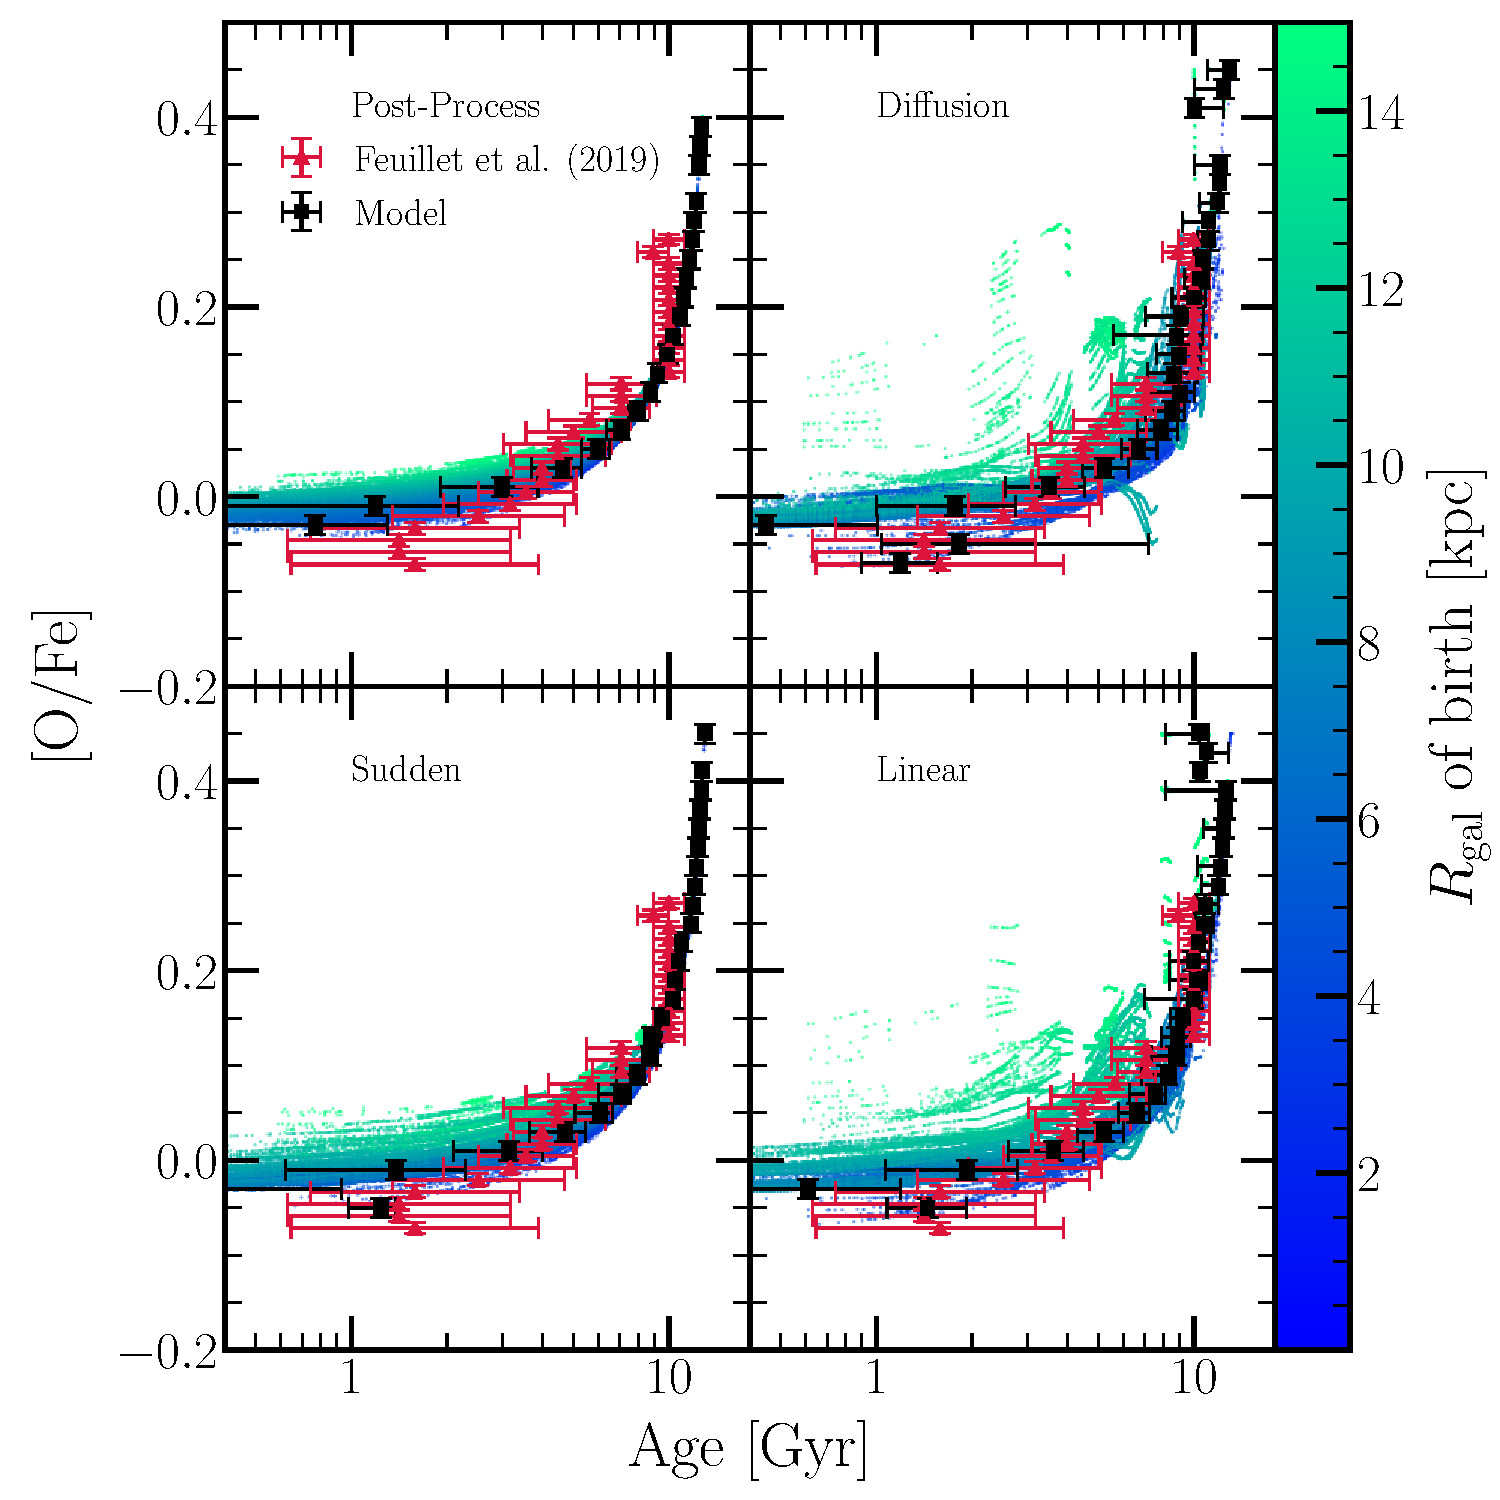
\includegraphics[scale = 0.34]{age_ofe_migration_comparison.pdf} 
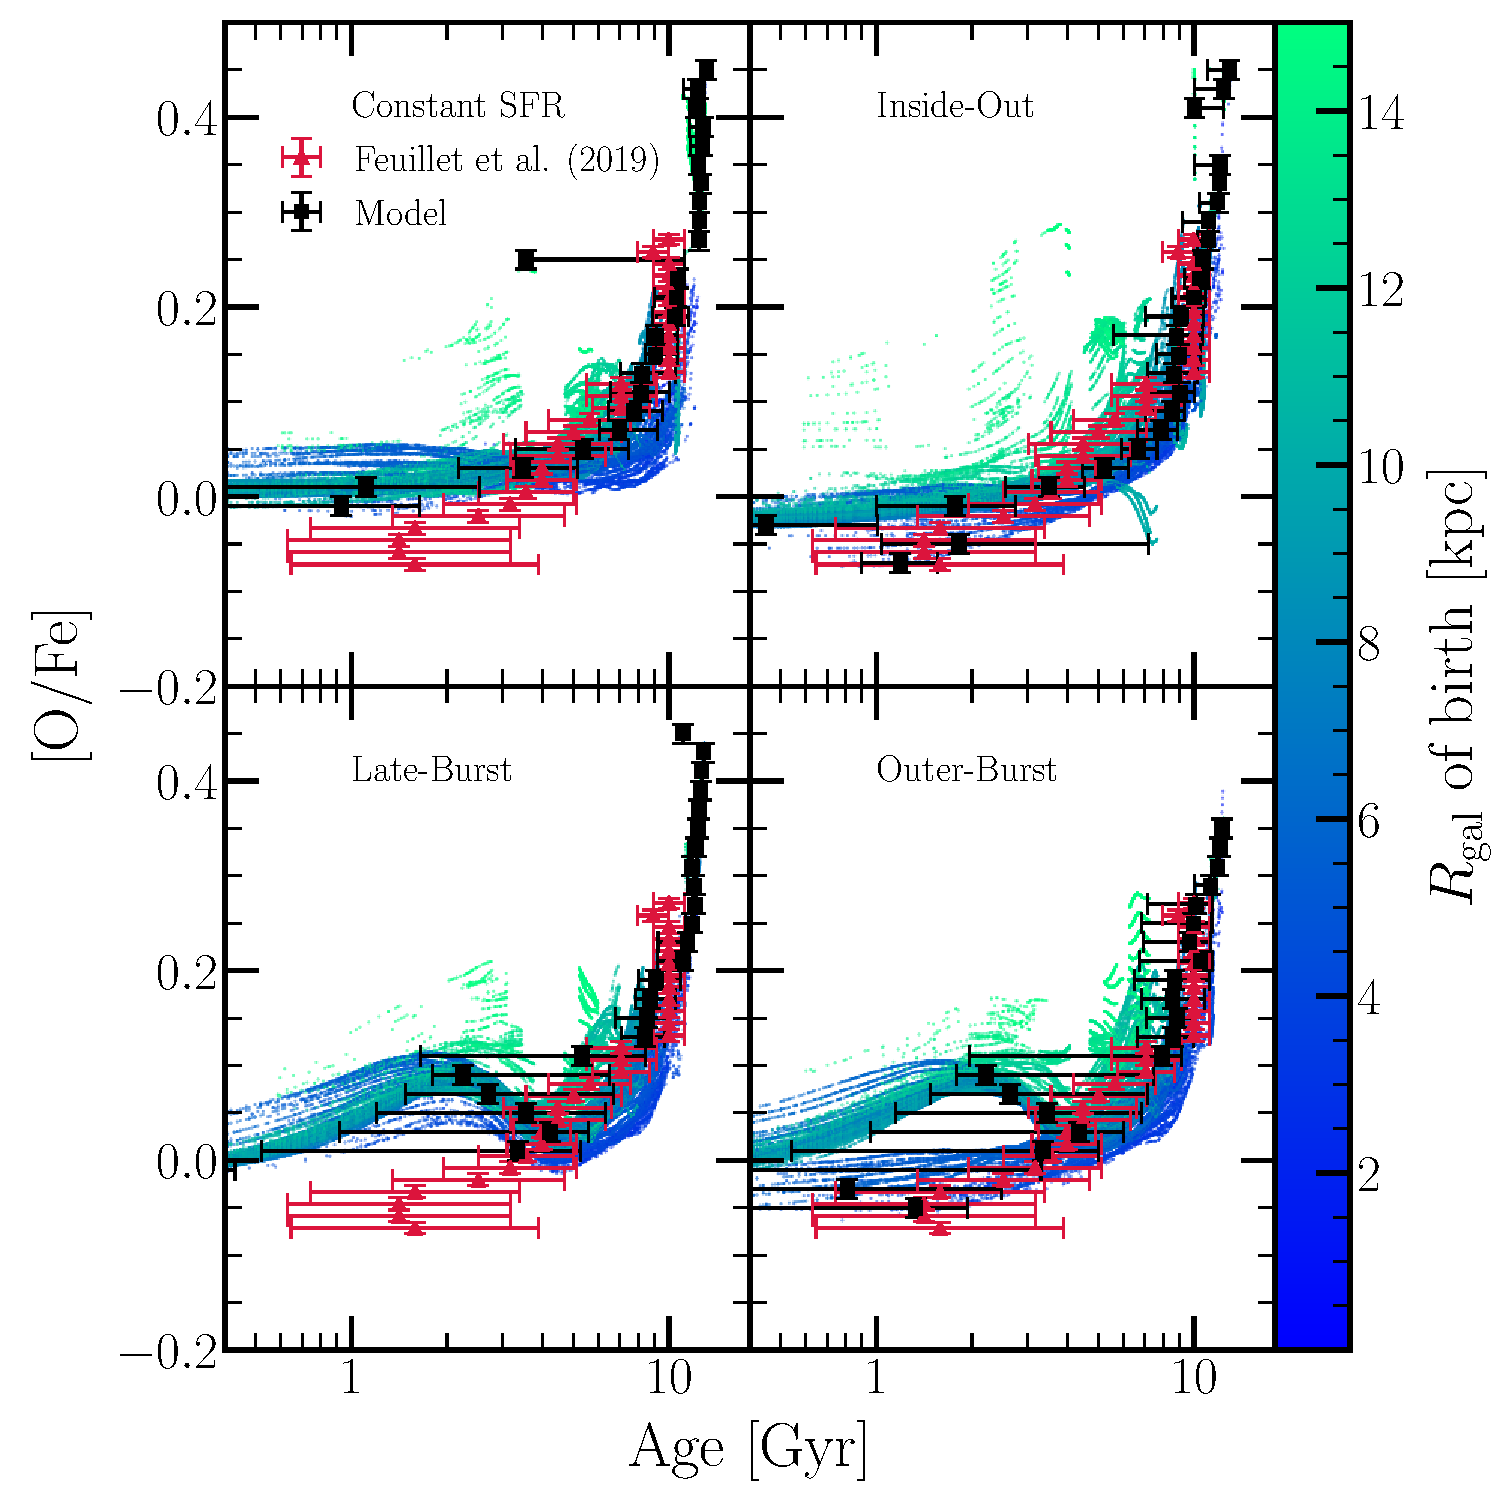
\includegraphics[scale = 0.34]{age_ofe_sfh_comparison.pdf} 
\caption{
\textbf{Left}: A comparison of the predicted age-[O/Fe] relation for the 
solar annulus ($R_\text{gal}$ = 7 - 9 kpc and $\left|z\right|\leq$ 0.5 kpc) 
between the post-processing (upper left), diffusion (upper right), sudden 
(lower left), and linear (lower right) migration models, assuming our 
inside-out SFH. 
\textbf{Right}: The same as the left-hand panels, instead comparing the impact 
of our constant (upper left), inside-out (upper right), late-burst (lower 
left), and outer-burst (lower-right) SFHs, assuming diffusion migration. 
In all panels, red triangles and error bars denote the observed mean age and 
dispersion thereof in bins of [O/Fe] as reported by~\citet{Feuillet2019}; here 
we include only the bins containing at least 15 stars. Black squares denote 
the mass-weighted median age in 0.02-dex bins in [O/Fe] predicted by the 
simulations, with error bras denoting the 16th and 84th percentiles of the 
mass-weighted age distribution in those bins. Points in the background denote 
each individual stellar population from the simulation with a final position 
in the solar annulus, color-coded according to their Galactocentric radius of 
birth. 
} 
\label{fig:age_alpha} 
\end{figure*} 

% fig 14 
\begin{figure*} 
\centering 
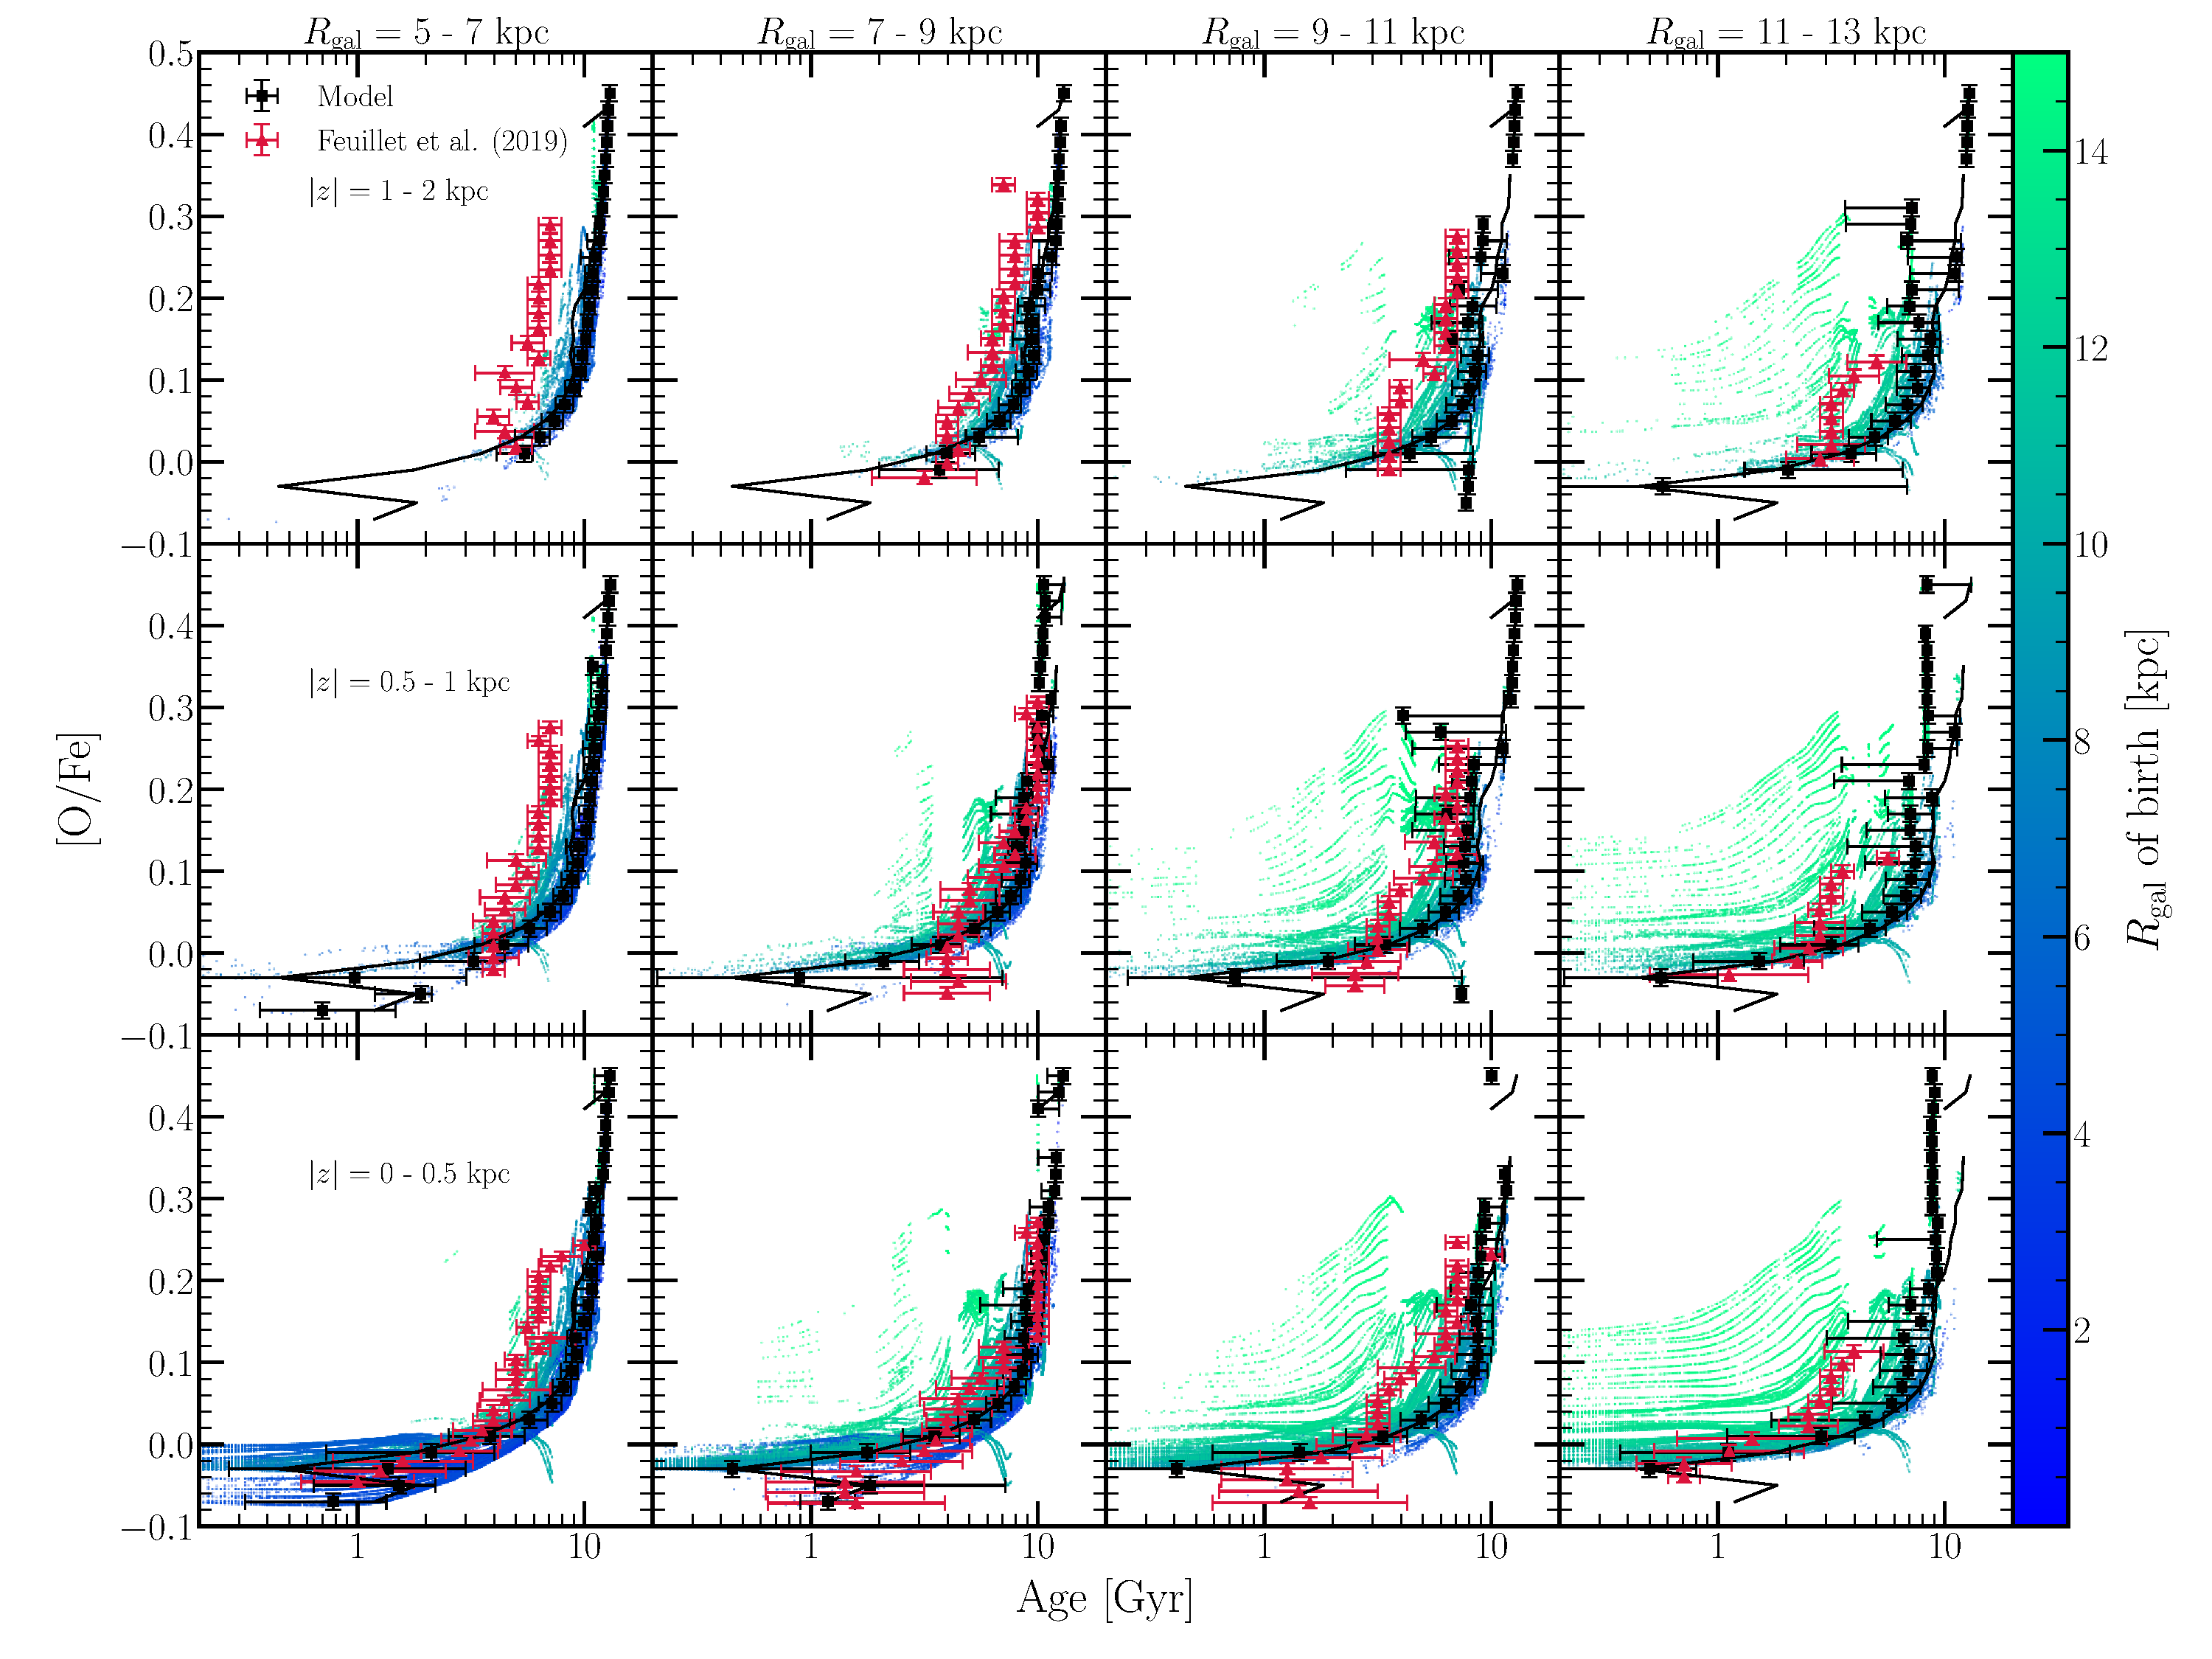
\includegraphics[scale = 0.32]{age_alpha_regions.pdf} 
\caption{The age-[O/Fe] relation in 12 galactic regions predicted by 
our inside-out SFH. Bins in Galactocentric radius are shown in columns, 
and labeled at the top. Bins in the height $\left|z\right|$ above/below the 
disc midplane are shown in rows, noted in the left-hand column. Red triangles, 
black squares, error bars, and background points are as in 
Fig.~\ref{fig:age_alpha} for the corresponding Galactic 
region. The solid black line connects the black squares in the bottom, 
left-middle panel, and is replicated in elsewhere for reference. 
} 
\label{fig:age_alpha_regions} 
\end{figure*} 

\begin{itemize} 
	\item In this section, we compare our model predictions to the 
	observational results of~\citet{Feuillet2019}. While we made use of 
	APOGEE DR16 data in comparing our model predictions to the observed 
	MDFs~\citep{Ahumada2020, Majewski2017}, they make use of DR14 stars which 
	have Gaia parallax measurements available~\citep[][for details on the 
	APOGEE survey, see discussion in~\S~\ref{sec:comp_obs:mdfs}]{Abolfathi2014, 
	GaiaDR2}. With their spatial and quality cuts, the final sample consisted 
	of 77,562 stars. 

	\item \citet{Feuillet2019} ages are measured via isochrone matching. 
	{\color{red} Potentially give a little more detail, but that may be 
	adequate for our purposes.} 

	\item In bins of [O/Fe], they assume a gaussian log-age distribution, and 
	fit the mean and standard deviation to the observed sample. Because they 
	assume a gaussian, they would report an equal mean and median. This is an 
	important caveat in comparing our predicted relations to their results, 
	because our model-predicted age distributions in bins of abundace are 
	highly non-gaussian. 

	\item The stellar populations from our simulations have different masses, 
	so the age-distributions must be weighted by mass, since that scales with 
	the number of stars that each stellar population represents. We therefore 
	adopt a mass-weighted median age in bins of abundance as the appropriate 
	comparison to the~\citet{Feuillet2019} data. Physically, in a given bin 
	[O/Fe], this is the age corresponding to the 50th percentile of the 
	mass-weighted age distribution of our simulated stellar populations. For 
	these reasons the comparison between our simulations and 
	\citet{Feuillet2019} isn't exactly one-to-one. {\color{red} Potentially 
	worth mentioning some of the systematics in calculating ages here as 
	well, as that's relevant information.} 

	\item Fig.~\ref{fig:age_alpha} shows a comparison 
	between the predicted age-[$\alpha$/Fe] relations in the solar annulus for 
	our four migration models assuming our inside-out SFH. 

	\item All models show reasonable agreement with the~\citet{Feuillet2019} 
	data; the population-averaged trend appears insensitive to the assumed 
	migration model. 

	\item Diffusion predicts the most intrinsic scatter, followed by linear, 
	then sudden, then post-processing. This is a consequence of the variations 
	in the SN Ia rates induced by time-dependent migration (see discussion in 
	\S~\ref{sec:comp_obs}). Further demonstration that under 
	certain migration models, the radial migration of nucleosynthetic yields 
	is statistically significant. This is also proof of concept that the 
	effect is significant for abundance ratios of elements where at least one 
	is produced by delayed nucleosynthetic sources. We therefore conclude that 
	the time-dependence of radial migration is a necessary ingredient to 
	chemical evolution models of galaxies where migration plays an important 
	role, such as our own Milky Way. The level of scatter also appears to 
	depend noticeably on which model for the time-dependence is adopted. 

	\item This mechanism can produce populations of Fe-poor or Fe-rich stars, 
	which can be misinterpreted as $\alpha$-enhanced or $\alpha$-deficient 
	stars. Due to young stars migrating into or out of a given annulus, the SN 
	Ia rate may be higher or lower than the expectation from a post-processing 
	migration model. If this difference in the SN Ia rate is sustained for of 
	order one depletion time, the ISM will be either Fe-poor or Fe-rich, and 
	the stars that form there will inherit that composition. The stars that 
	form out of that patch of ISM can then migrate to the solar annulus. This 
	effect is most significant at large Galactocentric radii where the 
	fractional amplitude of the variability in the SN Ia rate is largest, and 
	for that reason the young Fe-poor population predicted by our diffusion 
	model originates at large radii ($\gtrsim$ 12 kpc). 

	\item \citet{SilvaAguirre2018} demonstrated that the observed young 
	$\alpha$-rich stars in the solar annulus have kinematics similar to the 
	rest of the high-$\alpha$ population, and suggested that this may be the 
	result of stellar mergers or mass transfer events, producing a population 
	of truly old stars masquerading as young stars. In a sample of 51 of these 
	stars on the red giant branch,~\citet{Hekker2019} demonstrate that a 
	portion of these stars have carbon-to-nitrogen ratios consistent with 
	mass transfer events, but that others do not, indicating that either 
	they're truly young stars or the results of mergers on the main sequence. 
	Our model's prediction of intrinsically young, high [O/Fe] stars is 
	independent of this mass transfer scenario;~\texttt{VICE} does not include 
	any statistical treatment of mass transfer events. Ascertaining the origins 
	of this population therefore has implications for which of the migration 
	models investigated here is the most realistic. 

	\item Fig.~\ref{fig:age_alpha} shows a comparison between 
	the predicted age-[$\alpha$/Fe] relations in the solar annulus for our 
	four SFHs assuming diffusion migration. 

	\item Constant and inside-out SFHs describe the observed data the best. 
	Both late starburst models show a population-averaged increase in 
	[$\alpha$/Fe] at young ages which is not observed in the data. This 
	challenges the results of~\citet{Isern2019} and~\citet{Mor2019}, 
	suggesting that these results on the Milky Way recent SFH are not 
	consistent with chemical evolution models. If the Milky Way truly 
	experienced a recent starburst, something not included in our models had 
	to occur to prevent this global increase in [$\alpha$/Fe]. 

	\item Below [O/Fe]~$\approx$ +0.1, the~\citet{Feuillet2019} data seem to 
	follow a slightly steeper age-[$\alpha$/Fe] than our inside-out model 
	predicts. This could point to inaccuracies in the detailed form of the SFH 
	or the SN Ia DTD, our supernova yields, or observational [O/Fe] errors, all 
	of which are very plausible. 

	\item Fig.~\ref{fig:age_alpha_regions} presents a comparison of our 
	simulation data to the~\citet{Feuillet2019} observational data in 12 
	Galactic regions assuming the inside-out SFH. 

	\item In the disc, the inside-out SFH is a reasonable description of the 
	data for ages~$\lesssim$ 5 Gyr, above which the median ages are 
	overpredicted relative to~\citet{Feuillet2019}. Far from the midplane, our 
	model overpredicts the ages at nearly all abundances 
	where~\citet{Feuillet2019} have data, with the exception of the 
	$R_\text{gal}$ = 7 - 9 kpc and $\left|z\right|$ = 0.5 - 1 kpc region. 

	\item \citet{Feuillet2019} report ages for~$\alpha$-rich stars that are 
	younger at large~$R_\text{gal}$ and high~$\left|z\right|$, though in most 
	cases only by~$\sim$20\%. Our model, however, does not capture this effect. 
	To illustrate this, we connect the black squares in the panel corresponding 
	to the solar annulus with a solid black line, and reproduce this line in 
	all panels as a reference. If the observational result is correct, this is 
	an interesting result that our model doesn't reproduce in any of the 
	variants we have examined. 

	\item We note that the intrinsic scatter in the age-[$\alpha$/Fe] relation 
	predicted by the model grows with increasing~$R_\text{gal}$. Not only is 
	the scatter in the colored background points visibly larger, but the error 
	bars on the black points are as well, indicating that the age distribution 
	is getting statistically significantly wider at fixed [$\alpha$/Fe] with 
	increasing~$R_\text{gal}$. 
	\begin{itemize} 
		\item We identify two sources driving the increase in scatter at large 
		$R_\text{gal}$. The bulk of the scatter, at least at [O/Fe] 
		$\gtrsim$ +0.05, arises from the variability in SN Ia rates as 
		described in~\S~\ref{sec:comp_obs:metallicity_gradient}. There, we 
		demonstrated that the highest amplitude variability in the SN Ia rate 
		in our model Galaxy occurs in the outskirts of the disc where the 
		stellar number density is low. With higher variability in the SN Ia 
		rate comes a higher variability in the gas-phase [O/Fe] ratio, 
		resulting in an in-situ population whose age-[O/Fe] relation shows more 
		intrinsic scatter compared to that at small radii. The second source is 
		the change in normalization of the age-[O/Fe] relation expected for 
		different star formation timescales. With decreasing~$\tau_\text{sfh}$, 
		the age-[O/Fe] relation becomes shallower due to the delayed SN Ia 
		enrichment channel depositing Fe into a depleted gas reservoir 
		\citep{Weinberg2017}. This, coupled with the fact that the relation is 
		intrinsically shallow at young ages, produces noticeable scatter near 
		solar [O/Fe]. The comparison between the post-processing and diffusion 
		migration models in Fig.~\ref{fig:age_alpha} makes this fairly clear. 
	\end{itemize} 
\end{itemize} 

\subsection{The Age-Metallicity Relation} 
\label{sec:comp_obs:amr} 

% fig 15 
\begin{figure} 
\centering 
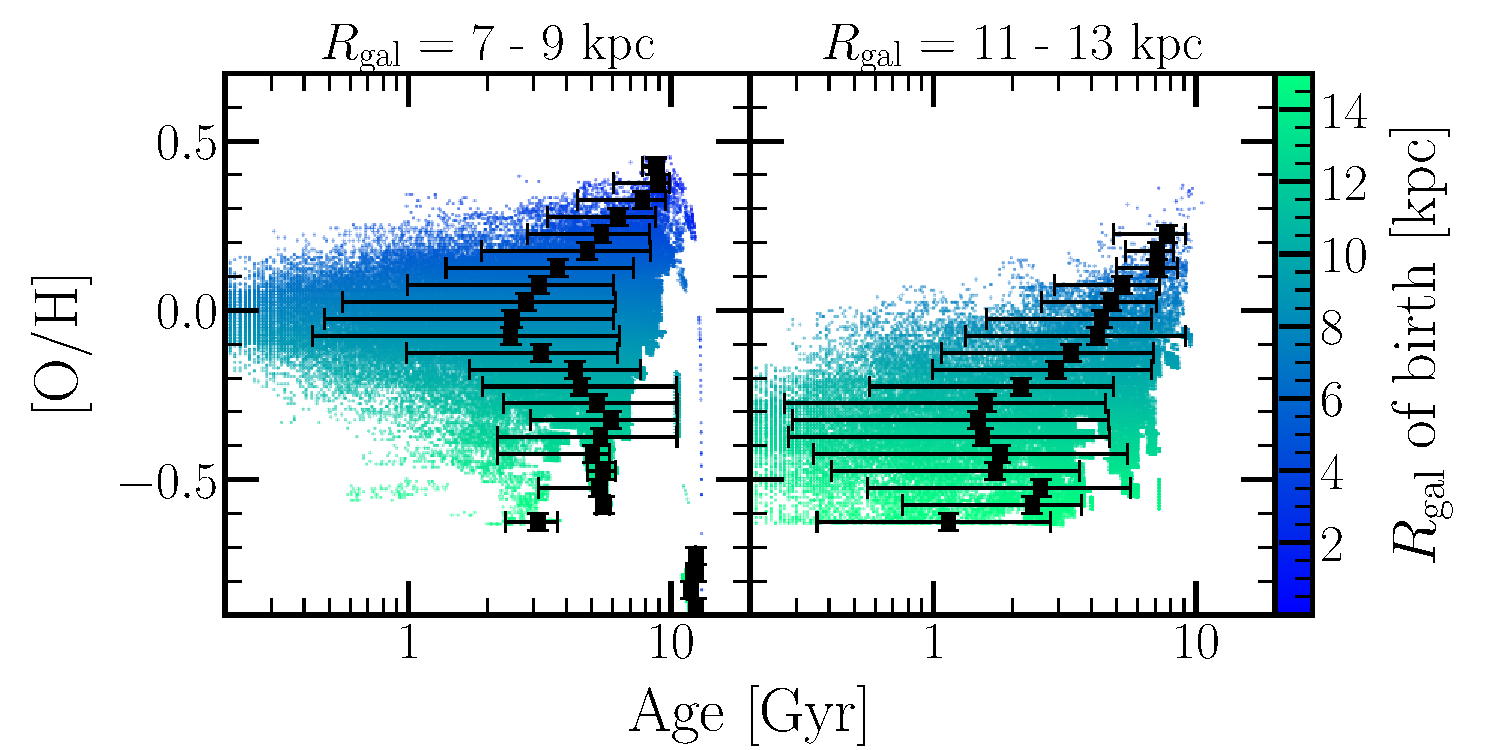
\includegraphics[scale = 0.35]{amr_static_o.pdf} 
\caption{The age-[O/H] relation predicted by our constant SFR model for 
$R_\text{gal}$ = 7 - 9 kpc (left) and 11 - 13 kpc (right). Each panel plots 
only the~$\left|z\right|\leq$0.5 kpc population. The colored points in the 
background and the black squares with error bars are as in Fig. 
\ref{fig:age_alpha}, but with our binned, simulation prediction quantified in 
0.05-dex bins in [O/H]. } 
\label{fig:age_oh_static} 
\end{figure} 

% fig 16 
\begin{figure} 
\centering 
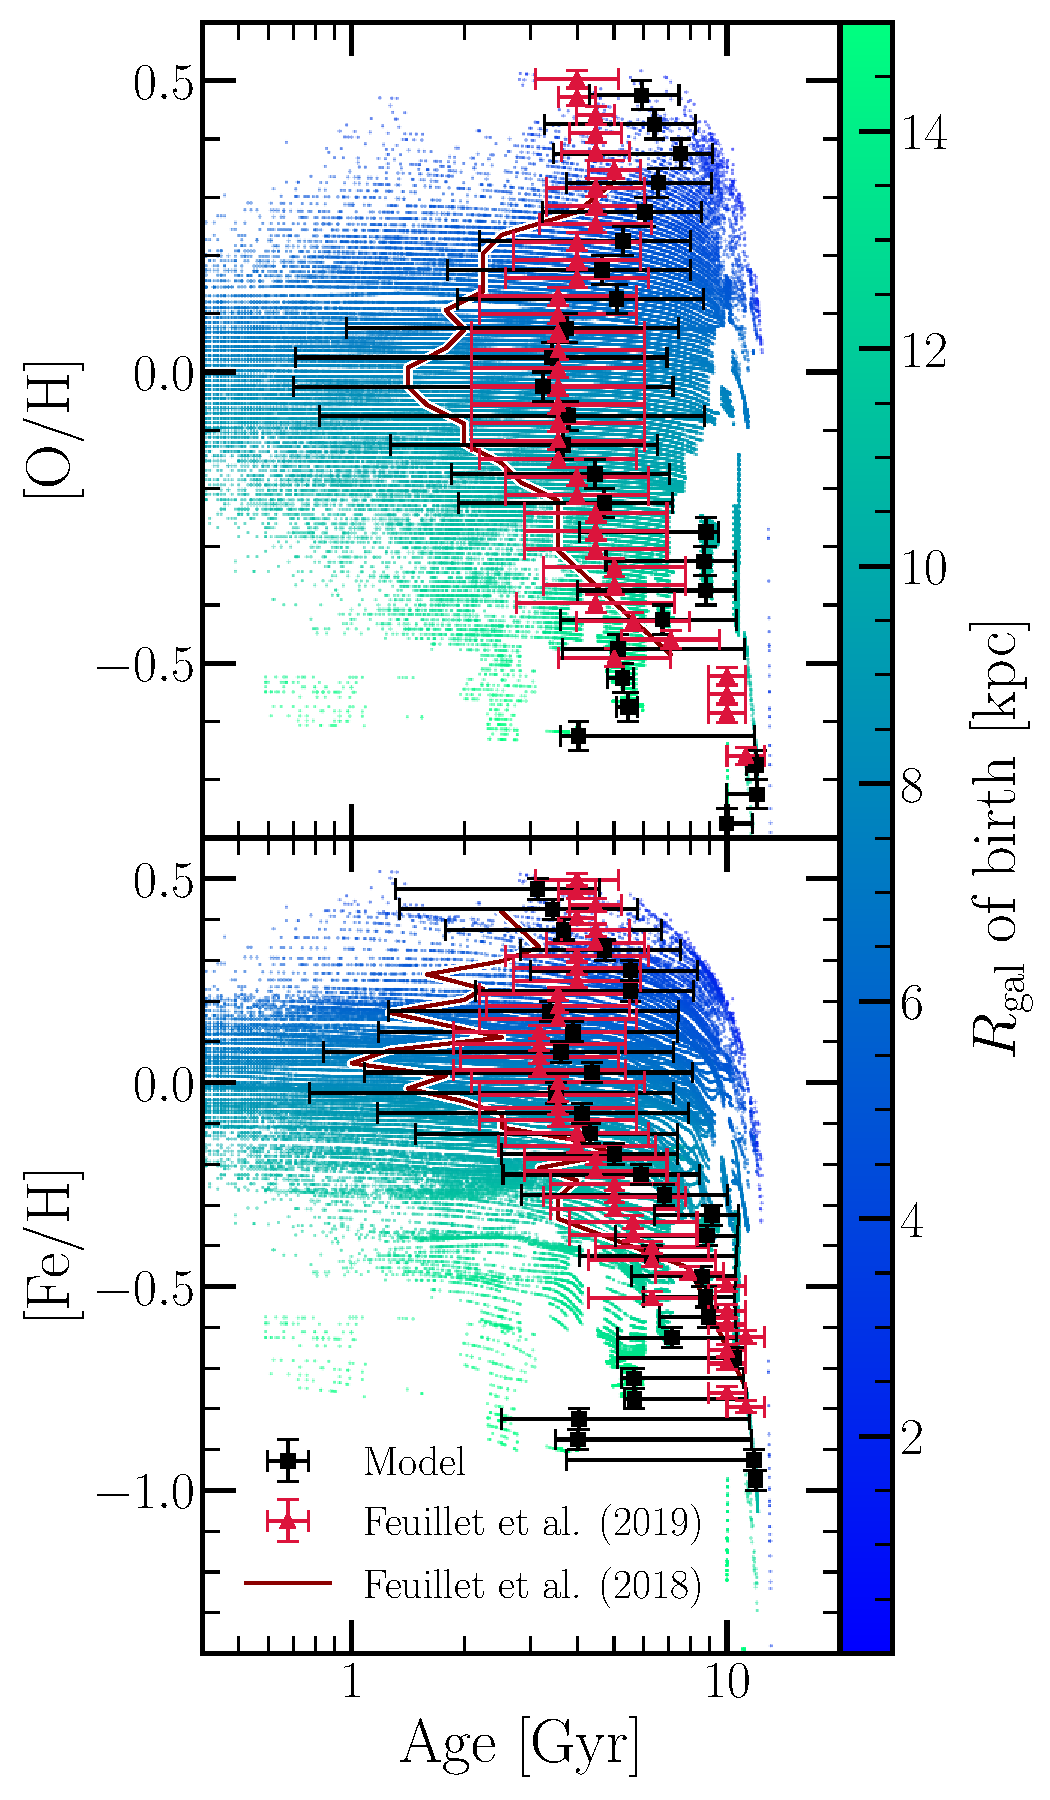
\includegraphics[scale = 0.45]{amr_solar_annulus.pdf} 
\caption{The age-[O/H] (top) and age-[Fe/H] (bottom) relations for the 
solar annulus (i.e.~$R_\text{gal}$ = 7 - 9 kpc,~$\left|z\right|\leq$ 0.5 kpc) 
as predicted by our inside-out SFH. Red triangles, black squares, error bars, 
and background points are as in Fig.~\ref{fig:age_alpha}, 
but with our simulation prediction quantified in 0.05-dex bins in [O/H] and 
[Fe/H]. For comparison, we plot the~\citet{Feuillet2018} data in a dark red 
line, omitting the associated uncertainties for the sake of clarity. } 
\label{fig:amr_solar_annulus} 
\end{figure} 

% fig 17 
\begin{figure*} 
\centering 
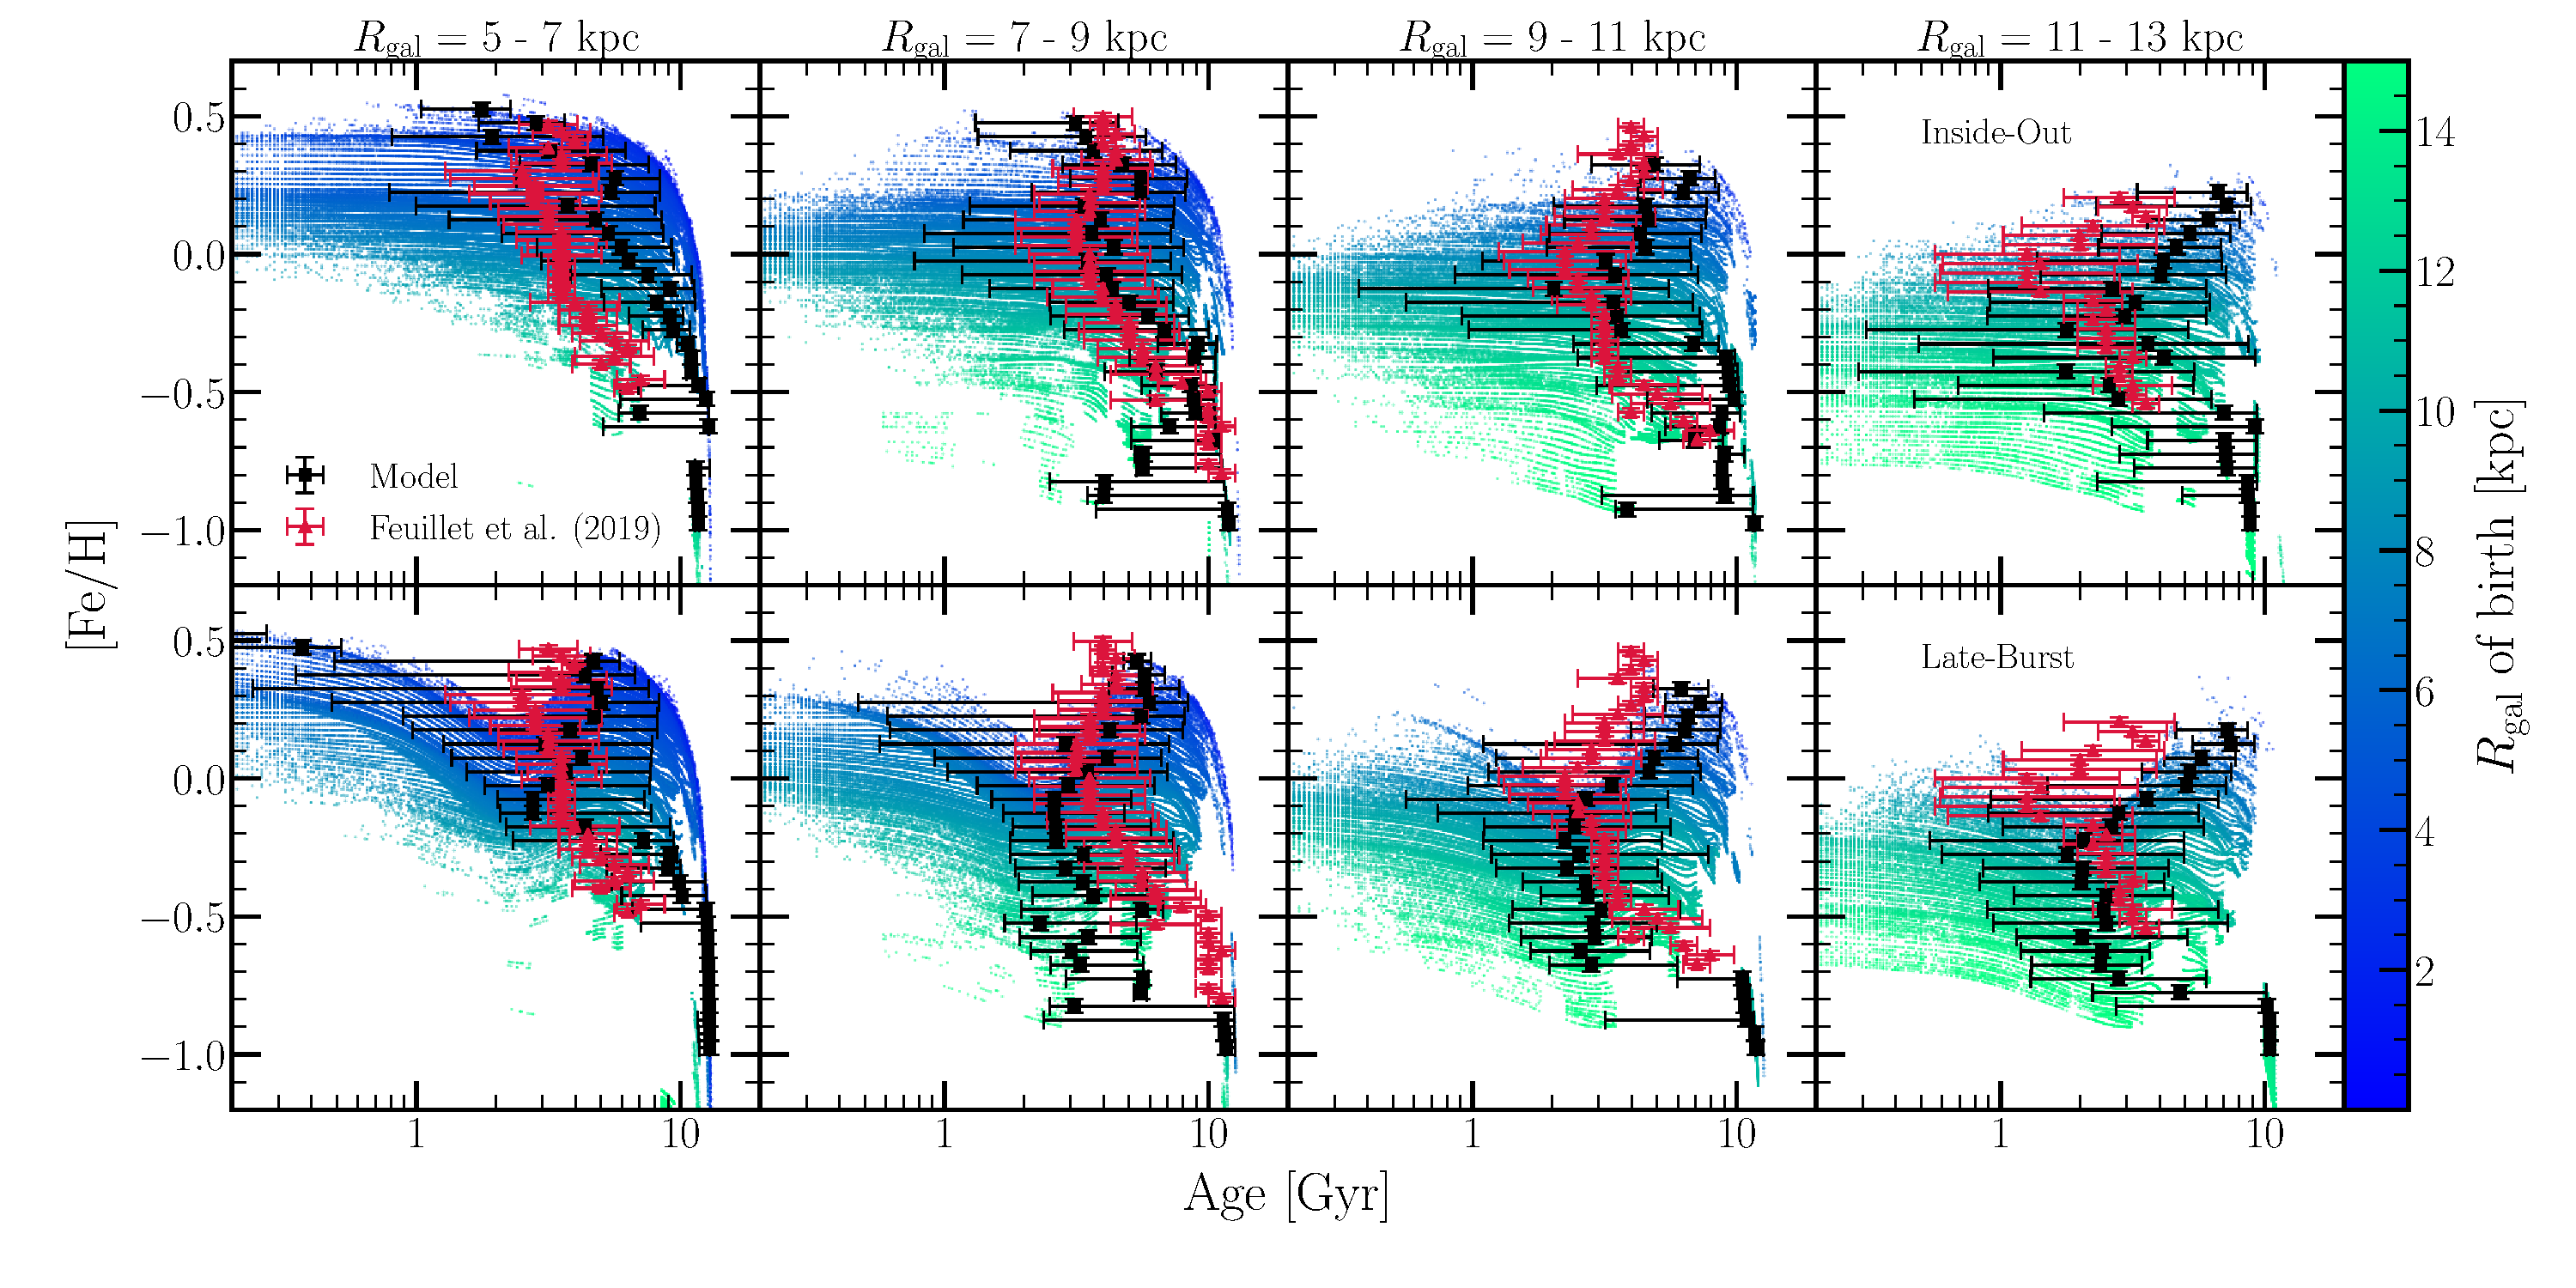
\includegraphics[scale = 0.35]{amr_insideout_vs_lateburst_fe.pdf} 
\caption{The age-[Fe/H] relation predicted by our inside-out (top) and 
late-burst (bottom) SFHs for~$R_\text{gal}$ = 5 - 7 kpc (left), 7 - 9 kpc 
(left middle), 9 - 11 kpc (right middle), and 11 - 13 kpc (right). Each panel 
plots only the~$\left|z\right|\leq$ 0.5 kpc population. Red triangles, black 
squares, error bars, and background points are as in 
Fig.~\ref{fig:age_alpha} for the corresponding 
Galactic region, but with our simulation prediction quantified in 
0.05-dex bins in [Fe/H]. } 
\label{fig:amr_insideout_vs_lateburst_fe} 
\end{figure*} 

\begin{itemize} 
	\item Although the age-metallicity relation (AMR) is usually formulated in 
	age-[Fe/H], it is also interesting to look at age-[O/H] because it is not 
	affected by SN Ia enrichment. The extent to which they differ indicates the 
	extent to which the delayed timescale and impact of migration on SN Ia 
	enrichment is important in shaping the age-[Fe/H] relation. Fig. 
	\ref{fig:age_oh_static} presents the age-[O/H] relation predicted by our 
	constant-SFH model for the~$\left|z\right|\leq$ 0.5 kpc population at 
	$R_\text{gal}$ = 5 - 7, 7 - 9, 9 - 11, and 11 - 13 kpc. The black points 
	quantify the same mass-weighted median age in bins of [O/H] as in~\S 
	\ref{sec:comp_obs:age_alpha}. Colored points in the background are also the 
	same - individual stellar populations color-coded according to birth 
	radius. We choose the constant SFH model here because it is not subject to 
	the effect of a time-varying SFH, as our fiducial inside-out SFH model is. 

	\item The intrinsic scatter in the observed AMR has been interpreted as 
	evidence for radial mixing for some time~\citep[e.g.][]{Edvardsson1993}. 
	\citet{Feuillet2018} found that most of the metal-rich stars in the solar 
	neighborhood were older than solar metallicity stars. Using the 
	\citet{Weinberg2017} analytic models of one-zone chemical evolution, they 
	argue that this is the result of old stars born at small~$R_\text{gal}$ 
	where the equilibrium abundance is high migrating to the solar 
	neighborhood. The fact that only the old stars are seen in the solar 
	annulus can then be explained by the slow nature of radial migration. 

	\item Fig.~\ref{fig:age_oh_static} extends our understanding of this 
	effect. In all regions plotted, the intrinsic scatter in the bulk 
	age-[O/H] relation increases noticeably with increasing age, and the 
	color-coding of the background points makes it clear that this arises out 
	of radial migration. At any given radius, the youngest stars form with a 
	composition reflective of the local ISM, which in our models, is in turn 
	reflective of the late-time equilibrium abundance at that radius. Stars 
	with significantly different compositions were born in different Galactic 
	regions and underwent radial migration. 
	\begin{itemize} 
		\item An interesting implication of this effect arises in the outer 
		Galaxy, visible in the~$R_\text{gal}$ = 11 - 13 kpc bin. There, the 
		equilibrium abundance is low, and the model predicts that nearly all 
		other regions of the Galaxy are forming stars at higher abundances. 
		When migration is taken into account, the result is an AMR which is 
		nearly monotonically~\textit{increasing} with age, entirely the 
		opposite of what is predicted by one-zone models. 
	\end{itemize} 

	\item Furthermore, the characteristic metallicity of the youngest stars 
	in a given radial bin decreases with increasing radius. This is a natural 
	consequence of the abundance gradient that we've built in at late times, 
	but interestingly, the effect is strong enough that at large radii, the 
	median trend is nearly monotonically increasing with age. This is 
	completely backwards from what is expected from one-zone models of 
	chemical evolution for any radius. Since this is our constant-SFR model, 
	it is not subject to the effects of a time-varying SFH, quantifying only 
	what is caused by radial migration. 

	\item Similar things are found for Fe, but the variations in the black 
	squares a bit bigger so we demonstrate the effect with [O/H]. 

	\item Fig.~\ref{fig:amr_solar_annulus} shows the age-[O/H] (top panel) 
	and the age-[Fe/H] (bottom panel) relations predicted by our fiducial 
	inside-out SFH in the solar annulus ($R_\text{gal}$ = 7 - 9 kpc and 
	$\left|z\right|\leq$~0.5 kpc), under the same plotting convention as in 
	\S~\ref{sec:comp_obs:age_alpha}. We add a solid black line to denote the 
	\citet{Feuillet2018} AMR in comparison to that of~\citet{Feuillet2019}. 
	\begin{itemize} 
		\item We note that we find similar results with regard to the 
		age-[O/H] relation predicted by our models. 

		\item \citet{Feuillet2018} shows a significantly younger median age at 
		solar metallicity in both O and Fe ($\sim$1 - 2 Gyr as opposed to 
		$\sim$2 - 3 Gyr). 

		\item Fiducial, inside-out SFH performs decently at explaining the 
		\citet{Feuillet2019} AMR, but the ages at solar metallicity in the 
		\citet{Feuillet2018} study are too young for this model. Comparing the 
		black points in this figure to those in Fig.~\ref{fig:age_oh_static} 
		suggests that the constant SFR model can't explain ages that young 
		either. If we were to take the~\citet{Feuillet2018} results at face 
		value in comparison to these models, this would strongly suggest a 
		recent enhancement at least in the local star formation rate of the 
		solar annulus to increase the frequency of~$\sim$1 Gyr old, solar 
		metallicity stars close to the sun. 

		\item Such a burst is indeed supported by the findings of 
		\citet{Mor2019}, who find a factor of~$\sim$2 enhancement in the SFH 
		of the Milky Way~$\sim$2 Gyr ago by comparing population synthesis 
		models to observed stellar luminosity functions and color-magnitude 
		diagrams with Gaia data~\citep{GaiaDR2}.~\citet{Isern2019} reach 
		similar conclusions modeling white dwarf luminosity functions in the 
		solar neighborhood with Gaia parallaxes. 
	\end{itemize} 

	\item Fig.~\ref{fig:amr_insideout_vs_lateburst_fe} shows a comparison of 
	the predicted age-[Fe/H] relation for~$\left|z\right|\leq$~0.5 kpc stars 
	in the~$R_\text{gal}$ = 5 - 7, 7 - 9, 9 - 11, and 11 - 13 kpc annuli. 
	Points are plotted in the same manner as in Fig.~\ref{fig:age_oh_static} 
	and Fig.~\ref{fig:amr_solar_annulus} in this section. 
	\begin{itemize} 
		\item Beyond the solar annuulus, we note that our inside-out SFH 
		model in general overpredicts the characteristic ages of stars 
		compared to~\citet{Feuillet2019} except for [Fe/H]~$\approx$~+0.4 and 
		-0.5. We also remark that in the trend is not very well reproduced 
		either, particularly in the~$R_\text{gal}$ = 5 - 7 kpc bin. 

		\item In the bottom row of panels, we show the same relation for our 
		late-burst SFH. Interestingly, the late-burst model improves upon the 
		failures of the inside-out model significantly. In particular, the 
		over-prediction of ages of solar and intermediate metallicity stars is 
		fixed by the late-burst model. 
		\begin{itemize} 
			\item In our recent starburst models,~\texttt{VICE} calculates 
			that there is a significant amount of low metallicity gas infall 
			required to sustain such an increase in star formation under our 
			adopted~$\dot{\Sigma}_\star-\Sigma_\text{g}$ relation (see 
			bottom two panels of Fig.~\ref{fig:evol} and~\S~
			\ref{sec:methods:sfe}). 

			\item Denoting the ages and compositions of the individual stellar 
			populations from our simulations, the colored points in the 
			background of these panels trace the metallicity of the gas as a 
			function of time at various radii. That is, the blue points also 
			represent the [Fe/H] of the gas phase at small radii at various 
			lookback times, and the same for the green points and large radii. 

			\item This demonstrates that at a lookback time of~$\sim$2 Gyr, by 
			construction, the ISM at nearly all Galactocentric radii decreased 
			in metallicity. At the same time, the star formation rates 
			increased by a factor of~$\sim$2, again by construction (see the 
			right-hand panels of Fig.~\ref{fig:evol}). The result is that at 
			any radius, the frequency of~$-0.5~\lesssim$~[O/H]~$\lesssim~0$ 
			stars at ages of~$\sim$2 Gyr is increases by a factor of~$\sim$2 
			from the inside-out model, decreasing the characteristic ages of 
			stars at these metallicities. 

			\item Although there appears to be an offset between the 
			\citet{Feuillet2019} data and our predicted AMR at high 
			$R_\text{gal}$, the late-burst model describes the observed trend 
			noticeably better than the inside-out model. Although the ages of 
			modestly sub-solar metallicity stars in the solar annulus are 
			slightly under-predicted by the model, the same can be said about 
			the trend here and at 5 - 7 kpc as well. 

			\item The parameters which control this offset are the yields of 
			Fe and the mass-loading factor as a function of~$R_\text{gal}$. 
			If we were to take a slightly higher yield of Fe, it would however 
			increase the overall normalization at~$R_\text{gal}$~< 9 kpc as 
			well, where we do not see this discrepancy. It's possible that the 
			mass-loading factor~$\eta$ (see discussion in~\S 
			\ref{sec:methods:yields}) increases too quickly at large 
			$R_\text{gal}$ in our models, or that outflows are more efficient 
			at removing individual elements from the star forming reservoir. 
			Variable metal-loading factors~$\eta_Z$ would be supported by the 
			observations of~\citet*{Chisholm2018}. 

			\item We remark that the late-burst model predicts extremely young 
			characteristic ages for the highest [Fe/H] bins in the 5 - 7 kpc 
			annulus. This is merely a consequence of the re-enrichment that 
			accompanies the ensuing starburst; in infall-driven starbursts 
			such as this, the abundances often reach super-equilibrium values 
			while the star formation rate is still perturbed, which then decay 
			together back to their pre-burst, equilibrium values 
			\citep{Johnson2020}. On 
			Fig.~\ref{fig:amr_insideout_vs_lateburst_fe}, this is noticeable 
			by the abundances on the left-hand edge of each panel being 
			higher in the late-burst scenario. The points that we have 
			plotted as characteristic ages represent that 50th percentile of 
			the mass-weighted age distribution of our stellar populations in 
			a bin of abundance; in other words, a mass-weighted 
			\textit{median}. The age-distribution at these abundances is 
			bimodal, noticeable by the colored points in the background, 
			indicating that the median may not be the best statistic for these 
			few stellar populations. We note that the outer-burst model, in 
			which $R_\text{gal}$~< 6kpc do not experience the starburst, does 
			not suffer from this issue. The minutia of the AMR at different 
			radii in our late starburst models is sensitive to the detailed 
			time-dependence of the straburst in each annulus. 
		\end{itemize} 
	\end{itemize} 

	\item Conclude that the AMR reported by~\citet{Feuillet2019} is better 
	described by our late starburst models than the inside-out model. This is 
	at odds with our findings in the same simulations with the same 
	observational dataset with regard to the age-[$\alpha$/Fe] relation. 
	Perhaps the differences can be reconciled. 
	\begin{itemize} 
		\item The models would be able to have their cake and eat it too if 
		there is a recent starburst with no ensuing $\alpha$-enhancement. This 
		is difficult to rationalize, however, because an increase in 
		[$\alpha$/Fe] in the wake of a starburst is a direct consequence of 
		the perturbed ratio of CCSN-SN Ia rates caused by the burst 
		\citep{Johnson2020}. We argue based on this that it is unlikely that 
		the detailed timing of a recent starburst would mitigate this issue. 

		\item It's possible that the Milky Way experienced dilution with no 
		ensuing starburst. This could be the case if the accreted gas was 
		mostly in the form of HI or HII that has not yet cooled and been 
		available for star formation, but has been mixing with the 
		nucleosynthetic products of ongoing star formation in the Galaxy. With 
		dilution playing a noticeable role in the AMR predicted by our burst 
		models, it's possible a model of this nature could agree with both 
		the AMR and the age-[$\alpha$/Fe] relation. This would require 
		future studies which include a treatment of a multi-phase ISM. This 
		would however be at odds with the findings of~\citet{Mor2019} and 
		\citet{Isern2019}. 
	\end{itemize} 

	\item As a general result here, we caution future studies against 
	leveraging the agreement between a chemical evolution model and 
	observational data based on the solar annulus alone. Fig. 
	\ref{fig:amr_solar_annulus} presents the comparison of our fiducial, 
	inside-out SFH model predictions in the solar annulus to the 
	\citet{Feuillet2019} data, and Fig.~\ref{fig:amr_insideout_vs_lateburst_fe} 
	compares the inside-out and late-burst predictions in a larger range of 
	radii. Had we only considered the solar annulus, we would have concluded 
	that the fiducial, inside-out model agrees with the~\citet{Feuillet2019} 
	data well. However, in considering other regions of the Galaxy, we found 
	that the inside-out model actually had a handful of failures which were 
	mitigated by our late-burst model. 

	\item With our age-[O/H] and age-[Fe/H] relations, we find similar results 
	as in~\S~\ref{sec:comp_obs:age_alpha} whereby our model 
	in general overpredicts the observed ages of stars at high 
	$\left|z\right|$. Discussion of potential sources of this can be found 
	in~\S~\ref{sec:comp_obs:age_alpha}. 
\end{itemize} 

\section{Conclusions} 
\label{sec:conclusions} 
\begin{itemize} 
	\item We have modeled the Milky Way as a series of concentric annuli with 
	$\Delta R_\text{gal}$ = 100 pc width, describing each annulus as a 
	conventional one-zone model of chemical evolution, and allowing the 
	exchange of stellar populations between zones to model the impact of 
	stellar migration on enrichment in the Galaxy. Though there have been a 
	number of studies to date with a similar treatment of the Galaxy 
	\citep[e.g.][]{Matteucci1989, Schoenrich2009, Nidever2014, Sharma2020}, 
	ours and the~\citet{Minchev2013, Minchev2014, Minchev2017} model are the 
	only which make use of hydrodynamical simulation to describe radial mixing, 
	for which we take the~\texttt{h277} zoom-in simulation. This yields a model 
	for migration which does not have any free parameters (see discussion in 
	\S~\ref{sec:methods:h277}). 

	\item Our model assumes nucleosynthetic yields and a SN Ia DTD based on a 
	combination of theoretical and empirical constrants. The main free 
	parameters are the star formation law ($\tau_\star(R_\text{gal}, T)$, see 
	\S~\ref{sec:methods:sfe}), the mass-loading factor~$\eta(R_\text{gal})$ 
	(assumed to be time-independent, see~\S~\ref{sec:methods:yields}), and the 
	SFH. The first we choose from the observed 
	$\dot{\Sigma}_\star-\Sigma_\text{g}$ relation in local spirals. The second 
	is chosen to match the metallicity gradient. The fiducial model then has an 
	inside-out SFH calibrated to the~\citet{Sanchez2020} data. We also consider 
	models with a late starburst, motivated by~\citet{Mor2019} and 
	\citet{Isern2019}, and a constant-SFH model with a theoretical motivation. 

	\item Our model predicts masses and abundances for simple stellar 
	populations, a given number of which form in a given annulus and timestep. 
	From the hydrodynamical simulation, each stellar population finds a star 
	particle from~\texttt{h277} to act as its~\textit{analog}, assigned such 
	that it the star particle was born at a similar Galactocentric radius and 
	time. The stellar population in our chemical evolution model then assumes 
	the change in radius~$\Delta R_\text{gal}$ and final height above/below the 
	disc midplane~$\left|z\right|$ of its analog at face value. 

	\item We demonstrate that the dependence of the number of high- and 
	low-$\alpha$ sequence stars on Galactic region is at least in part a 
	natural consequence of radial migration. In our models, low [Fe/H], high 
	[$\alpha$/Fe] stars are located at low~$R_\text{gal}$ and high 
	$\left|z\right|$; conversely, the high [Fe/H], low [$\alpha$/Fe] stars are 
	preferentially found at high~$R_\text{gal}$ and low~$\left|z\right|$. We 
	clarify that this is not an explanation for the~\textit{origin} of the 
	two sequences - only the positional dependence thereof. 

	\item We find that migration-induced fluctuations in the SN Ia rate are a 
	significant effect. The characteristic delay time of a SN Ia rate is of 
	order 1 Gyr~\citep{Maoz2012, Maoz2017}, while stars are migrating a 
	significant distance in the radial direction on similar timescales in our 
	models. The result is a SN Ia rate which, at fixed radius, tends to follow 
	what is expected in a one-zone model with the same SFH, but shows 
	significant variability on~$\sim$Gyr timescales. Our model also predicts 
	this variability to grow with increasing radius due to sampling noise 
	having a greater impact where the stellar number density is low. 
	\begin{itemize} 
		\item We demonstrate that this is a mechanism with which truly young, 
		high [$\alpha$/Fe] stars can be formed. In a region of time and space 
		where the SN Ia rate is lower than expected from the SFH, the ISM will 
		become Fe-poor, increasing the gas-phase [$\alpha$/Fe] ratio on 
		timescales comparable to the local gas depletion time. Stars 
		then form in this region of the ISM, encoding this composition in their 
		atmospheres, and then migrate to the solar annulus, where they're seen 
		in observations as young, super-solar [$\alpha$/Fe] stars. While 
		there's an observational argument that at least some fraction of these 
		stars are mass transfer events~\citep[e.g.][]{SilvaAguirre2018, 
		Hekker2019}, our model suggests that some fraction of the remaining 
		stars are truly young, not~$\alpha$-enhanced but Fe-poor stars. 

		\item In general, our results are broadly consistent with 
		\citet{Kubryk2013} and~\citet{Khoperskov2021}, who argue that radial 
		migration has a negligible impact on the [$\alpha$/Fe]-[Fe/H] 
		distribution over time. While we find significant deviations in the 
		gas-phase tracks between the post-processing and diffusion migration 
		models, the differences in the stellar distributions are not 
		significantly sensitive to this. We argue that radial migration plays a 
		role in establishing scatter in the age-metallicity and 
		age-[$\alpha$/Fe] relations, but not in the population-averaged 
		trends. 
	\end{itemize} 

	\item While our procedure for building in a radial metallicity gradient 
	ensured that the stellar abundances as a function of~$R_\text{gal}$ match 
	observations, we find that the model-predicted stellar [O/Fe] gradient as 
	well as the gas-phase [O/H] and [Fe/H] gradients are sensitive to the 
	that assumption about the SFH. The differences are most noticeable in where 
	there are offsets between the gas and the stellar gradients, and in the 
	case of the [O/Fe] gradient, its shape in the inner Galaxy. 

	\item We find that our model adequately reproduces the differences in MDFs 
	in bins of~$R_\text{gal}$ in the disc. While there is potential for 
	improvement in the~$R_\text{gal}$ = 3 - 5 kpc bin, the model nonetheless 
	performs well. With increasing~$\left|z\right|$, however, the prediction 
	breaks down somewhat. Where the observational data show a convergence of 
	the MDFs at all radii to a skew-positive distribution with mode 
	[O/H]~$\approx$~mode [Fe/H]~$\approx$~-0.5, our model predicts the mode of 
	the distributions at small~$R_\text{gal}$ to decrease slightly, but not as 
	much as the observations, while those at large~$R_\text{gal}$ remain 
	largely unchanged. While there is an effect of the right sign, our models 
	cannot explain this entirely. 

	\item Our model successfully reproduces the broad nature of the [O/Fe] 
	distributions at fixed [Fe/H] in bins of~$R_\text{gal}$ and 
	$\left|z\right|$ as observed in APOGEE~\citep{Hayden2015}. The 
	position of the mode of the distribution is generally well-reproduced as 
	well, the exception being at small~$R_\text{gal}$ and high~$\left|z\right|$; 
	this is, however, the region of the Galaxy with the fewest number of stars 
	in APOGEE. The principle shortcoming of our model in comparison to the 
	observed data is an overpredicted frequency of intermediate [O/Fe] stars. 
	While the model predicts broad [O/Fe] distributions, and in some bins in 
	[Fe/H] and Galactic regions may show a convincing two-peak profile, it 
	does not reproduce the observations in detail. {\color{red} Remark on the 
	discrepancy with~\citet{Sharma2020} closer to the end of the conclusion, 
	after going through results as they appear in the text.} 

	\item We find that the age-[O/Fe] as reported by~\citet{Feuillet2019} is 
	well-fit by our fiducial inside-out SFH model. In the case of our recent 
	starburst models, the global nature of the burst implies an overall 
	increase in the bulk population-averaged [O/Fe] of young stars which 
	simply isn't seen in the data. The inside-out SFH model, on the other hand, 
	predicts a monotonically declining age-[O/Fe] relation as observed. 

	\item {\color{red} Potentially something on the~$R_\text{gal}$ and 
	$\left|z\right|$-dependencies of the age-[$\alpha$/Fe] relation, and/or 
	the larger scatter with increasing~$R_\text{gal}$, the latter pending a 
	comparison to the post-processing migration model. Regardless, the 
	increased scatter might be worth highlighting here; Jennifer tells me that 
	they're still trying to make sense of Jack Warfield's results, and higher 
	scatter in age-[O/Fe] with increasing~$R_\text{gal}$ can explain a lot. } 

	\item We find that the AMR (both age-[O/H] and age-[Fe/H]) in the solar 
	annulus is well-described by our fiducial, inside-out SFH model. However, 
	when the comparison is extended to a wider range of Galactocentric radii, 
	there are a number of noticeable shortcomings. Specifically, the model 
	over-predicts the ages of [Fe/H]~$\approx$-0.5 - -0.2 stars at 
	$R_\text{gal}$ = 5 - 7 kpc, and fails to reproduce the observed trend at 
	nearly all radii. Where it originally failed to accurately describe the 
	observed age-[$\alpha$/Fe] relation, our late-burst SFH model improves 
	significantly on these failures of the inside-out model; both the 
	over-predicted ages of sub-solar [Fe/H] stars at 5 - 7 kpc and the 
	population-averaged trends favor the late-burst model over the inside-out 
	model. 

	\item Discussion of late-burst vs. inside-out 
	\begin{itemize} 
		\item The late-burst model, motivated by observationally inferred 
		recent SFH of the Galaxy, has little impact on MDFs and the overall 
		[O/Fe]-[Fe/H] structure, but impacts the age-[O/Fe] and age-[Fe/H] 
		relations significantly. While it worsens the agreement with the 
		observed age-[O/Fe] relation considerably, it improves it with the 
		age-[Fe/H] also rather strikingly. {\color{red} In general, I would 
		assert based on this that since different observables favor different 
		models for the recent SFH of the Galaxy, that likely means there's 
		some piece of physics that our model isn't capturing. That'd be worth 
		highlighting in the conclusion, because finding where to go look to 
		potentially find new physics is always exciting. } 
	\end{itemize} 

	\item Discussion of [$\alpha$/Fe] dichotomy 
	\begin{itemize} 
		\item The [O/Fe] distributions predicted by our models are less bimodal 
		than in the observations, and this is true for all of our models. 
		Radial mixing does produce broad [O/Fe] distributions at fixed [Fe/H] 
		in bins of~$R_\text{gal}$ and~$\left|z\right|$, but with the accretion 
		and SF histories adopted here, there are too many intermediate 
		[$\alpha$/Fe] stars to describe the data in detail. Specifically, our 
		models fail in such a manner that a two-infall model
		\citep[e.g.][]{Chiappini1997, Chiappini2001, Romano2010, Grisoni2017, 
		Noguchi2018, Spitoni2016, Spitoni2018, Spitoni2019, Spitoni2020, 
		Spitoni2021} may significantly improve the agreement. Alternative forms 
		of the SFH which do predict a Milky Way-like [$\alpha$/Fe] bimodality 
		is of particular interest for future work. 

		\item These findings are at odds with~\citet{Sharma2020}, who claim to 
		reproduce the dichotomy using only an inside-out SFH and radial 
		migration. In their model, the evolution of the gas-phase [Fe/H] and 
		[O/Fe] are parameterized a priori by assumed parameterized functions 
		of~$R_\text{gal}$ and~$T$ which are selected to agree with the 
		observations. This means that the enrichment and star formation 
		histories of their models are not necessarily internally consistent. 
		In~\texttt{VICE}, the enrichment history is determined from the star 
		formation history via assumptions about the yields and delay-time 
		distributions of nucleosynthetic channels, internally consistent by 
		construction. We therefore contend that the models explored in this 
		paper are the more self-consistent of the two. {\color{red} To be 
		completely honest here, I have no scope for what would be considered 
		too harsh for a paper - my first time in this position. Obviously, the 
		last thing I want to do is anger the~\citet{Sharma2020} authors, but 
		this is my honest critique of their paper. } 
	\end{itemize} 

	\item We remark on the low number of multi-zone 
	chemical evolution models in the literature. We call for more studies 
	which adopt a similar approach; with only a handful of simulations which 
	can be ran in a combined time interval of less than a single working day, 
	we were able to assess model predictions of various chemical evolution 
	scenarios in comparison to a wide range of observables. With a wealth of 
	one-zone chemical evolution models (both numerical and analytic) and 
	high-resolution hydrodynamical simulations already in the literature, 
	there is a true void in the literature for these medium resolution, medium 
	computational expense models which which can teach us a great deal about 
	the enrichment history of the Milky Way. For this reason,~\texttt{VICE} 
	is open source software, and its~\texttt{milkyway} object which ran our 
	simulations adopts many of this paper's physically and observationally 
	motivated assumptions as default values. Alternative zone configurations 
	can be achieved by subclassing the~\texttt{multizone} object and 
	specifying how gas and stars should move between the individual zones, as 
	we have already done for the~\texttt{milkyway} object. 

	\item \texttt{VICE} is publicly available and open-source. It can be 
	installed via~\texttt{pip} (\url{https://pypi.org/project/vice}). 
	Documentation is available at~\url{https://vice-astro.readthedocs.io}. 
	Source code is hosted at~\url{https://github.com/giganano/VICE.git}. 
	\texttt{Python} code which runs the simulations presented in this paper 
	are included as supplementary material in the~\texttt{git} repository; 
	our models can be ran directly from a~\texttt{bash} terminal without 
	modifying the source code, and are capable of predicting abundances for 
	$\sim$2 million stellar populations in only~$\sim$2 CPU hours with a 
	single core on personal computers. 
\end{itemize} 

\section{Acknowledgements} 
\label{sec:acknowledgements} 
We are grateful to Diane Feuillet for sharing the data 
from~\citet{Feuillet2018} and~\citet{Feuillet2019} with us. {\color{red} There 
will be others added, depending on whether or not they go here or on the 
author's list. I'll also need to add the SDSS acknowledgements since we made 
use of APOGEE data.} 
\par 
\textit{Software}: Matplotlib~\citep{Matplotlib}; Astropy~\citep{Astropy2013, 
Astropy2018}; NumPy~\citep{NumPy}. 

\section{Data Availability} 
{\color{red} In case anyone hasn't seen one of these Data Availability 
statements yet, this is now a requirement by MNRAS. It wasn't when I submitted 
my last paper, but was by the time we were finished with the referee report, 
so I wound up having to add one. They just want you to say if the data are 
available to the reader or not, and where/how they can get it if they are. }
\texttt{VICE} is open source software, and as such the source code for these 
simulations is publicly available.\footnote{
	\url{https://pypi.org/project/vice} \\ 
	\url{https://vice-astro.readthedocs.io} \\ 
	\url{https://github.com/giganano/VICE.git} 
} The source code which produces the outputs presented in this paper as well as 
the figures are included as secondary material in the GitHub repository. 
While the aggregate of all outputs analyzed in this paper are sufficiently 
large that it is not conducive to store them on GitHub, we provide instructions 
on how to run our simulations and variations thereof. All observational data 
appearing in this paper is publicly available, and is also included with the 
source code for our simulations and figures. 

\newpage 
\begin{appendices} 

\section{Normalizing a Fiducial Star Formation History} 
\label{sec:normalize_sfh} 
\begin{itemize} 
	\item Derive formula for normalizing an SFH given the time-dependence at 
	a given radius $f(t|R_\text{gal})$ and the radial dependence of the 
	desired surface density gradient at late times $g(R_\text{gal})$. Neither 
	need be normalized. 
	\begin{equation} 
	\dot{\Sigma}_\star(R_\text{gal}, t) = \dot{\Sigma}_{\star,0}(R_\text{gal}) 
	f(t|R_\text{gal}) 
	\end{equation} 
	\begin{equation} 
	\Sigma_\star(r) = \Sigma_{\star,0} g(R_\text{gal}) 
	\end{equation} 

	\item Integrate surface density of star formation with time and you get 
	the present day surface density gradient at that radius. This yields the 
	unknown $\dot{\Sigma}_{\star,0}$ in terms of $\Sigma_\star(R_\text{gal})$ 
	and subsequently the unknown $\Sigma_{\star,0}$. 
	\begin{subequations}\begin{align} 
	\Sigma_\star(R_\text{gal}) 
	&\approx (1 - r) \int_0^T \dot{\Sigma}_\star(R_\text{gal}, t) dt \\ 
	&= (1 - r) \dot{\Sigma}_{\star,0}(R_\text{gal}) \int_0^T f(t|R_\text{gal}) 
	dt \\ 
	\implies \dot{\Sigma}_{\star,0}(R_\text{gal}) &= 
	\Sigma_\star(R_\text{gal}) \left[(1 - r)\int_0^T f(t|R_\text{gal}) dt
	\right]^{-1} \\ 
	&= \Sigma_{\star,0}g(R_\text{gal}) \left[(1 - r) \int_0^T f(t|R_\text{gal}) 
	dt\right]^{-1} 
	\end{align}\end{subequations} 

	\item Integrate surface density over area of the disc and you get the 
	present day Milky Way stellar mass. This solves for the unknown 
	$\Sigma_{\star,0}$: 
	\begin{subequations}\begin{align} 
	M_\star^\text{MW} &= \int_0^R \Sigma_\star(R_\text{gal}) 2\pi R_\text{gal} 
	dR_\text{gal} \\ 
	&= \Sigma_{\star,0}\int_0^R g(R_\text{gal}) 2\pi R_\text{gal} dR_\text{gal} 
	\\ 
	\implies \Sigma_{\star,0} &= M_\star^\text{MW} 
	\left[\int_0^R g(R_\text{gal}) 2\pi R_\text{gal}dR_\text{gal}\right]^{-1} 
	\end{align}\end{subequations} 

	\item Combine the last two equations into 
	$\dot{\Sigma}_\star(R_\text{gal}, t)$ and obtain the following equation: 
	\begin{equation} 
	\dot{\Sigma}_\star(R_\text{gal}, t) = A f(t|R_\text{gal}) g(R_\text{gal}) 
	\end{equation} 
	where 
	\begin{equation} 
	A = M_\star^\text{MW}\left[(1 - r)\int_0^R g(R_\text{gal}) 2\pi 
		R_\text{gal} dR_\text{gal} \int_0^T f(t|R_\text{gal}) dt\right]^{-1} 
	\end{equation} 
	This result makes intuitive sense: $f(t|R_\text{gal})$ specifies the 
	time-dependence of the SFH and $g(R_\text{gal})$ specifies the radial 
	dependence by construction, and $M_\star^\text{MW}$ sets the overall 
	normalization. 

	\item This recipe implicitly assumes that radial migration does not 
	significantly alter the surface density profile, and we have demonstrated 
	in~\S~\ref{sec:methods:surface_density_gradient} that this is the case for 
	the Galactocentric radii of interest in this paper. It introduces scatter, 
	but does not alter the overall dependence. This recipe can be employed in 
	disc galaxy models as long as this is not violated. 
\end{itemize} 

\end{appendices} 

\newpage 
\bibliographystyle{mnras} 
\bibliography{outline3} 

\label{lastpage} 
\end{document} 

